 \documentclass{article}

% if you need to pass options to natbib, use, e.g.:
%     \PassOptionsToPackage{numbers, compress}{natbib}
% before loading neurips_2019

% ready for submission
 \usepackage{neurips_2019}

% to compile a preprint version, e.g., for submission to arXiv, add add the
% [preprint] option:
%     \usepackage[preprint]{neurips_2019}

% to compile a camera-ready version, add the [final] option, e.g.:
%     \usepackage[final]{neurips_2019}

% to avoid loading the natbib package, add option nonatbib:
%     \usepackage[nonatbib]{neurips_2019}

\usepackage[utf8]{inputenc} % allow utf-8 input
\usepackage[T1]{fontenc}    % use 8-bit T1 fonts
\usepackage{hyperref}       % hyperlinks
\usepackage{url}            % simple URL typesetting
\usepackage{booktabs}       % professional-quality tables
\usepackage{amsfonts}       % blackboard math symbols
\usepackage{nicefrac}       % compact symbols for 1/2, etc.
\usepackage{microtype}      % microtypography
\usepackage{graphicx}
\usepackage{bbm}
\usepackage{dsfont}
\usepackage{amsmath, amsthm, amssymb}
\usepackage{xcolor}
\usepackage{bm}

%------------------------------------------------------------------------
% Alter some LaTeX defaults for better treatment of figures:
    % See p.105 of "TeX Unbound" for suggested values.
    % See pp. 199-200 of Lamport's "LaTeX" book for details.
    %   General parameters, for ALL pages:
    \renewcommand{\topfraction}{0.9}     % max fraction of floats at top
    \renewcommand{\bottomfraction}{0.8}     % max fraction of floats at bottom
    %   Parameters for TEXT pages (not float pages):
    \setcounter{topnumber}{4}
    \setcounter{bottomnumber}{4}
    \setcounter{totalnumber}{8}     % 2 may work better
    \setcounter{dbltopnumber}{4}    % for 2-column pages
    \renewcommand{\dbltopfraction}{0.95}     % fit big float above 2-col. text
    \renewcommand{\textfraction}{0.07}     % allow minimal text w. figs
    %   Parameters for FLOAT pages (not text pages):
    \renewcommand{\floatpagefraction}{0.7}     % require fuller float pages
     % N.B.: floatpagefraction MUST be less than topfraction !!
    \renewcommand{\dblfloatpagefraction}{0.7}     % require fuller float pages
%------------------------------------------------------------------------

\newcommand{\todo}[1]{{\color{red} #1 }}


%% Math environments
\newtheorem{theorem}{Theorem}
%\numberwithin{theorem}{section}
\newtheorem{proposition}[theorem]{Proposition}
\newtheorem{lemma}[theorem]{Lemma}
\newtheorem{corollary}[theorem]{Corollary}
\newtheorem{definition}[theorem]{Definition}
\newtheorem{problem}[theorem]{Problem}
\newtheorem{remark}[theorem]{Remark}
\newtheorem{example}[theorem]{Example}
\newtheorem{conjecture}[theorem]{Conjecture}
\newtheorem{algorithm}[theorem]{Algorithm}

\newcommand{\RP}{\mathbb{RP}}
\newcommand{\RR}{\mathbb{R}}
\newcommand{\QQ}{\mathbb{Q}}
\newcommand{\PP}{\mathbb{P}}
\newcommand{\CC}{\mathbb{C}}
\newcommand{\ZZ}{\mathbb{Z}}
\newcommand{\NN}{\mathbb{N}}
\newcommand{\TT}{\mathbb{T}}

\newcommand{\eg}{{\em e.g.}}
\newcommand{\ie}{{\em i.e.}}

\def\note#1{\textcolor{blue}{#1}}


\DeclareMathOperator*{\argmin}{\arg\!\min}
\DeclareMathOperator*{\argmax}{\arg\!\max}

\title{Gradient Dynamics of Shallow low-dimensional ReLU Networks}

% The \author macro works with any number of authors. There are two commands
% used to separate the names and addresses of multiple authors: \And and \AND.
%
% Using \And between authors leaves it to LaTeX to determine where to break the
% lines. Using \AND forces a line break at that point. So, if LaTeX puts 3 of 4
% authors names on the first line, and the last on the second line, try using
% \AND instead of \And before the third author name.

\author{%
  David S.~Hippocampus\thanks{Use footnote for providing further information
    about author (webpage, alternative address)---\emph{not} for acknowledging
    funding agencies.} \\
  Department of Computer Science\\
  Cranberry-Lemon University\\
  Pittsburgh, PA 15213 \\
  \texttt{hippo@cs.cranberry-lemon.edu} \\
  % examples of more authors
  % \And
  % Coauthor \\
  % Affiliation \\
  % Address \\
  % \texttt{email} \\
  % \AND
  % Coauthor \\
  % Affiliation \\
  % Address \\
  % \texttt{email} \\
  % \And
  % Coauthor \\
  % Affiliation \\
  % Address \\
  % \texttt{email} \\
  % \And
  % Coauthor \\
  % Affiliation \\
  % Address \\
  % \texttt{email} \\
}

\begin{document}

\maketitle

\begin{abstract}
We present a theoretical and empirical study of the gradient dynamics of shallow ReLU networks with one-dimensional input. We focus on the problem of least-squares interpolation, and explain how the initialization of each neuron affects the nature of its dynamics. More precisely, we show that the trajectory of any neuron is locally a solution to one of two possible ODEs. We also investigate two extreme regimes of the dynamics: \emph{radial (or kernel) dynamics} occur when the outer layer is much larger than the inner one, while \emph{tangential (or linearly adaptive) dynamics} occurs the inner layer is much larger outer-one (...). We show that learning in the radial regime yields smooth non-adaptive interpolants, minimizing curvature, and reduces to \emph{cubic splines}. However, learning in the tangential dynamics favors instead \emph{adaptive linear splines}, where knots cluster at the sample points.



% We present a theoretical and empirical analysis of approximation of functions (possibly with noisy data) using feedforward ReLU networks. We focus our analysis on two opposite regimes which can be combined for different effect: In the \emph{lazy regime}, the network parameters move along the \emph{Tangent Kernel} and in the \emph{adaptive regime} the network kernel is forced to adapt to the data. We prove that in both regimes, there is an implicit curvature minimizing prior, and in the special case of 1D functions, we use this prior to draw the connection between feedforward networks and cubic splines. Furthermore, in the gradient descent dynamics high curvature features of the model are fit first (\todo{I bet these correspond to large principal components of the kernel and it would be nice to show it}). In the case of the adaptive kernel, the dynamics bias models towards piecewise linear functions with vertices in high curvature regions, providing the ability to generalize better in underparameterized regimes. Finally, by using adaptive kernels, we show that we can tune the model to filter out different levels of noise without retraining the network.

% We first We focus our analysis on a spectrum of cases defined by two extrema: namely lazy training, where the inner-layer neurons and fixed, and non-lazy training, where the inner-neurons aare forced to move. We show that the lazy case favors smooth approximants, yielding cubic spline interpolation in the special case in 1D. In the nonlazy case, we show that the approximants are biased towards piecewise linear functions placing knots in regions of high curvature. In both these regimes we demonstrate implicit regularization of ReLU network functions.
\end{abstract}


\section{Introduction}

Understanding the dynamical behavior of neural network parameters during gradient flow is an important open problem in the literature \todo{\cite{todo} \cite{todo} \cite{todo}}. In this work, we present a complete characterization of the dynamics of neurons for shallow 1D ReLU networks: i.e. those which map real numbers to real numbers. In this setting neurons have a clear geometric interpretation making our results easy to understand. Using our analysis, we relate weight initialization to smoothness properties of the solution. Furthermore, we note that many of the results presented in this paper generalize to higher dimensional inputs, paving the way for a more general analysis of shallow network dynamics.

We divide our analysis into two parts. First, we discuss the \emph{local} evolution of neurons when the ReLU activations are fixed. Here we identify a conserved quantity in the dynamics and two extremal regimes depending only on the scaling of parameters at initialization. We then focus on the \emph{global} dynamics in these two regimes, noting that we can understand the general setting as lying on a spectrum betweeen these extrema: At one end of the spectrum, the network functions do not adapt to the data and bias towards minimizing curvature, while at the other end, the network functions adapt to the input data, producing piecewise linear functions with the boundaries of the pieces lying on the input samples. 

\note{Mention connection with kernels here somehow}

\subsection{Main contributions}
The primary contributions of this work are as follows
\begin{itemize}
    \item We present qualitative and quantitative descritions of the evolution of a neuron for shallow 1D networks
    \item We explain ``implicit regularization'' phenomena shown in previous work (\todo{cite}) arise naturally due to different weight initializations
    \item We show the equivalence between infinite width shallow ReLU networks and cubic splines under certain initial conditions
\end{itemize}

\subsection{Previous work}
\begin{itemize}
    \item Neural Tangent Kernel
    \item Quantization of neural networks \cite{maennel2018gradient}
    \item How do infinite width bounded norm networks look in
function space? (1D splines) \cite{savarese2019infinite}
    \item Training Neural Networks as Learning Data-adaptive Kernels:
Provable Representation and Approximation Benefits \cite{dou2019training}
    \item Mean field theory
    \item implicit bias
    \item Other papers on neural net dynamics (\note{Joan})
\end{itemize}
% \begin{itemize}
%     \item General literature on critical locus and dynamics.
%     \item NTK and lazy learning~\cite{NTKJacot,chizat2018note}.
%     \item Recent works: \cite{savarese2019infinite} on 1D networks, \cite{maennel2018gradient} on attractor nodes, \cite{dou2019training} on adaptive kernels.
% \end{itemize}


\section{Preliminaries}







\subsection{Problem Setup}


Given samples, $x = (x_j)_{j=1}^s \in \RR^s$ and labels $y = (y_j)_{j=1}^s \in \RR^s$, we consider the following least squares approximation problem:

\begin{equation}\label{eq:leastsquares}
\begin{aligned}
    &\min_{\bm \xi} L(\bm \xi) =  \frac{1}{2} \sum_{j=1}^s |f_{\bm \xi}(x_j) - y_j|^2,\\
    &\mbox{ where } \,\,\, f_{\bm \xi}(x) = \sum_{i=1}^m \epsilon_i \langle (x, 1), (u_i, v_i) \rangle_+, \quad \bm \xi = (\bm \epsilon \in \{-1, 0, 1\}^m, \bm u \in \RR^m, \bm v \in \RR^m),
\end{aligned}
\end{equation}

where $\langle \cdot, \cdot \rangle_+$ is the ReLU operator. Our functional space $\mathcal F_m = \{f_{\bm \xi}: \RR\rightarrow \RR, \, \,\textbf{} {\bm \theta} \in \RR^{3m}\}$ is the family of 1D feedforward shallow ReLU networks with exactly $m$ neurons $(\epsilon_i, u_i, v_i)$. It is easy to see that $\mathcal F_m$ is contained in the the set $CPL_m$ of \emph{continuous piecewise-linear} functions with at most $m$ knots. The knots of $f_{\bm \xi}$ are the points where the operand inside a ReLU activation changes sign:

\begin{equation}\label{eq:knots}
e_i = -\frac{u_i}{v_i}, \quad u_i \ne 0, \quad i=1,\ldots,m.
\end{equation}

Written this way, we can easily visualize a feedforward network and its knots (see Figure~\ref{fig:knots}). In this paper, we focus on the overparameterized setting $m \gg s$. In particular, many parameter values can interpolate the samples and have zero loss $L(\bm \xi) = 0$.

\begin{remark}
The definition \eqref{eq:leastsquares} is slightly different than traditional neural network parameterization. Note however, that due to homogeneity these two are equivalent. We chose this parameterization because it makes our proofs clearer and it is very easy to visualize.
\end{remark}

\begin{figure}
    \centering
    \minipage{0.5\textwidth}
    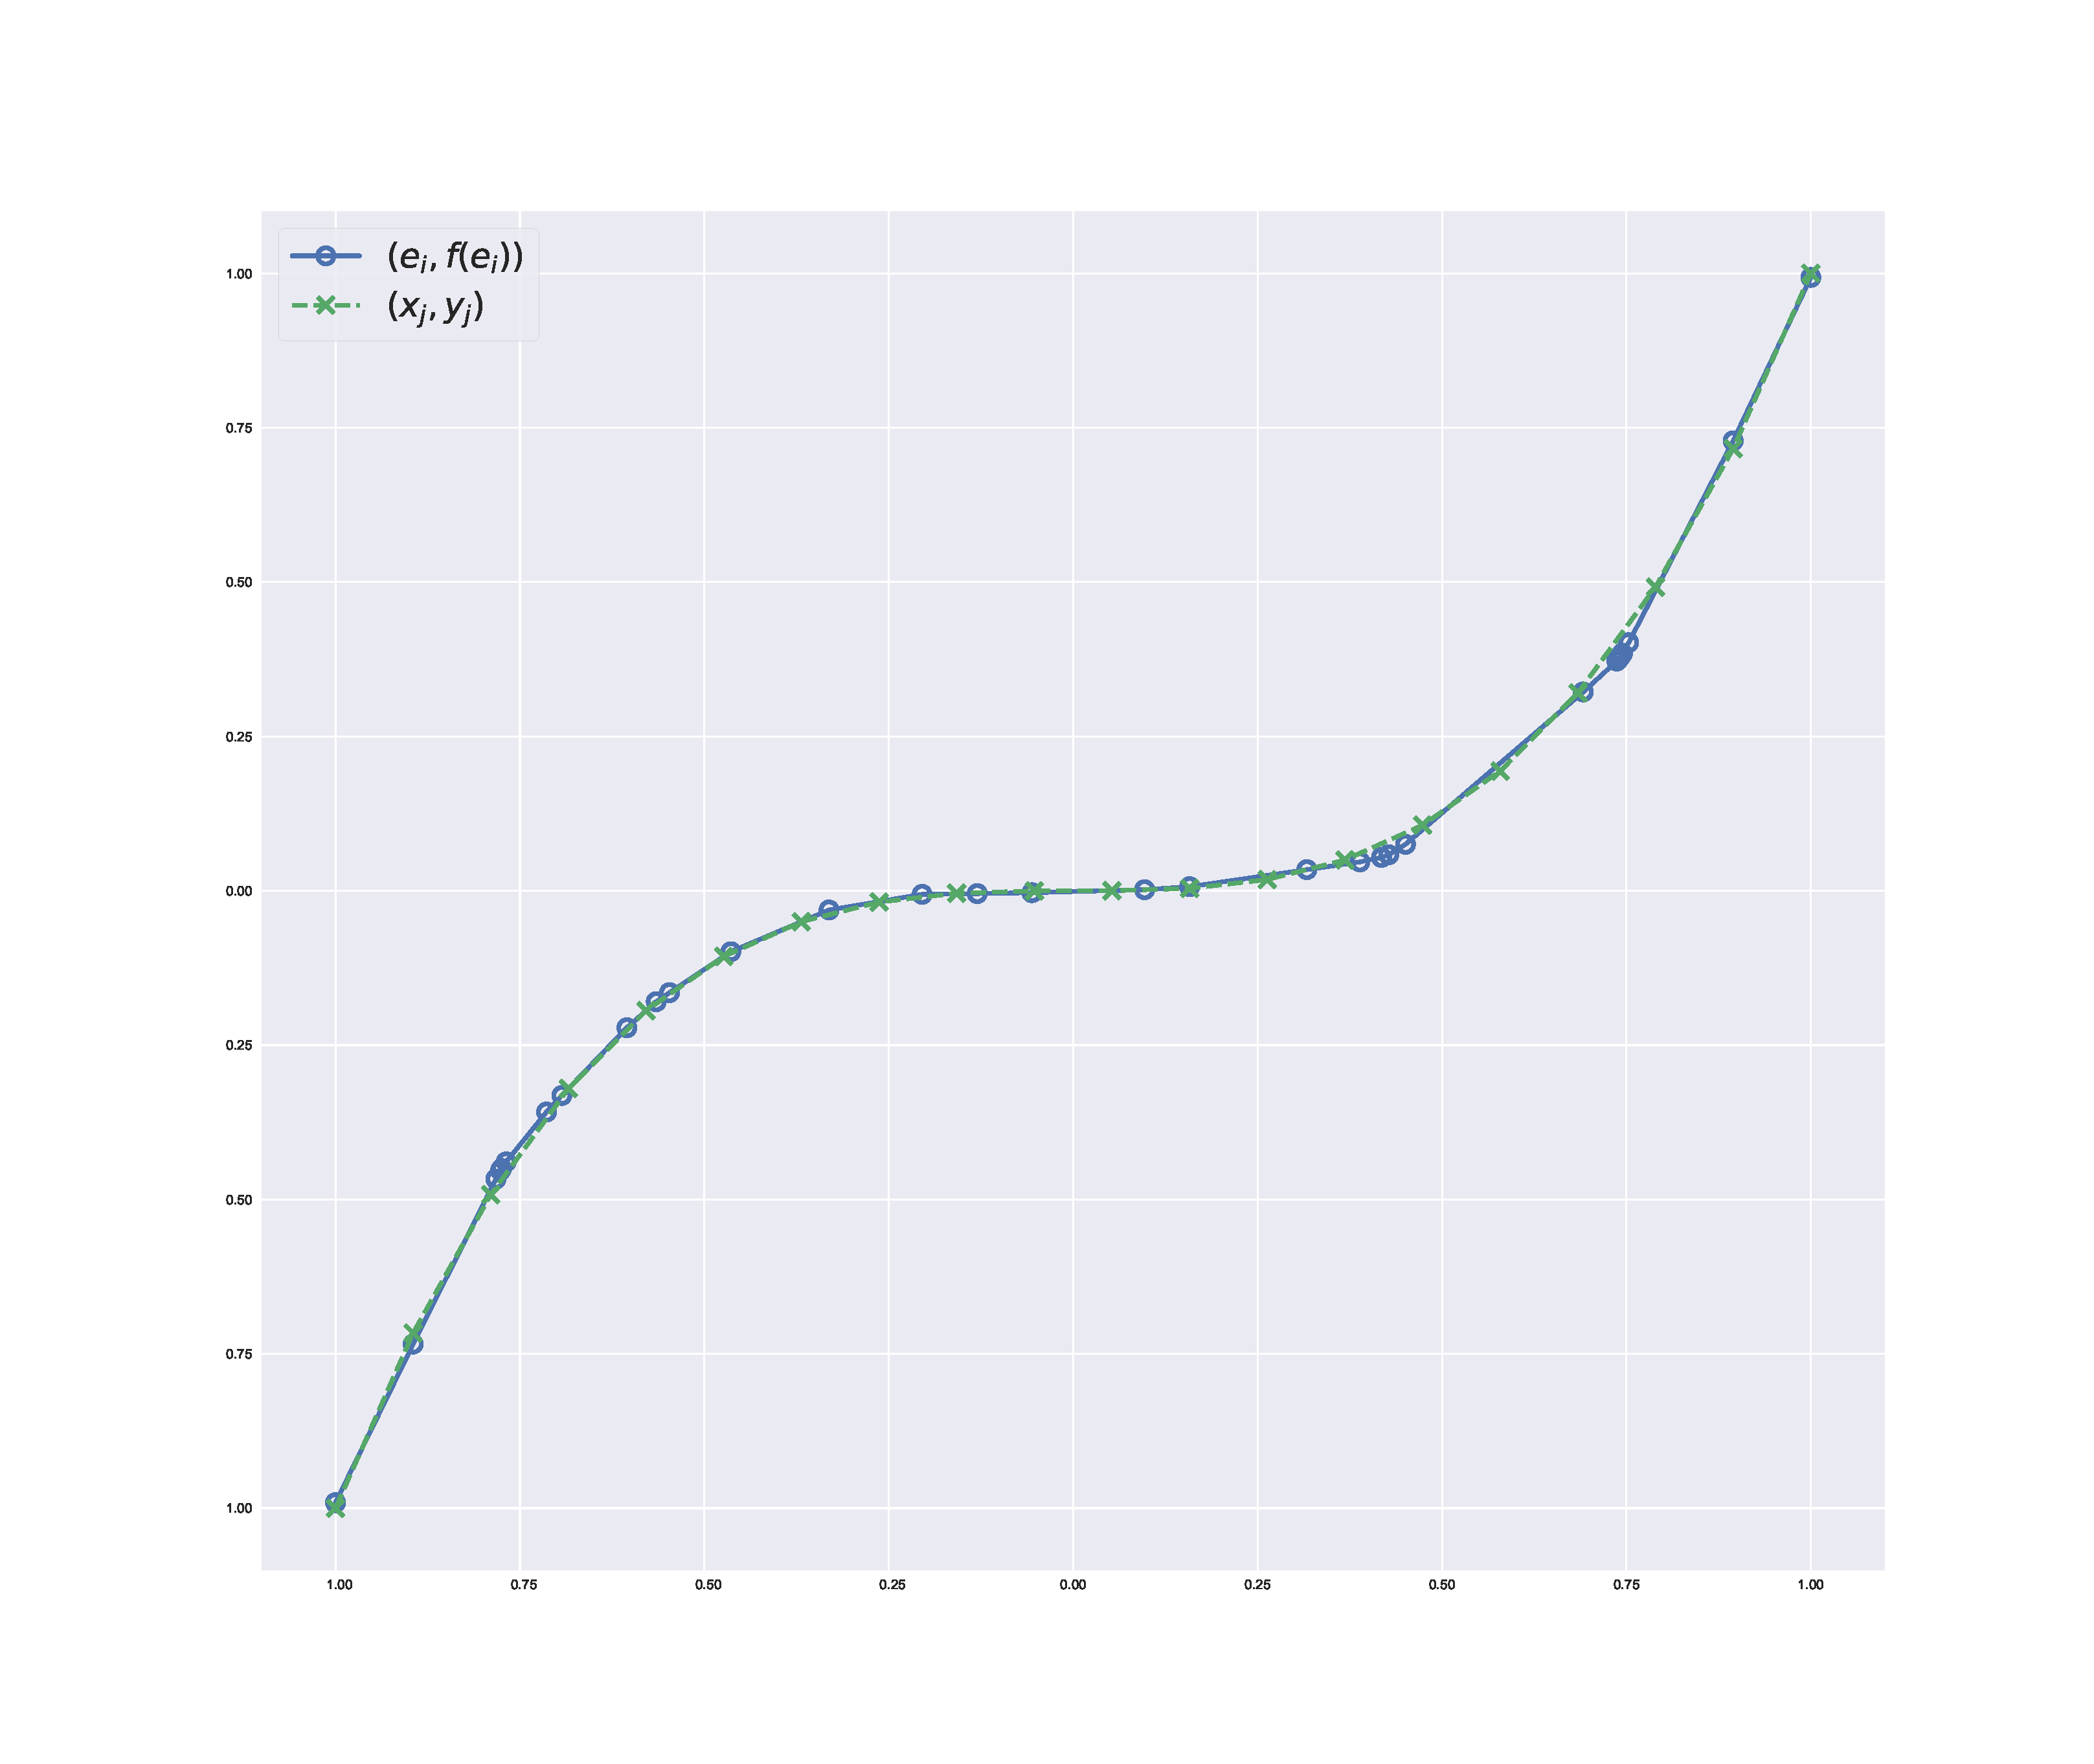
\includegraphics[width=\textwidth]{figures/knots2.pdf}
    \endminipage\hfill
    \minipage{0.5\textwidth}
    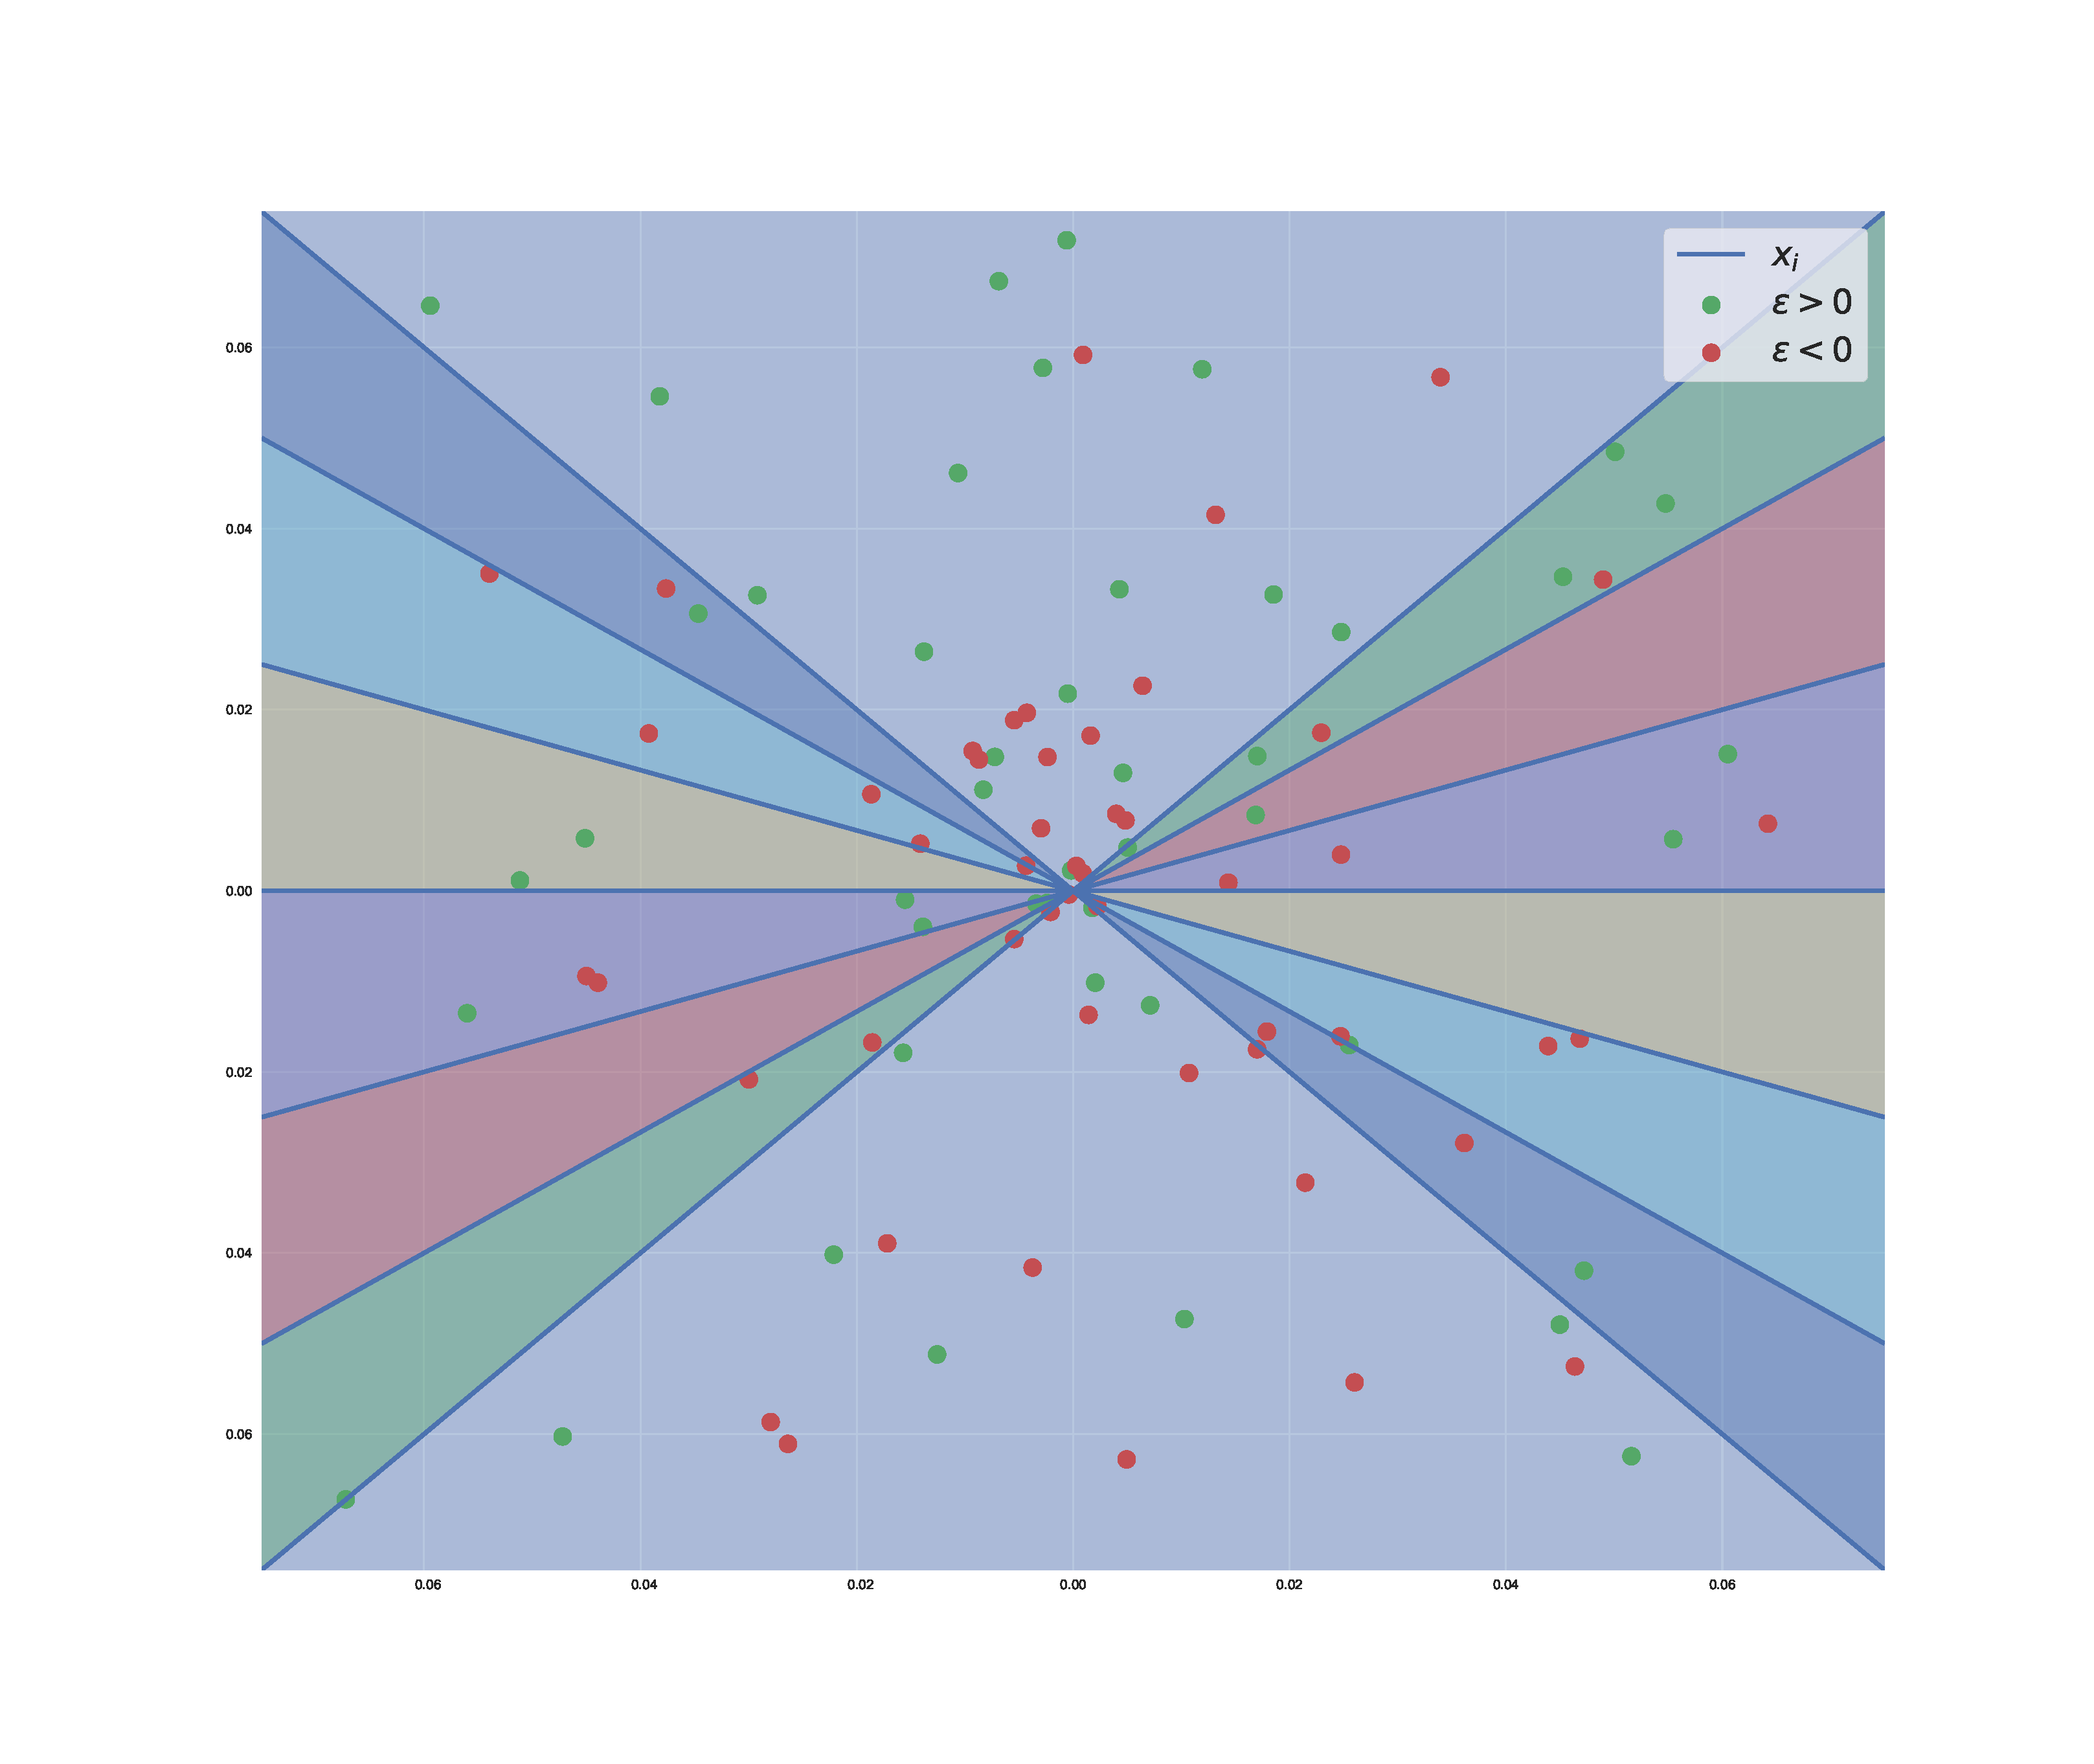
\includegraphics[width=\textwidth]{figures/phaseplot_eg.pdf}
    \endminipage\hfill
    
    
    \caption{\textit{Left:} input samples $(x, y) = (x_j, y_j)_{j=1}^s$ (blue x's) to which we fit a neural network $f_{\bm \xi}(x)$ using the least squares loss \eqref{eq:leastsquares}. $f_{\bm \xi}(x)$ is piecewise linear with the boundaries between pieces occurring at $(e_i, f_{\bm \xi}(e_i))_{i=1}^m$ (green circles). These points correspond to when the operand to one of the ReLUs in \eqref{eq:leastsquares} goes from positive to negative or vice-versa. \textit{Right:} the neurons $\xi_i = (\epsilon_i, u_i, v_i)$ plotted in $u-v$ space. The color of each neuron indicates the sign of $\epsilon_i$. Oberser that the samples $x_j$ correspond to the lines $u x_j + v = 0$ in this space. These sample lines divide the space into the colored regions which correspond to different activation patterns.}
    \label{fig:knots}
\end{figure}


\subsection{Gradient flow}

Our goal is to solve \eqref{eq:leastsquares} using the \emph{gradient flow} (the continuous-time limit of gradient descent) of the least squares loss:

\begin{equation}\label{eq:gradient_flow}
    \bm \xi(0) = \bm \xi_0, \qquad \bm \xi'(t) \in \partial L(\bm \xi(t)).
\end{equation}

Here $\partial L(\bm \xi)$ denotes the \emph{Clarke subdifferential}~\cite{clarke1975generalized}, since $L(\bm \xi)$ is only piecewise smooth. At generic smooth points $\bm \xi$, the subdifferential coincides with the gradient $\partial L(\bm \xi(t)) = \{\nabla L(\bm \xi)\}$. However, we argue in \todo{Section~\ref{todo}} that the discontinuities of the gradient play an important role in the dynamics in practice. For this reason, we subdivide the parameter space into \emph{regions} associated with different \emph{activation patterns} (Figure \ref{fig:knots})

\begin{equation}
    R(\bm \tau, \phi) = \{ (\epsilon, u, v) \, | \, \mathds 1 [u_j x_i + v_j \geq 0] = \tau_{ij}, \, \epsilon = \phi \}
\end{equation}
% \begin{equation}
%     R(\bm \tau,) = \{\bm \xi = (\bm \epsilon, \bm u, \bm v) \in \{-1, 0, 1\} \times \RR^{2m} \, | \, \mathds 1 \rangle (x_i, 1), (u_j, v_j) \rangle  = \tau_{ij},\, {\rm sign}(c_j) = \epsilon_j\}, \quad \bm \tau \in \{0,1\}^{s \times m}, \bm \epsilon \in \{-1,1\}^{m}.
% \end{equation}

If $R(\bm \tau, \phi)$ is not empty, it is a polyhedral cone containing the origin, and it is a product of ``sectors'' corresponding to the activation pattern of each neuron. It is important to note that, in our one-dimensional setting, every neuron can have \emph{at most} $2s$ activation patterns (out of the possible $2^s$ combinatorial types), which means that, for $R(\bm \tau, \phi)$ to be non-empty, the columns of $\bm \tau$ must be chosen among $2s$ possible vectors.
In the interior of a non-empty region $R(\bm \tau, \phi)$, the gradient of $L(\bm \xi)$ can be written as
\begin{equation}\label{eq:derivative_equations}
\begin{gathered}
\nabla L(\bm \xi)_i = \begin{bmatrix}\partial_{u_i} \\ \partial_{v_i}\end{bmatrix} = \epsilon_i \sum_{j=1}^s \tau_{ij} r_j \begin{bmatrix} x_j \\ 1\end{bmatrix}\\
\end{gathered}
\end{equation}
where $r_j = f_{\bm \theta}(x_j) - y_j$ is the $j$-th \emph{residual}. We note that the gradient $\nabla L(\bm \xi)$ is piecewise constant (see Figure~\ref{fig:reduced_grad}) with the discontinuities occurring at the boundaries between regions $R(\bm \tau, \phi)$. The signs $\bm \epsilon$ evolve during the gradient flow as follows:

\begin{equation}
    \epsilon(t) = \text{sign}(
\end{equation}

Finally, we remark that a solution $\bm \xi(t)$ to~\eqref{eq:gradient_flow} will in general converge to a first-order stationary point $\bm \theta^*$ where $0 \in \partial L(\bm \theta^*)$. For certain asymptotic (highly over-parameterized) regimes, it is possible to show convergence to global optima~\cite{du2018gradient,chizat2018global}. In our concrete low dimensional setting, we can state the following result.

\begin{proposition} Let $\bm \xi^* = (\bm \epsilon^*, \bm u^*, \bm v^*)$ be a critical point for $L(\bm \xi)$, and consider the matrix
\begin{equation}
    \bm M_{\bm u^* \bm v^*} = \big [ \langle (x_i, 1), (u_j^*, v_j^*) \rangle_+ \big ]_{ij} \in \RR^{s \times m}.
\end{equation}
If $\bm M_{\bm a^* \bm b^*}$ has full rank, then $L(\bm \theta^*) = 0$, so $\bm \theta^*$ is a global minimum. If $s< m$ and $e_1 \le \ldots \le e_m$ are the knots~\eqref{eq:knots} associated with $\bm \theta^*$, then a sufficient condition for $\bm M_{\bm a^* \bm b^*}$ to have full rank is that each interval $[-\infty, e_1],[e_1,e_2],\ldots,[e_m,\infty]$ contains at most one sample point $x_i$.
\end{proposition}





\subsection{Visualization of reduced parameters}


In the next section, we will illustrate our results by visualizing neurons as in Figure~\ref{fig:phaseplot_eg}. Here, every colored ``particle'' represents a single neuron of $f_{\bm \theta}$ using \emph{reduced coordinates} $\bm \xi$:
\begin{equation}\label{eq:reduced_params}
\bm \xi_i = (u_i,v_i) = (|c_i|a_i,|c_i| b_i), \qquad i=1,\ldots,m.
\end{equation}
The color of the particle indicates the sign $\epsilon_i \in \{+1,-1\}$ of $c_i$ (assuming it is non-zero). Each data point $x_i$ corresponds to a \emph{line} through the origin, namely $u x_i + v =0$. The $2s$ colored sectors indicate regions where neurons have a fixed activation patterns.

Note that although the reduced coordinates $(u_i,v_i)$ do not uniquely identify the parameters $(a_i,b_i,c_i)$, together with $\epsilon_i$ they determine the neuron as a \emph{function}, since $c_i[a_i x + b_i]_+ = \epsilon_i[u_i x + v_i]_+$.
Thus, the reduced parameters determine $f_{\bm \theta}$, but have $m$ fewer degrees of freedom (one per neuron) compared to $\bm \theta$. These degrees of freedom are indeed unnecessary because the association $\bm \theta \rightarrow f_{\bm \theta}$ is not injective. 

% On the other hand, we will argue in the next section that the knowledge of the initial parameters $\bm \theta(0)$ is sufficient recover  to ``lift'' a reduced representation and recover the true neurons.



\section{Training Dynamics}

In this section, we study the trajectories $\bm z(t)$ that are solutions of the two gradient flow equations \eqref{eq:kernel_gf} and \eqref{eq:adaptive_gf} corresponding to the kernel and adaptive regimes. 
%We analyze these in case where the number of neurons is infinite ($m = \infty$)


\subsection{Kernel Learning}

\note{This section needs more work} 
\note{We should point out that minimizing $\|c\|$ minimizes curvature for the uniform initialization, because this is a generally useful fact}

We first consider the dynamics of kernel learning in the limit when the number of neurons is infinite ($m = \infty$). In this regime, we only train the outer layer paramters $\bm c$. In phase space, this corresponds to neuron trajectories that move radially away from the origin (see Figure \ref{fig:trajectories}). In this setting, it is convenient to reparameterize our model as

\begin{equation}\label{eq:infinite_model}
    f_{\bm \theta}(x) = \int c_+(s) a_+(s)[x-s]_+ ds \, + \,  \int c_-(s) a_-(s)[s-x]_+ ds
\end{equation}

where $a_+, a_-, c_+, c_-$ are scalar functions corresponding to the distributions of positive and negative neurons \note{Joan, how should we argue that this is a valid way to go to the limit? It should be because we can integrate over scalings of $a, b$ without chaning loss or dynamics}
Use the scaling $1/\sqrt{m}$ and refer to prior work (NTK and Chizat, Bach), no need to redo the argument here. 

We introduce the following kernel
\begin{equation}
\begin{gathered}
    f(x) = \sum_{j=1}^s \alpha_j K(x_j, x) \text{ where } \\
    K(x, x') = \int a_+(s)^2[x - s]_+ [x' - s]_+ ds + \int a_-(s)^2[s - x]_+ [s - x']_+ ds\\
    = \int_{-\infty}^{\min x, x'} a_+(s)^2 (x - s)(x' - s) ds + \int_{\max x, x'}^\infty a_-(s)^2(s - x) (s - x')_+ ds.
\end{gathered}
\end{equation}

In the overparameterized case, we wish to solve least squares problem

\begin{equation}\label{eq:least_squares_op}
    \text{minimize } \|\bm c\|^2 \text{ s.t. } f_{\bm \theta}(\bm x) = \bm y.
\end{equation}

Solutions $f(x)$ can be written in terms of the kernel as

\begin{equation}~\label{eq:kernel_solution}
    \hat f(x) = \sum_{j=1}^s \alpha_j K(x_j,x),
\end{equation}

where $\alpha_j = K^{-1}(\bm y)$ and $K(x_i, x_j) = (\bm K_{c})_{ij}$. We note that the gradient flow will actually converge to this solution only if $\bm c(0)$ is initialized sufficiently close to the origin. Contrary to to the usual kernels considered in ReLU networks~\cite{cho2009kernel,bach2017breaking}, which consider neurons uniformly distributed over a sphere, it is natural in our setting to consider \emph{unform distributions} of neurons $a_+(s) = \mathds 1[k_0,k_1]$ (neurons with $a=1$ uniformly distributed in $[k_0, k_1]$) or $a_+(x) = a_-(s) = \mathds 1[k_0,k_1]$ (neurons with $a=1$ and $a=-1$ uniformly distributed in $[k_0, k_1]$). Interestingly, we note that these distributions of neurons lead to \emph{cubic spline interpolation}.

\begin{proposition} If $a_+(s) = \mathds 1[k_0,k_1]$ or $a_+(x) = a_-(s) = \mathds 1[k_0,k_1]$, the kernel $K(x,x')$ is a piecewise cubic polynomial in $x$ and $x'$. In particular, in the overparameterized setting, the solution~\eqref{eq:kernel_solution} will be an interpolating \emph{cublic spline}.
\end{proposition}

Another way to justify this result is to notice that if $f_{\bm \theta}$ is as in~\eqref{eq:infinite_model} with $a_+(x)$, then $f_{\bm \theta}''(x) = c_+(s)$. Hence, the interpolation is minimizing \emph{curvature}.
We remark that machine learning packages such as PyTorch use a uniform distribution for linear layer parameter initialization by default.
We verify that indeed, solutions to \eqref{eq:leastsquares} converge to cubic splines as $m$ grows in Figure~\ref{fig:cubic_splines}. We also point out that in Kernel Learning, early termination of gradient flow acts as a regularizer favoring smooth, non-interpolatory solutions (see \cite{NTKJacot} and Section~\ref{sec:implicit_regularizer}).



\subsection{Active Learning}

We now consider the dynamics of adaptive learning. In this regime, we train all network parameters, and reparameterize the model as 

%we only train the inner layer parameters $\bm a, \bm b$. In phase, space this corresponds to neuron trajectories which move along a piecewise constant gradient field  with boundaries corresponding to the boundaries of the activation regions, $R$ \eqref{eq:activatioon_region}.
%In this regime, it is convenient to 

\begin{equation}
    f_\mathbf{z}(x) = \frac{1}{m}\sum_{i=1}^m c_i \langle \tilde{x}, \theta_i \rangle_+~,
\end{equation}
with parameters $\mathbf{z}=(z_1\dots z_m)$, $z_i=(c_i ,\theta_i) \in \mathbb{R} \times S^1$, and  
where $\tilde{x} = (x, 1)$. %\bm v(\theta) \in S^1 = (\cos(\theta), \sin(\theta))$, and $\langle \cdot, \cdot \rangle_+$ is a ReLU. 
Thanks to the homogeneity of the ReLU activation function, this parametrisation represents the same functional space as the model using the standard parameterization (\ref{eq:standard_parameterization}).
We use the scaling in $1/m$ in order to obtain an asymptotic behavior as $m\to \infty$ whereby both first and second layer weights 
move away from their initialization under gradient descent and the kernel dynamics no longer apply-- the \emph{active learning} regime of \cite{chizat2018note}. 

Using this normalization, and following the mean-field formulation of single-hidden layer neural networks of \cite{meimontanari, chizat2018global, rotskoffeve}, we express the function as an expectation with respect to a probability measure $\mu$ over the cylinder $\mathcal{D} = \mathbb{R} \times S^1$:
\begin{equation}
    f_\mathbf{z}(x) = \int_\mathcal{D} \varphi(z;x) \mu^{(m)}(dz)~,
\end{equation}
where $\varphi(z;x):=c \langle \tilde{x}, \theta_i \rangle_+$ and $\mu^{(m)}(z) = \frac{1}{m} \sum_{i=1}^m \delta_{z_i}(z)$ 
is the empirical measure determined by the $m$ particles $z_i$, $i=1\dots m$.
The least squares loss in this case becomes 
\begin{eqnarray}
    L(\mathbf{z}) &=& \frac{1}{2}\| f_\mathbf{z} - y \|_\mathcal{X}^2 \\
    &=& \frac{1}{2}\| y\|^2_\mathcal{X} - \langle f_\mathbf{z} , y \rangle_\mathcal{X} + \frac{1}{2}\| f_\mathbf{z} \|^2_\mathcal{X} \\
    &=& C_y - \frac{1}{m} \sum_{i=1}^m \langle \varphi_{z_i} , y \rangle_\mathcal{X} + \frac{1}{2m^2} \sum_{i,i'=1}^m \langle \varphi_{z_i} ,\varphi_{z_{i'}} \rangle_\mathcal{X} ~,
\end{eqnarray}
where $\langle f, g \rangle_\mathcal{X} := \sum_{j=1}^s f(x_j) g(x_j)$ is the empirical dot-product. 
This loss may be interpreted as the Hamiltonian of a system of $m$-interacting particles, under external 
field $F$ and interation kernel $K$ defined respectively by 
\begin{equation}
F(z):= \langle \varphi_z, y \rangle_\mathcal{X} ~,~K(z, z'):= \langle \varphi_{z} ,\varphi_{z'} \rangle_\mathcal{X}~.    
\end{equation}
We may also express this Hamiltonian in terms of the empirical measure, by abusing notation
$$L(\mu^{(m)}) = C_y - \int_\mathcal{D} F(z) \mu^{(m)}(dz) + \frac{1}{2} \iint_{\mathcal{D}^2} K(z,z') \mu^{(m)}(dz) \mu^{(m)}(dz')~.$$

A direct calculation shows that the gradient $\nabla_{z_i} L(\mathbf{z})$ can be written as 
$$\frac{m}{2} \nabla_{z_i} L(\mathbf{z}) = \nabla_z V(z_i; \mu^{(m)})~,$$%\text{ with } $$
where $V$ is the potential function 
\begin{equation}
\label{eq:potential}
    V(z;\mu):= -F(z) + \int_\mathcal{D} K(z, z') \mu(dz')~.
\end{equation}
The gradient flow in the space of parameters $\mathbf{z}$ can be now interpreted in terms of a gradient flow in the space of measures over $\mathcal{D}$ by using the notion of Wasserstein gradient flows \cite{meimontanari, chizat2018global, rotskoffeve}. Indeed, 
equation \ref{eq:potential} shows that particles evolve in $\mathcal{D}$ by ``feeling" a velocity field $\nabla V$ defined in $\mathcal{D}$. 
This formalism allows us now to describe the dynamics independently of the number of neurons $m$, by replacing the empirical measure $\mu^m$ 
by any generic probability measure $\mu$ in $\mathcal{D}$. The evolution of a measure under a generic time-varying vector field is given by the 
so-called continuity equation:
\begin{equation}
\label{eq:continuity}
    \partial_t \mu_t = \mathrm{div} ( \nabla V \mu_t)~,
\end{equation}
understood in the weak sense, ie 
$\partial_t \left(\int_\mathcal{D} \phi(z) \mu_t(dz)\right) = - \int \langle \nabla \phi(z), \nabla V(z;\mu_t) \rangle \mu_t(dz)$, 
$\forall \phi \in C^1_c(\mathcal{D})$ continuously differentiable and with compact support. The global 
convergence of this PDE for interaction kernels arising from single-hidden layer neural networks has been 
 established under mild assumptions in \cite{meimontanari, chizat2018global, rotskoffjoan}. Although 
 the conditions for global convergence hold in the mean field limit $m \to \infty$, a propagation-of-chaos 
 argument from statistical mechanics gives Central Limit Theorems for the behavior of finite-particle systems 
 as fluctuations of order $1/\sqrt{m}$ around the mean-field solution; see \cite{rotskoffeve, rotskoffjoan} for further details. 

The dynamics in $\mathcal{D}$ are thus described by the velocity field $\nabla V(z; \mu_t)$, which depends on the current 
state of the system through the measure $\mu_t(z)$, describing the probability of encountering a particle
at position $z$ at time $t$. We emphasize that equation (\ref{eq:continuity}) is valid 
for any measure, including the empirical measure $\mu^{(m)}$, and is therefore an exact model for 
the dynamics in both the finite-particle and infinite-particle
regime. Let us now describe its specific form in the case of the empirical loss given above. 

Assume without loss of generality that the datapoints $x_j \in \mathbb{R}$, $j\leq s$ satisfy $x_j \leq x_{j'}$ whenever $j < j'$.
Denote 
$$\mathcal{C}_j := \{ j' ; j' \leq j\} \text{ for } j=1\dots s,~\mathcal{C}_{s+j} := \{ j' ; j' > j \},\text{ for }j=1\dots s-1~.$$
We verify that for each $j$, the angles $\alpha_j = \arctan(x_j) \pm \pi/2$ partition the circle $S^1$ into $2s-1$ regions $\mathcal{A}_k$, 
which are in one-to-one correspondence with the sets $\mathcal{C}_k$, in the sense that 
$$\theta \in \mathcal{A}_k \Longleftrightarrow \{j ; \langle \tilde{x}_j , \theta \rangle \geq 0 \} = \mathcal{C}_k~.$$
\note{(These are the same as $R(\bm \tau)$ defined above, let's make the notation consistent)}
We also denote by $\mathcal{B}_j$ 
%$\mathcal{B}_j = \{ \theta; \theta \in (\alpha_j - \pi/2, \alpha_j+\pi/2)\}$ for $j=1\dots s$
the half-circle where $\langle \tilde{x}_j, \theta\rangle \geq 0$. Let $t(\theta)$ be the tangent vector of $S^1$ at $\theta$.

Let $z=(c,\theta)$, and suppose $\theta \in \mathcal{A}_k$. From (\ref{eq:potential}), the angular velocity field $\nabla_\theta V(z; \mu_t)$ is given by 
\begin{eqnarray}
\label{eq:meanfield1}
    \nabla_\theta V(z; \mu_t) &=& -\nabla_\theta F(z) + \int_\mathcal{D} \nabla_\theta K(z, z') \mu_t(dz') \nonumber \\
    &=& -c\left( \sum_{j \in \mathcal{C}_k} y_j \langle \tilde{x}_j, t(\theta)\rangle  -\int_\mathcal{D} c'\sum_{j \in \mathcal{C}_k} \langle \tilde{x}_j,t(\theta)\rangle \langle \tilde{x}_j, \theta' \rangle_+ \mu_t(dc', d\theta') \right) \nonumber \\
    &=& -c \sum_{j \in \mathcal{C}_k} \langle \tilde{x}_j, t(\theta)\rangle \left(y_j - \int_{\mathbb{R} \times \mathcal{B}_j} c' \langle \tilde{x}_j, \theta' \rangle \mu_t(dc', d\theta') \right) \nonumber \\
    &=& c \left \langle \sum_{j \in \mathcal{C}_k} r_j(t) \tilde{x}_j, t(\theta) \right \rangle~,
\end{eqnarray}
where 
$$r_j(t) = f_{\mu_t}(x_j) - y_j =    \int_{\mathbb{R} \times \mathcal{B}_j} c \langle \tilde{x}_j,\theta  \rangle \mu_t(dc, d\theta)  - y_j$$
is the residual at point $x_j$ at time $t$. 
Similarly, the field in the direction of the charges is given by
\begin{equation}
\label{eq:meanfield2}
    \nabla_c V(z; \mu_t) =  \left \langle \sum_{j \in \mathcal{C}_k} r_j(t) \tilde{x}_j, \theta \right \rangle ~.
\end{equation}
Equations (\ref{eq:meanfield1}, \ref{eq:meanfield2}) show that the dynamics are entirely controlled by the 
$s$-dimensional vector of residuals $\mathbf{r}(t)=(r_1(t), \dots r_s(t))$, and that the flow is piece-wise linear 
on each cylindrical region $\mathbb{R} \times \mathcal{A}_k$. 
Under the assumptions that ensure 
global convergence of (\ref{eq:continuity}), we have $\lim_{t \to \infty} L(\mu(t)) = 0$, 
and therefore $\| \mathbf{r}(t) \| \to 0$. The oscillations of $\mathbf{r}(t)$ as it converges 
to zero determine the relative orientation of the flow within each region. 

Observe that for each $j$, 
\begin{eqnarray}
\label{eq:oderesiduals}
\dot{r}_j(t) &=& \partial_t f_{\mu_t}(x_j) = \partial_t \left( \int_\mathcal{D} \varphi(z;x_j) \mu_t(dz) \right) \nonumber \\ 
&=& - \int_\mathcal{D} \langle \nabla_z \varphi(z;x_j), \nabla V(z;\mu_t) \rangle \mu_t(dz) \nonumber \\
&=& - \int_\mathcal{D} \left(  \nabla_\theta \varphi(z;x_j) \cdot \nabla_\theta V(z;\mu_t)  +  \nabla_c \varphi(z;x_j) \cdot \nabla_c V(z;\mu_t)  \right) \mu_t(dz) \nonumber \\
&=& -\sum_{k; \mathcal{A}_k \subset \mathcal{B}_j} \int_{\mathbb{R} \times \mathcal{A}_k} \left( c^2  \tilde{x}_j^\top (t(\theta)t(\theta)^\top) (\sum_{j' \in \mathcal{C}_k} r_{j'}(t) \tilde{x}_{j'}) + \tilde{x}_j^\top (\theta \theta^\top) (\sum_{j' \in \mathcal{C}_k} r_{j'}(t) \tilde{x}_{j'}) \right) \mu_t(dz) \nonumber  \\
&=& -\tilde{x}_j^\top \sum_{k; \mathcal{A}_k \subset \mathcal{B}_j}  \Sigma_k(t) (\sum_{j' \in \mathcal{C}_k} r_{j'}(t) \tilde{x}_{j'})~, 
\end{eqnarray}
where 
$$\Sigma_k(t) = \int_{\mathbb{R} \times \mathcal{A}_k} \left(c^2 t(\theta)\, t(\theta)^\top + \theta\, \theta^\top\right) \mu_t(dc,d\theta) $$
tracks the covariance of the measure along each 
cylindrical region. Equation (\ref{eq:oderesiduals}) 
defines a system of ODEs for the residuals $\mathbf{r}(t)$, but its coefficients are time-varying, and behave roughly as quadratic terms in $\mathbf{r}(t)$ (since they are second-order moments of the measure whereas the residuals are first-order moments). It may be possible to obtain asymptotic control of the oscillations $\mathbf{r}(t)$ by applying Duhamel's principle, 

Although the analytical solution of the PDE and ODE above is out of the scope of this work, we can use the flow equations above to argue qualitatively that the dynamics are now fundamentally different than in the kernel regime, 
and in particular they become \emph{data-adaptive}. In the cylindrical parametrisation, the kernel dynamics 
only move the charges, thus the angular distribution $\bar{\mu}(\theta) = \int_\mathbb{R} \mu(dc, \theta)$ equals the initial distribution 
and does not adapt to the input data. 

Let $z=(c,\theta)$ with $\theta$ at a boundary of two regions $\mathcal{A}_k$, $\mathcal{A}_{k+1}$. The velocity field is modified at the transition  by 
$$
\nabla V(z)\lvert_{\mathcal{A}_k} - \nabla V(z)\lvert_{\mathcal{A}_{k+1}} = r_{j*}(t) \left( 
\begin{array}{c}
c  \langle \tilde{x}_{j*}, t(\theta) \rangle \\
\langle \tilde{x}_{j*}, \theta \rangle
\end{array}\right)
~,$$
where $j_*$ is such that $\langle \tilde{x}_{j*}, \theta \rangle =0$ since $\theta$ is at the boundary of $\mathcal{A}_k$. It follows that the only discontinuity is in the angular direction, of magnitude $|c\, r_{j*}(t)|$, since $|\langle \tilde{x}_{j*}, t(\theta) \rangle| =1$.

An interesting phenomena arises when the angular components of $\nabla V(z)\lvert_{\mathcal{A}_k}$ and $\nabla V(z)\lvert_{\mathcal{A}_{k+1}}$ have opposite signs, corresponding to an `attractor' (resp `repulsor') that attracts/repels particles along the direction given by $\tilde{x}_{j*}$. By denoting $\alpha_k = \left \langle \sum_{j \in \mathcal{C}_k} r_j(t) \tilde{x}_j, t(\theta) \right \rangle$, from (\ref{eq:meanfield1}) we deduce that this occurs when
\begin{equation}
 \left|  \alpha_k \right| < |r_{j*}(t)| \text{ and } \text{sign}(\alpha_k) \neq \text{sign}(r_{j*}(t))~.    
\end{equation}
In words, mass will concentrate towards input points where the residual is currently large and of opposite sign from a weighted average of neighboring residuals. This is in stark contrast with the kernel dynamics, where there is no adaptation to the input datapoints. 


%Let $\mathbf{M} $




% The gradient flow in this parameterization is

% \begin{equation}
%     \begin{bmatrix}
%         c_i'(t)\\
%         \theta_i'(t)
%     \end{bmatrix} = 
%     \begin{bmatrix}
%         \sum_{j=1}^s =  
%     \end{bmatrix}
% \end{equation}
% regime where\theta'(t) $\delta_i \ll \|  = \xi_i \|$. In this regime, neurons move parallel to the reduced gradient field $\nabla \tilde{L}(\bm \xi)$ (see Figure \ref{fig:trajectories}). These trajectories are equivalent to those when training only the bottom layer parameters $(\bm a, \bm b)$ while keeping the top layer ($\bm c$) fixed. To understand the dynamics in this regime, we write the function $f$ in terms of the reduced parameters

% \begin{equation}
%     f_{\bm \xi}(x) = \sum_{i=1}^m \langle (x, 1), (u_i, v_i) \rangle_+ 
% \end{equation}

% The gradient of the loss with respect to the reduced parameters is 
% \begin{equation}\label{eq:grad_reduced}
%     \nabla \tilde{L}(\bm \xi)_i = \sum_{i=1}^s (f_{\bm \xi}(x_j) - y_j) \epsilon_i \tau_{ij} \begin{bmatrix}x_j \\ 1\end{bmatrix} 
% \end{equation}



% which is a piecewise constant function with the boundary between pieces occuring along the sample lines $u x_j + v = 0, j = 1 \ldots s$ (see Figure~\ref{fig:reduced_grad}). While the gradient field is in general discontinuous on the boundary of a sample, the component along a sample line is continuous







\subsection{Mixed Learning: Interpolating Kernel and Adaptive Learning}

In practice, the dynamics of gradient flow are a combination of the Kernel and Adaptive regimes. We can understand how much each regime contributes to the dynamics by considering the following conserved quantity:

\begin{lemma} \label{le:fixed_delta}
If $\bm \theta(t) = (\bm a(t), \bm b(t), \bm c(t))$ is a solution of the gradient flow \eqref{eq:gradient_flow}, then the quantities
\begin{equation}\label{eq:invariants}
\bm \delta = (\delta_i = c_i(t)^2 - a_i(t)^2 - b_i(t)^2)_{i=1}^m
\end{equation}
remain constant for all $t$. In particular, given a phase representation of a neuron $(\epsilon_i, u_i,v_i) = (\text{sign}(c_i), |c_i|a_i,|c_i|b_i)$, we can uniquely recover the original neuron $(a_i,b_i,c_i)$ since
\begin{equation}\label{eq:c_uv}
    c_i^2 = \frac{\delta_i + \sqrt{\delta_i^2 + 4 (u_i^2 + v_i^2)}}{2}. 
\end{equation}
\end{lemma}

Lemma~\ref{le:fixed_delta} allows us to analyze the dynamics in phase space without loss of generality. We can thus write the function and loss in phase space

\begin{equation}
    \tilde{f}_{\bm \xi}(x) = \sum_{j=1}^m \epsilon_i [ u_i x + v_i]_+.
\end{equation}
\begin{equation}
    \tilde L(\bm \xi) = \sum_{i=1}^s |\tilde{f}_{\bm \xi}(x_i) - y_i|^2, \qquad \bm \xi = (\bm \epsilon, \bm u, \bm v),  
\end{equation}

and consider the evolution of the parameters $\bm u$ and $\bm v$ during gradient flow. Note that so long as the signs, $\epsilon_i$ stay fixed, the trajectories of $\bm u$ and $\bm v$ will allow us to understand the trajectories of $\bm a$, $\bm b$ and $\bm c$. In that sense, the analysis here is \emph{local} within a time window with fixed $\epsilon$.

\begin{theorem}\label{thm:reduced_parameter_grad}
Let $\bm \theta(t)$ be an integral curve for the gradient flow \eqref{eq:gradient_flow} of $L(\bm \theta)$, and let $\bm \delta = (\delta_i) \in \RR^m$ be the vector of invariants~\eqref{eq:invariants}, which depend only on the initialization $\bm \theta(0)$. If $\bm \xi(t) = (\bm \epsilon, \bm u(t), \bm v(t))$ is curve of reduced parameters corresponding to $\bm \theta(t)$, then we have that
\begin{equation}
\begin{bmatrix}
u_i'(t)\\
v_i'(t)
\end{bmatrix} =
\bm P_{\delta_i}(u_i,v_i)
\begin{bmatrix}
\nabla_{u_i} \tilde L (\bm \xi)\\
\nabla_{v_i} \tilde L (\bm \xi)\\
\end{bmatrix},
\quad i=1,\ldots,m,
\end{equation}
where
\begin{equation}\label{eq:neuron_kernel}
\bm P_\delta(u_i,v_i) = \begin{bmatrix}
    a_i^2 + c_i^2  & 
    a_i b_i        \\
    a_i b_i               & 
    b_i^2 + c_i^2\\
\end{bmatrix} = 
\begin{bmatrix}
\frac{u_i^2}{c(u_i, v_i)^2} + c(u_i, v_i)^2 & \frac{u_i v_i}{c(u_i, v_i)^2}\\
\frac{u_i v_i}{c(u_i, v_i)^2} &  \frac{v_i^2}{c(u_i, v_i)^2} + c(u_i, v_i)^2\\
\end{bmatrix},
\end{equation}

and $c(u_i, v_i)^2 = \frac{\delta_i + \sqrt{\delta_i^2 + 4 (u_i^2 + v_i^2)}}{2}$
\end{theorem}

It is easy to verify that the eigenvalue-eigenvector pairs of $\bm P_{\delta_i}(u_i,v_i)$ are
\begin{align}
    (\lambda_1, \bm w_1) &= (a_i^2+ b_i^2 + c_i^2, (u_i,v_i))
    \label{eq:radial_eigenval}\\
    (\lambda_2, \bm w_2) &= (c_i^2, (-v_i,u_i)) 
    \label{eq:tangential_eigenval}
\end{align}
which define two types of trajectories. We can understand the dynamics of a neuron as a mix between these two types. In fact, writing $\rho_i = u_i^2 + v_i^2$, it is straightforward to verify that:

\begin{itemize}
    \item If $\rho_i \ll |\delta_i|$ and $\delta < 0$, then the eigenvector $\bm w_1$ dominates and $\xi'(t) \propto \xi$ causing the neuron moves \emph{radially} in phase space.
    \item If $\rho_i \ll |\delta_i|$ and $\delta > 0$, then the eigenvector $\bm w_2$ dominates and $(\dot u_i(t), \dot v_i(t)) \propto \nabla_{u_i} \tilde L(\bm \xi(t))$, causing the neuron to parallel to the vector field $\nabla \tilde L(\bm \xi)$.
\end{itemize}

Figure~\ref{fig:trajectories} shows the trajectories corresponding to different values of $\delta_i$ for a neuron. The extreme cases of $\delta = -\infty$ and $\delta = +\infty$ correspond exactly to the Kernel and Adaptive regimes respectively. 


\begin{figure}\label{fig:trajectories}
    \centering
    \minipage{0.33\textwidth}
    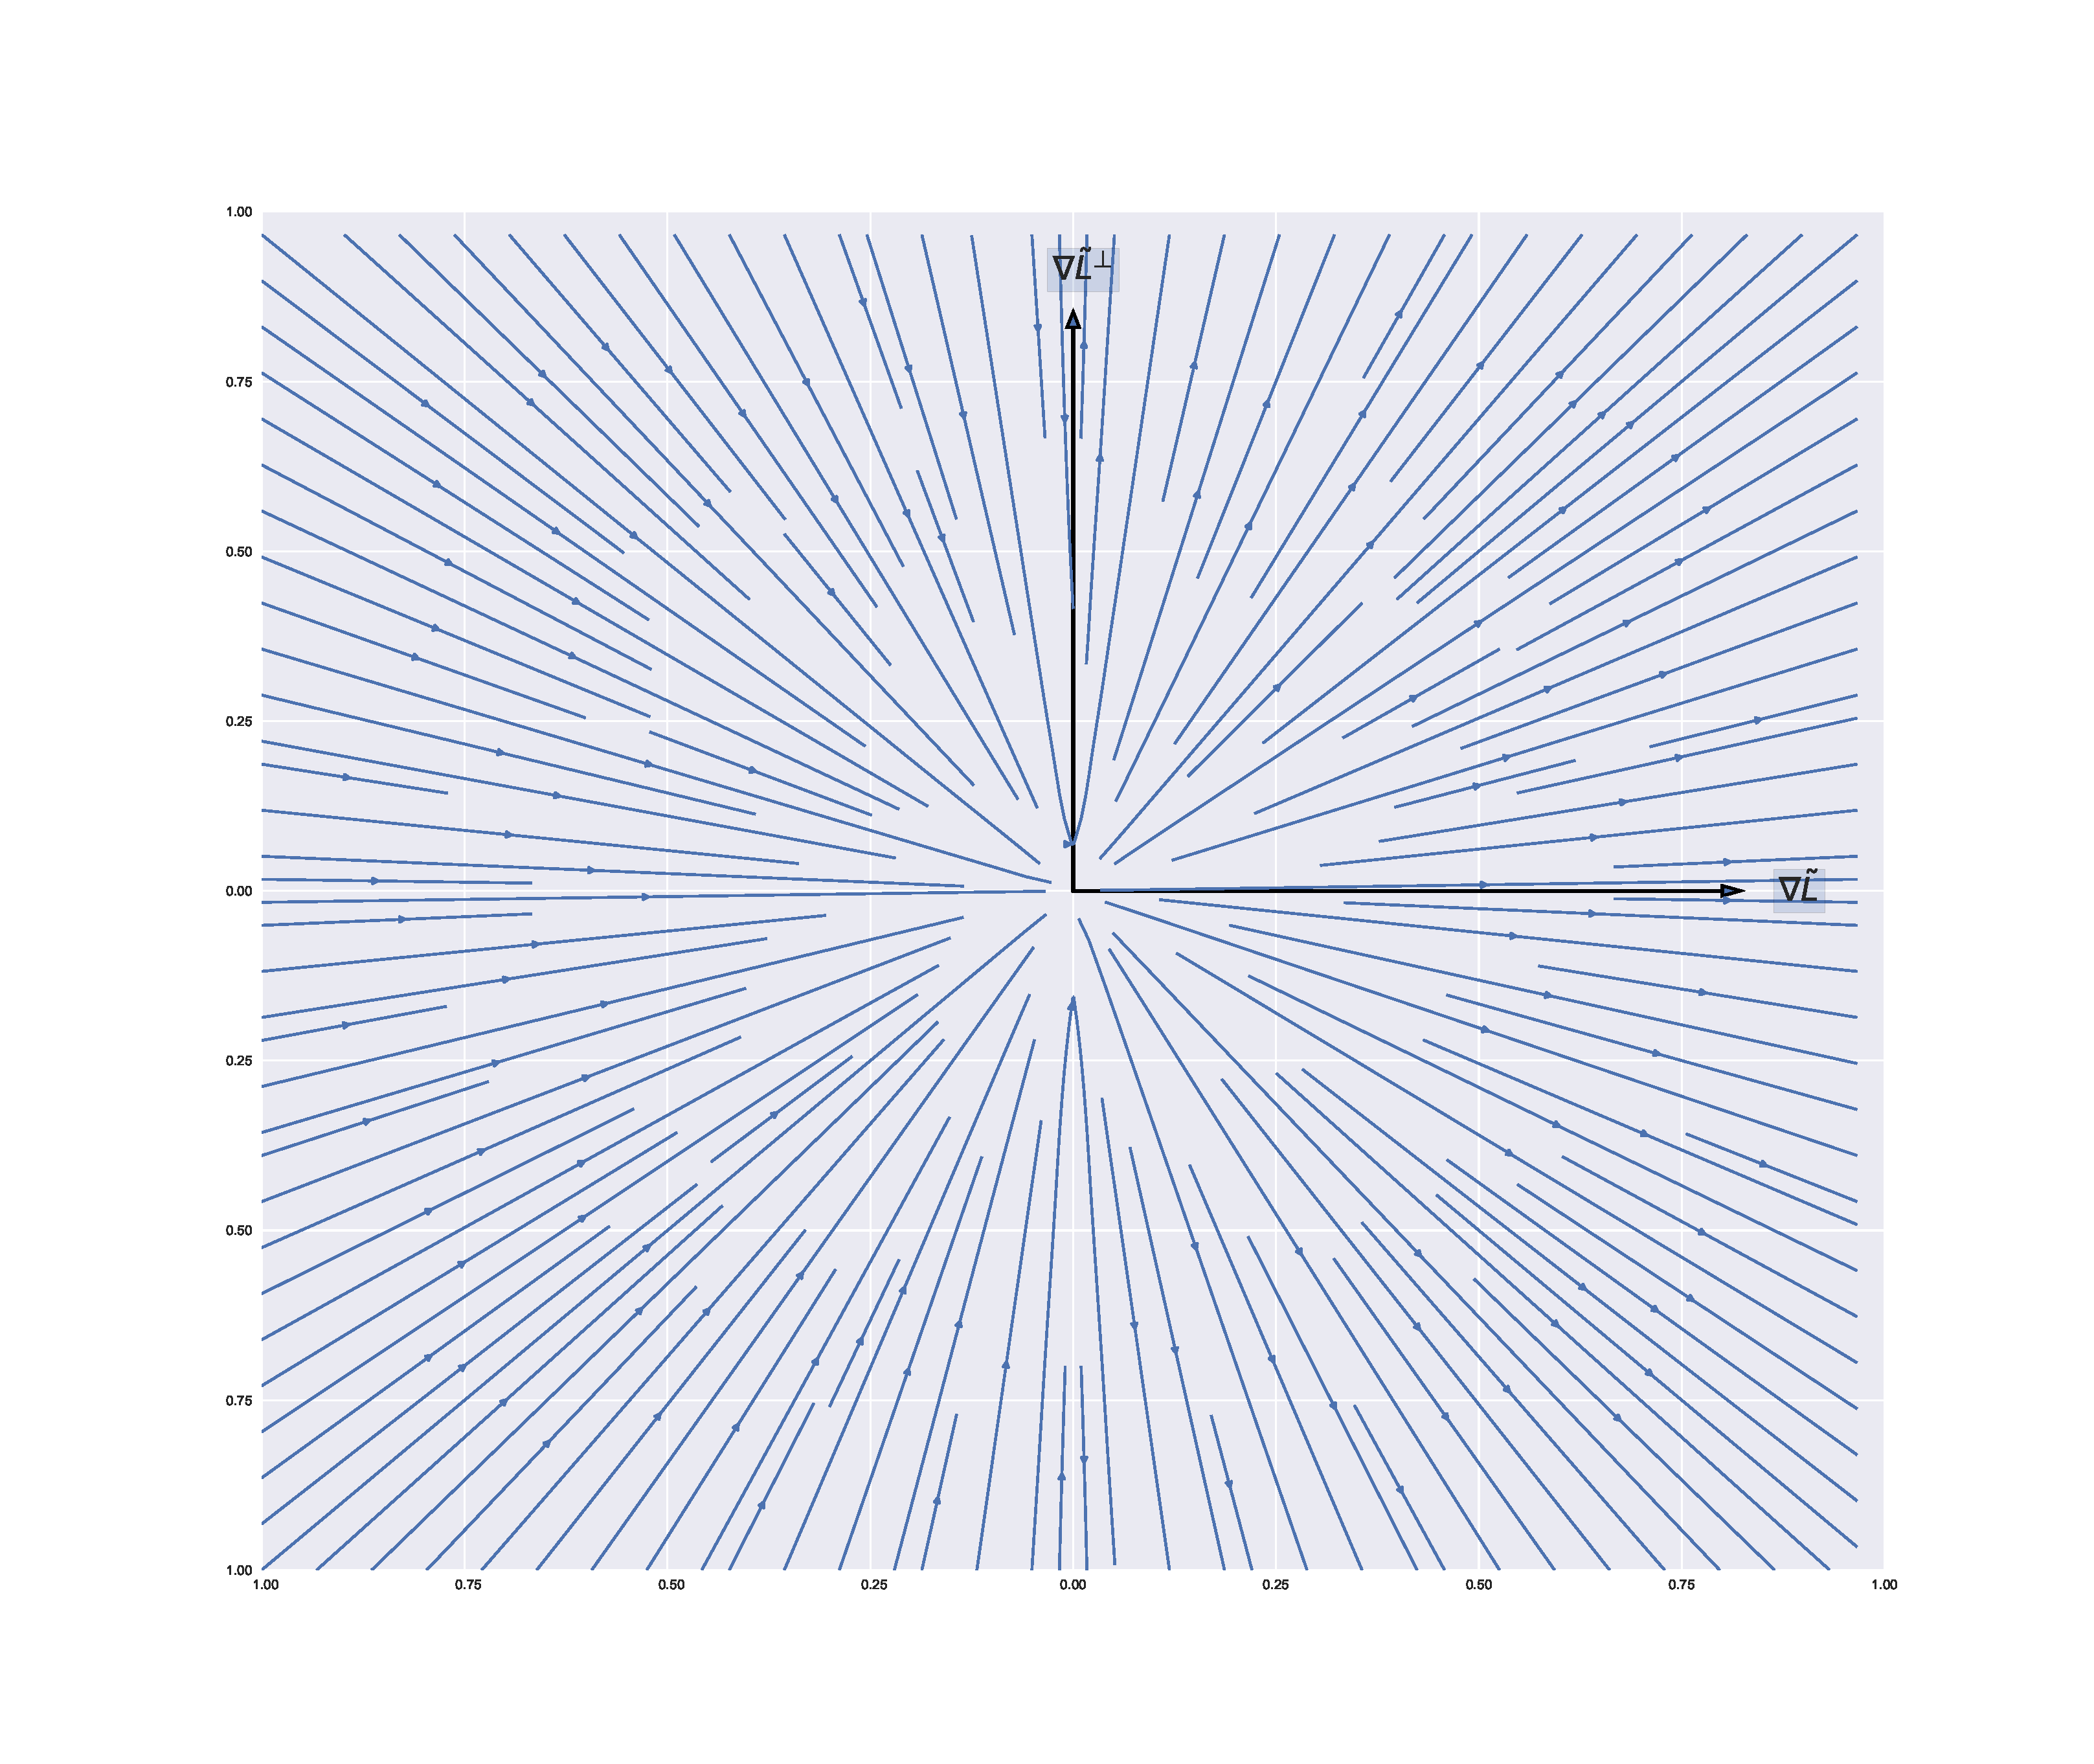
\includegraphics[width=\linewidth]{figures/dynamics_delta_-100.pdf}
    \endminipage\hfill
    % \minipage{0.2\textwidth}
    % 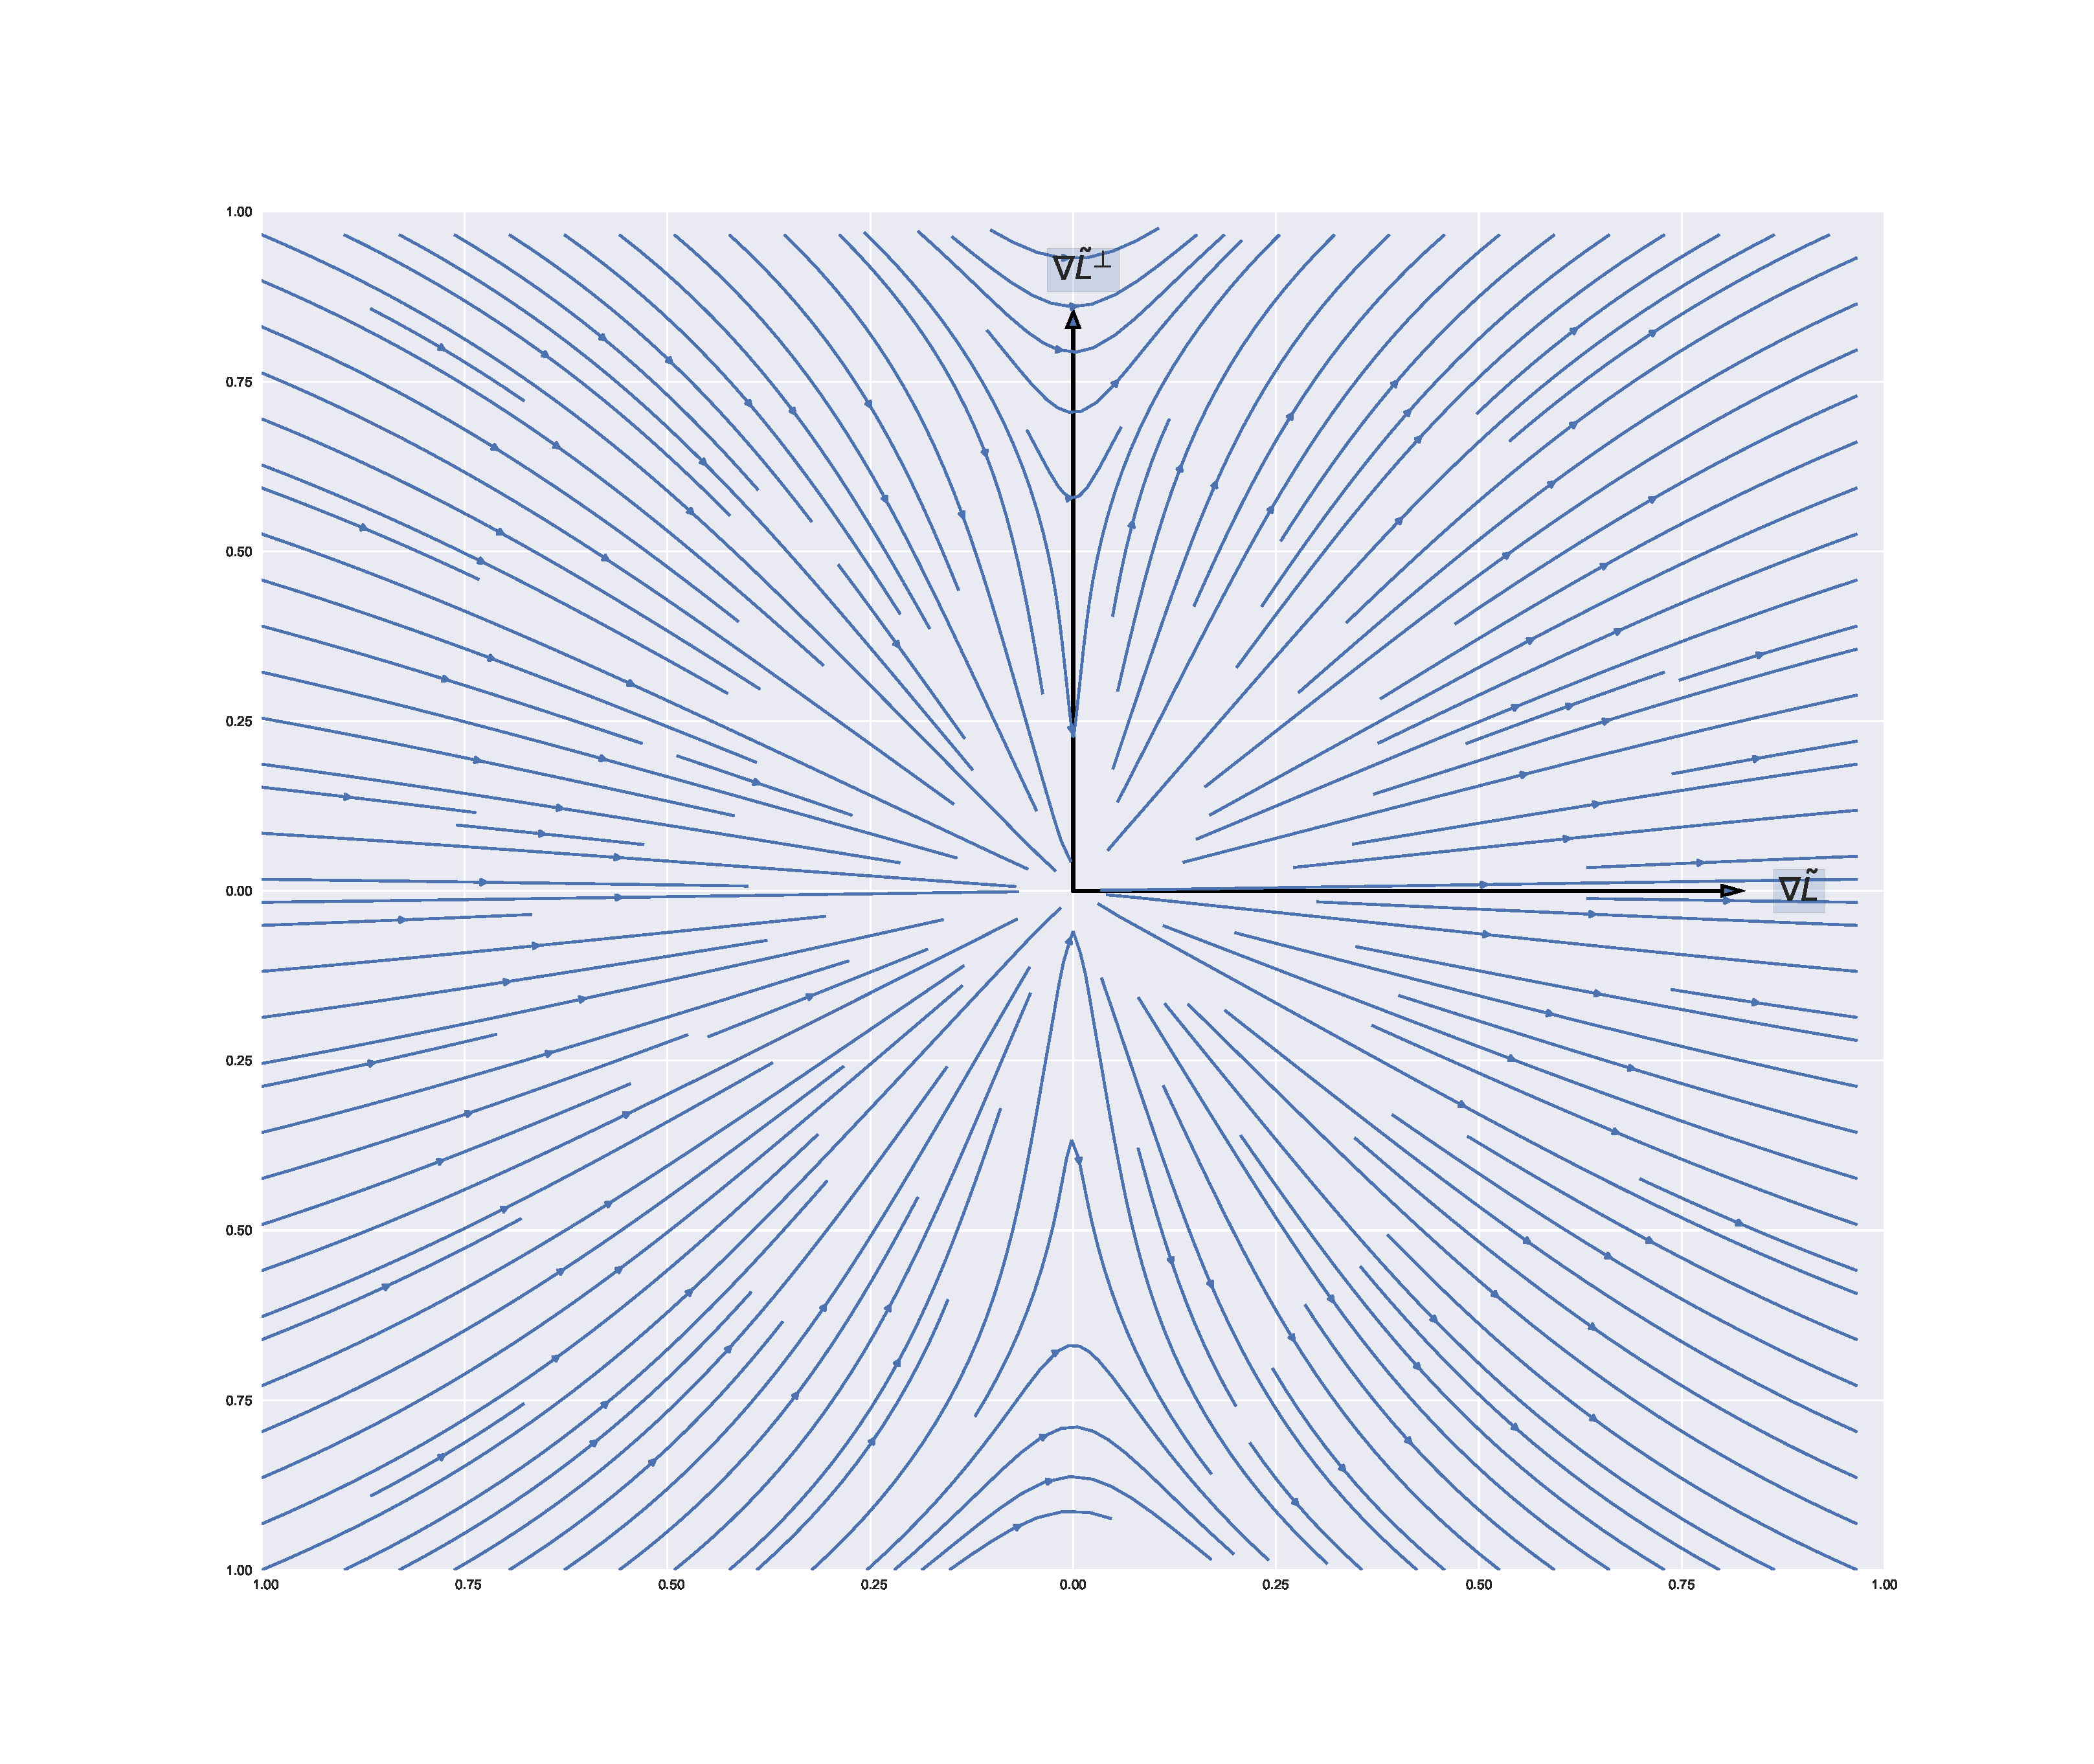
\includegraphics[width=\linewidth]{figures/dynamics_delta_-1.pdf}
    % \endminipage\hfill
    \minipage{0.33\textwidth}
    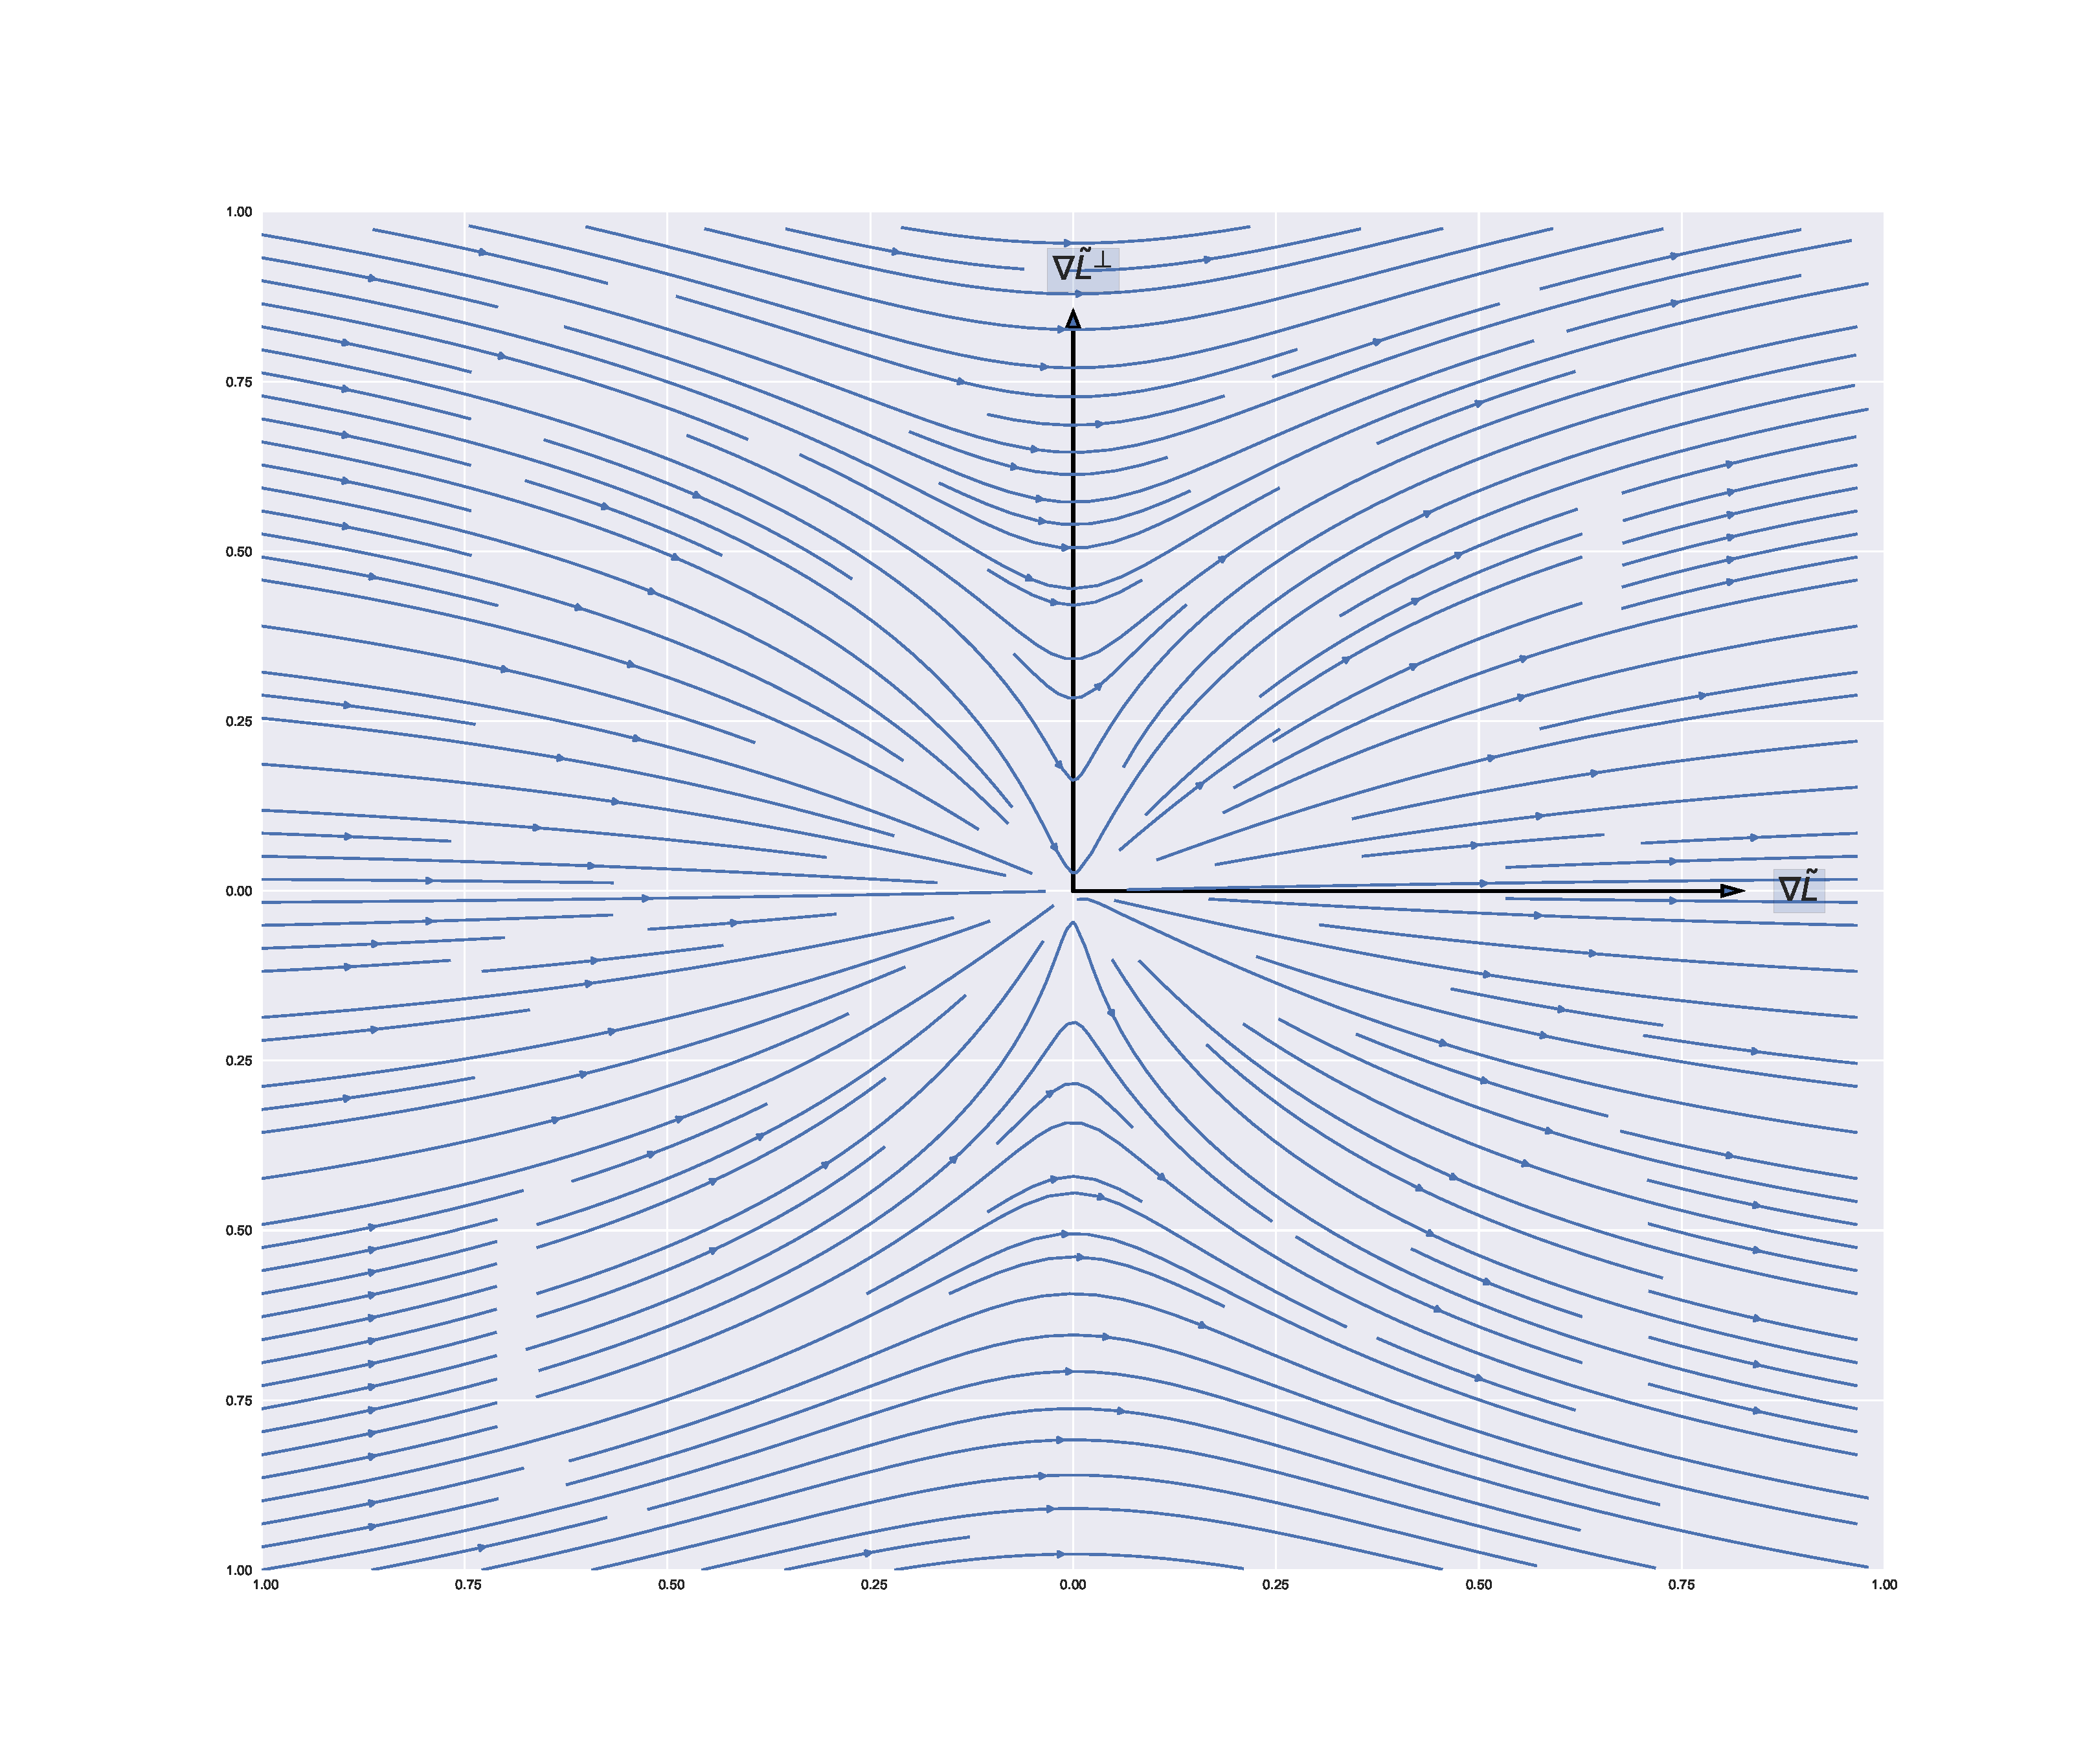
\includegraphics[width=\linewidth]{figures/dynamics_delta_0.pdf}
    \endminipage\hfill
    % \minipage{0.2\textwidth}
    % 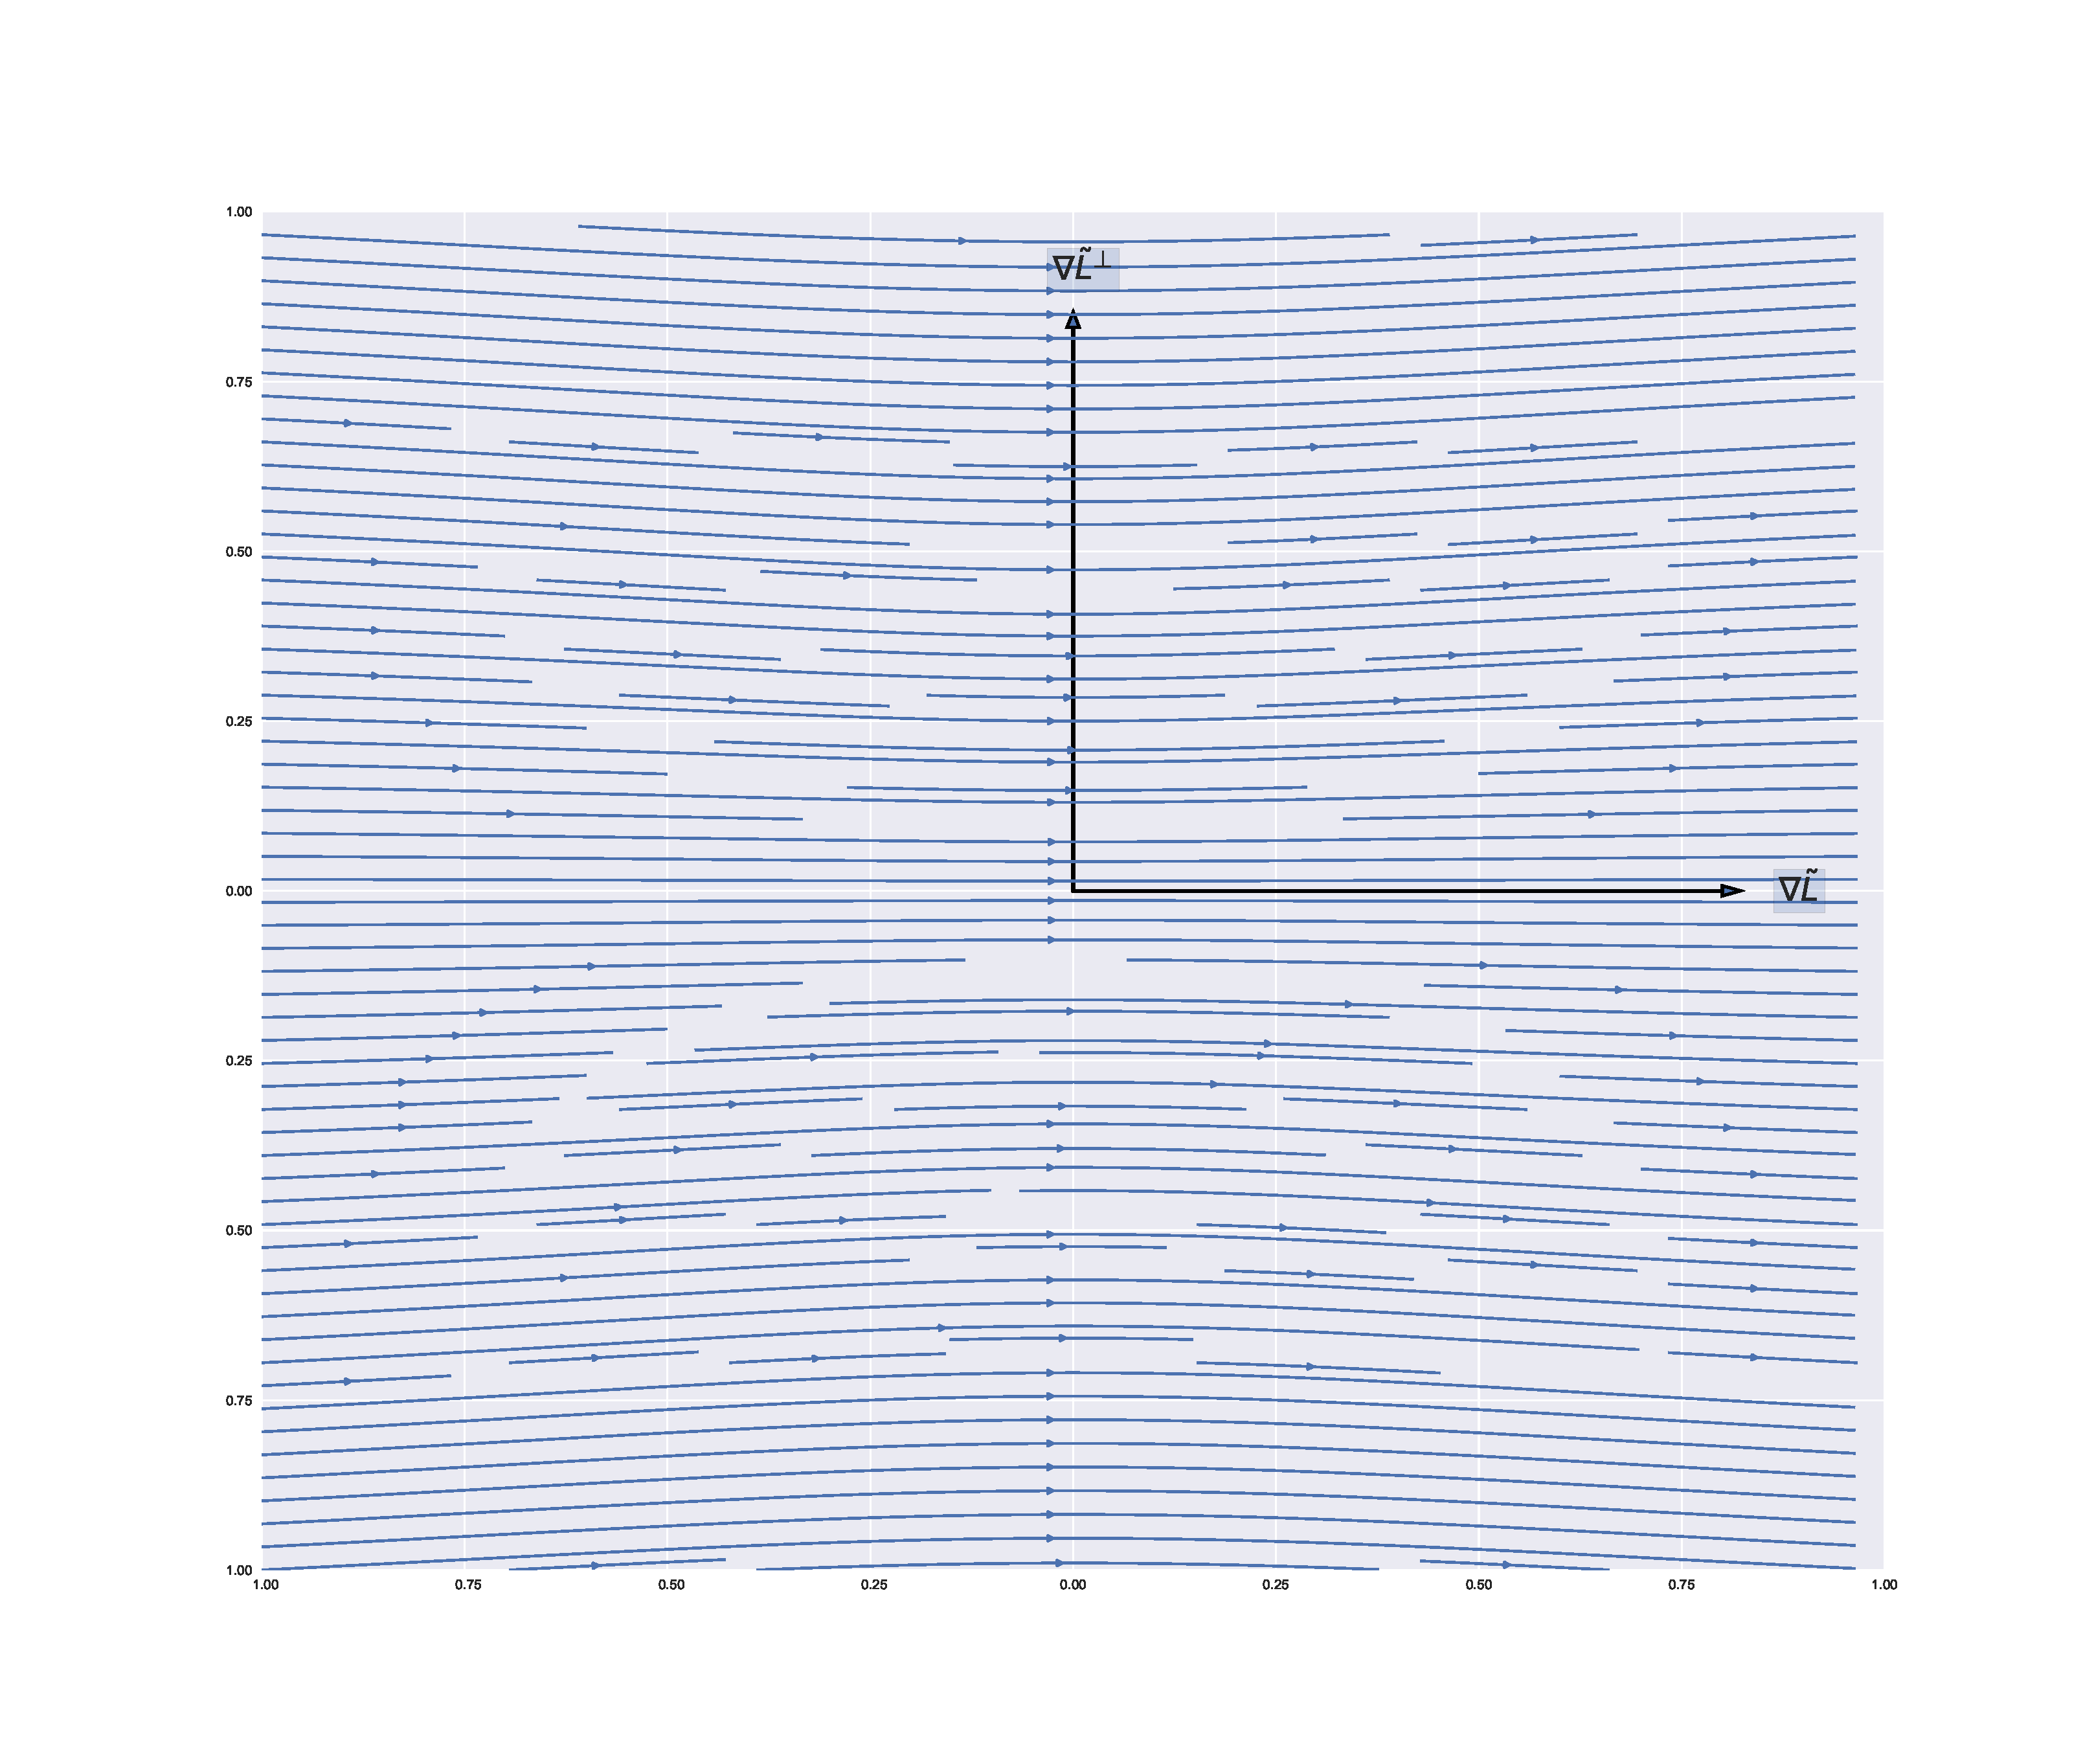
\includegraphics[width=\linewidth]{figures/dynamics_delta_1.pdf}
    % \endminipage\hfill
    \minipage{0.33\textwidth}
    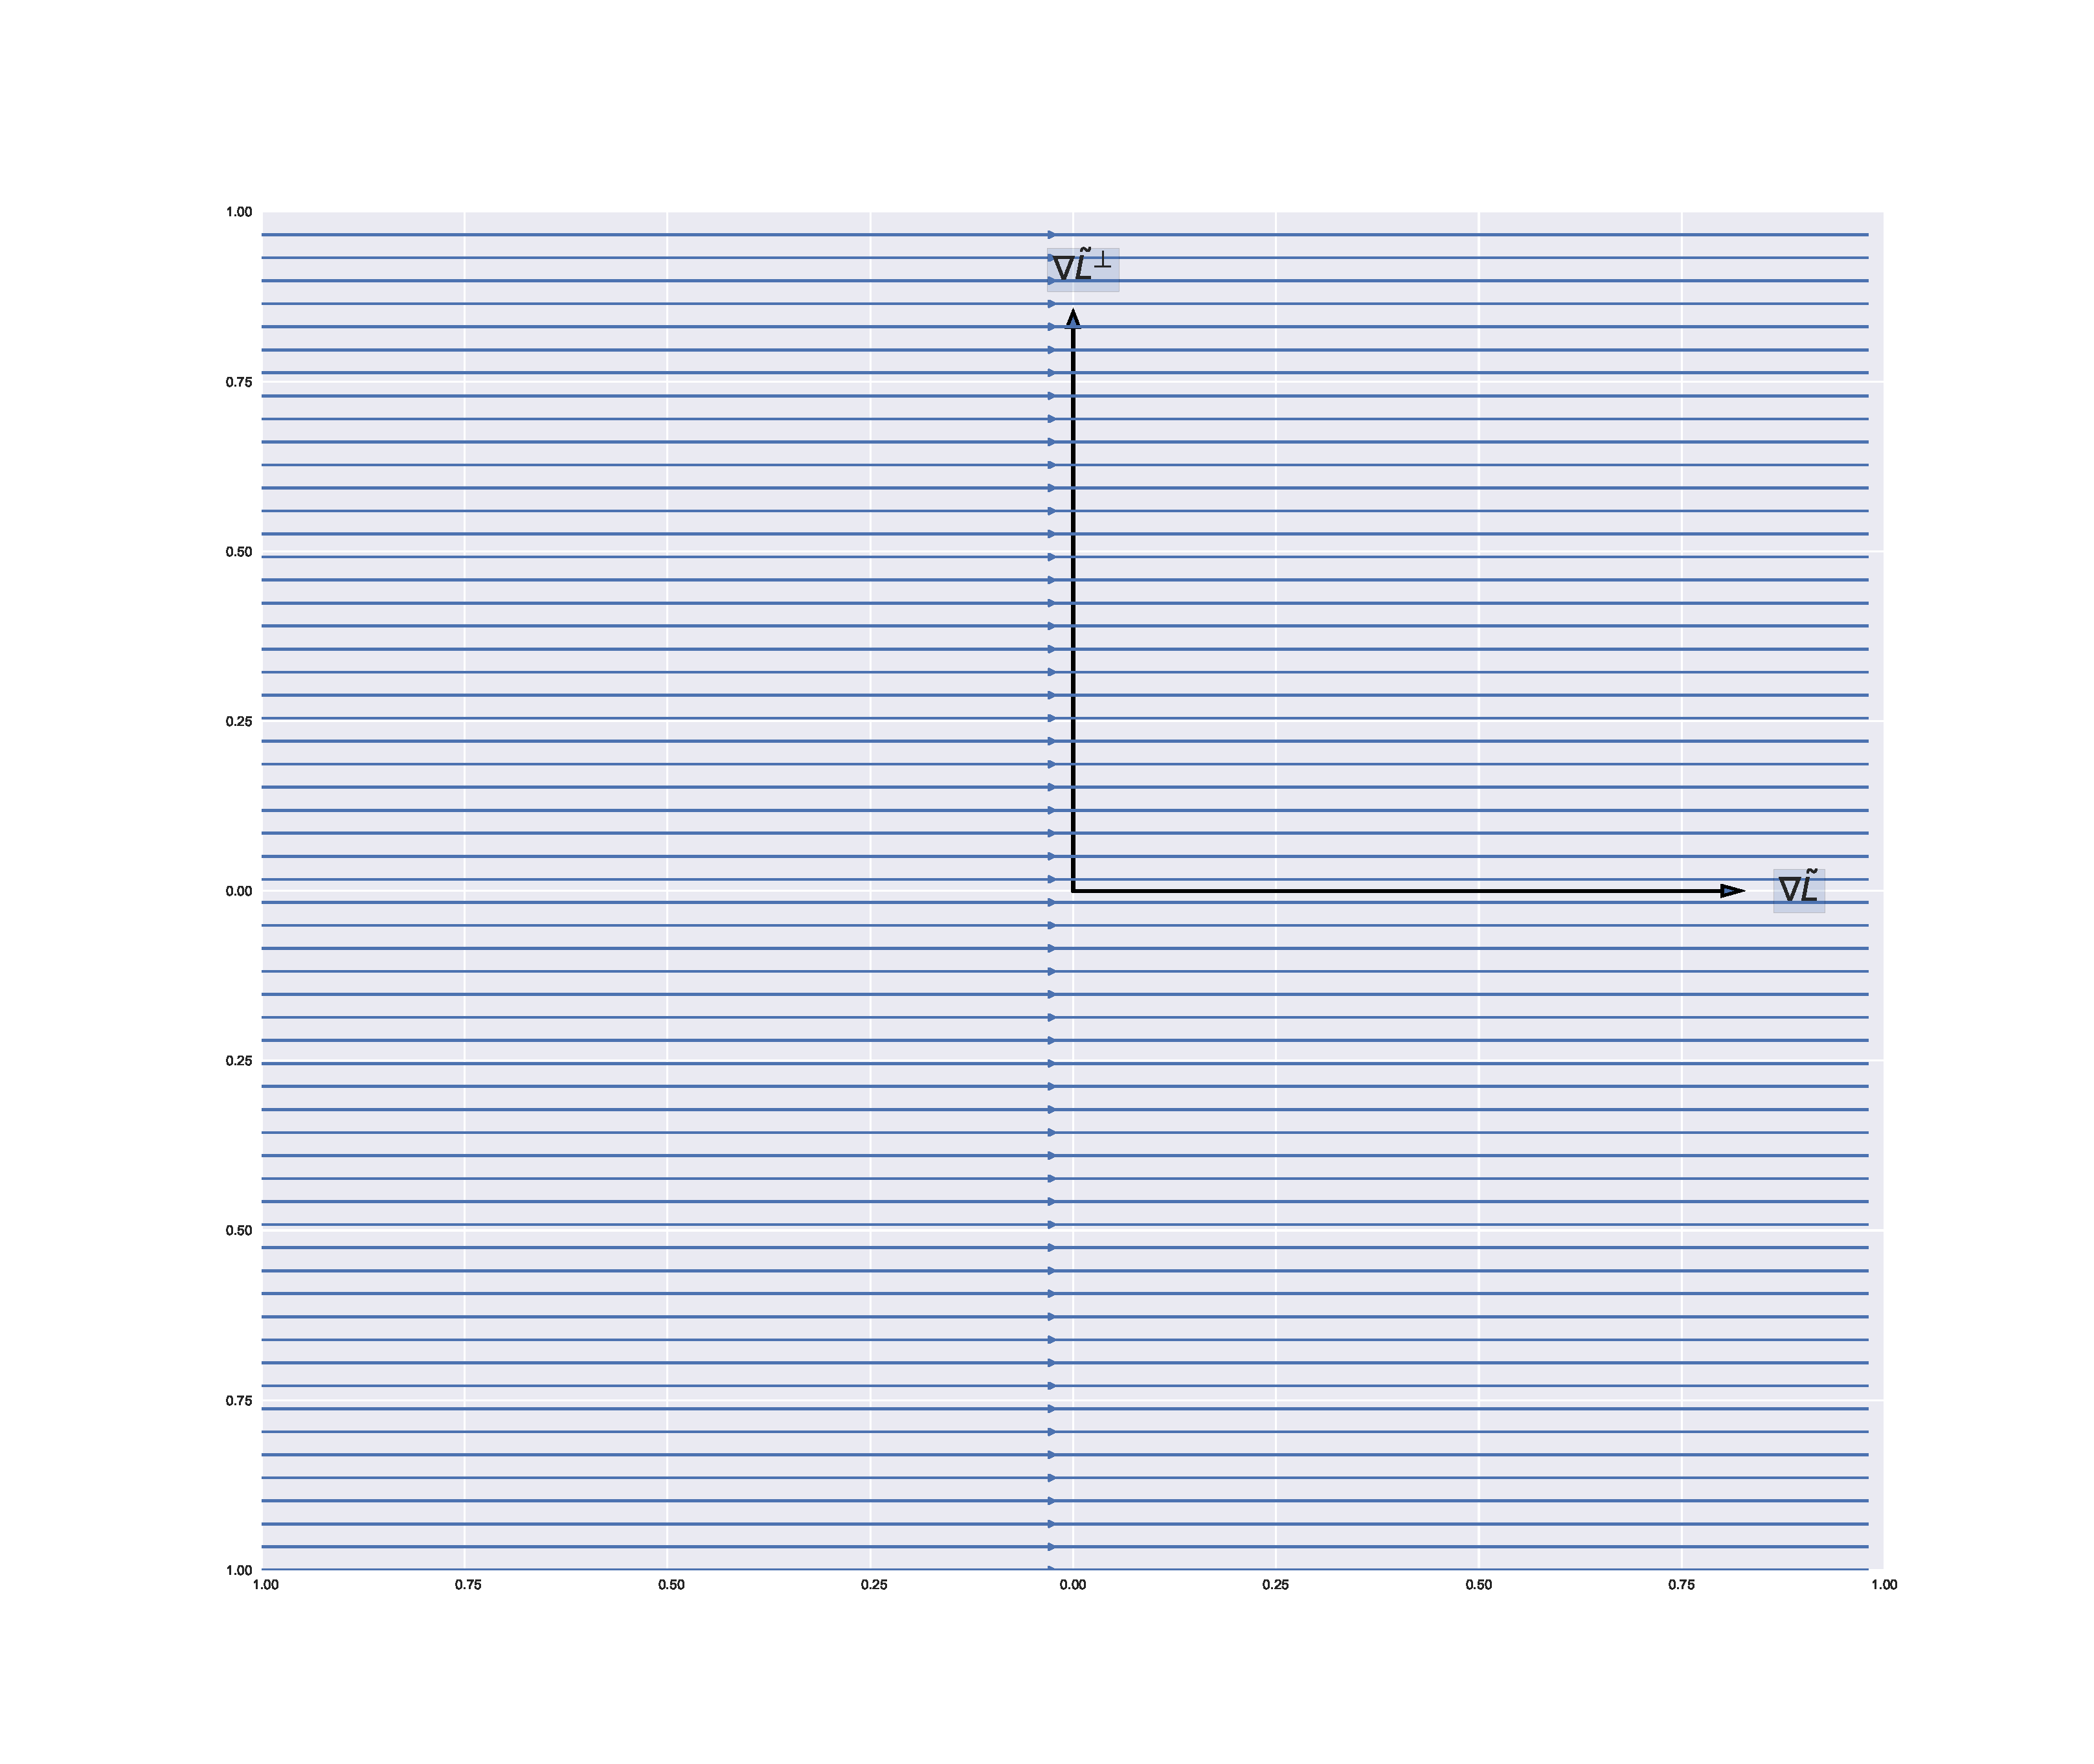
\includegraphics[width=\linewidth]{figures/dynamics_delta_100.pdf}
    \endminipage
    
    \caption{The value of $\delta$ interpolates between different kinds of local trajectories of neurons. The plots are in the coordinate frame $(\nabla \tilde{L}, \nabla \tilde{L}^\bot)$. The left shows $\delta = -100$, in this case, the neurons move radially towards and away from the origin. The middle image shows the trajectories for $\delta = 0$ which has trajectories containing both radial and tangential components. The right image shows the trajectories for $\delta = 100$ which are parallel to the gradient $\nabla \tilde{L}$.}
    \label{fig:my_label}
\end{figure}






\section{Numerical Experiments}

\subsection{Cubic Splines}
We compare 
\subsection{Kernel Learning vs Random Feature Kernel}
We verify that for a large number of neurons the random feature Kernel with the default PyTorch initialization $\bm a, \bm b ~ U(-1, 1), \bm c ~ \frac{1}{m}U(0, 1)$.

\subsection{Sweeping Between Adaptive and Kernel Learning}
We compare different initial parameters, $\bm a, \bm b, \bm c$ which correspond to the same initial function but different values of the conserved quantity $\delta$, sweeping between the kernel and adaptive regimes.


\begin{figure}
    \centering
    \minipage{0.33\textwidth}
    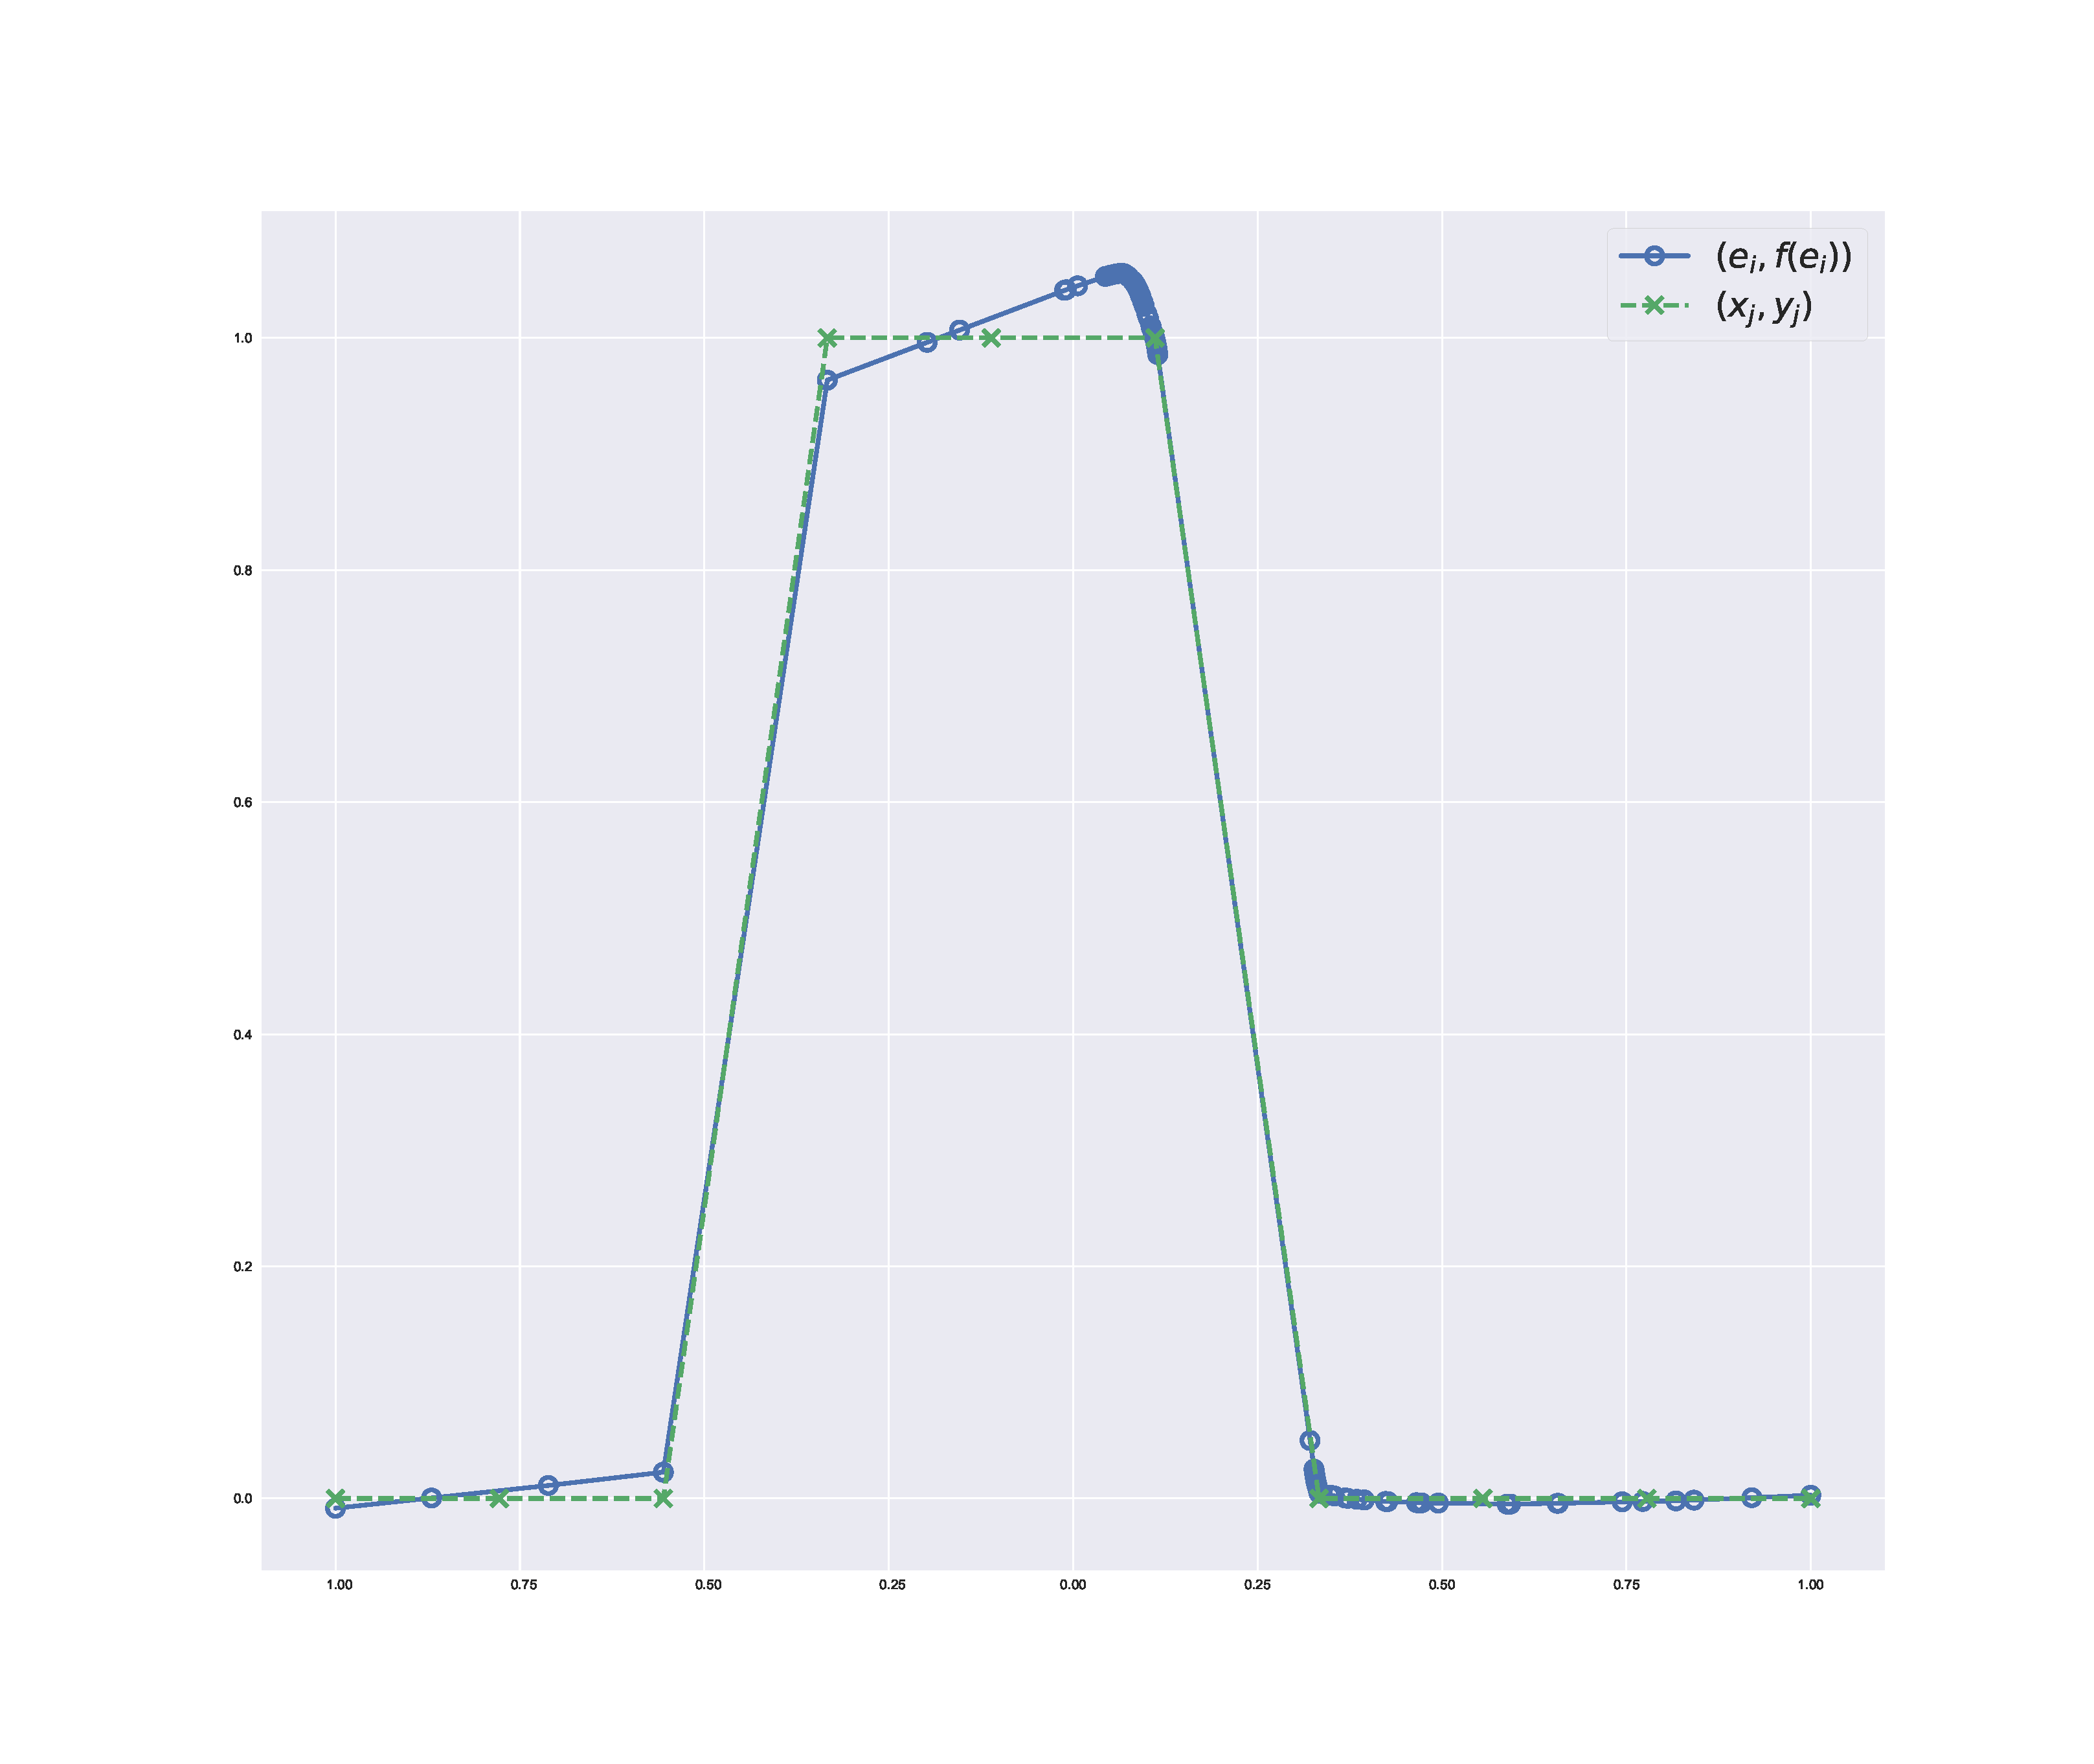
\includegraphics[width=\linewidth]{figures/neuron_trajectories_recon.pdf}
    \endminipage\hfill
    \minipage{0.33\textwidth}
    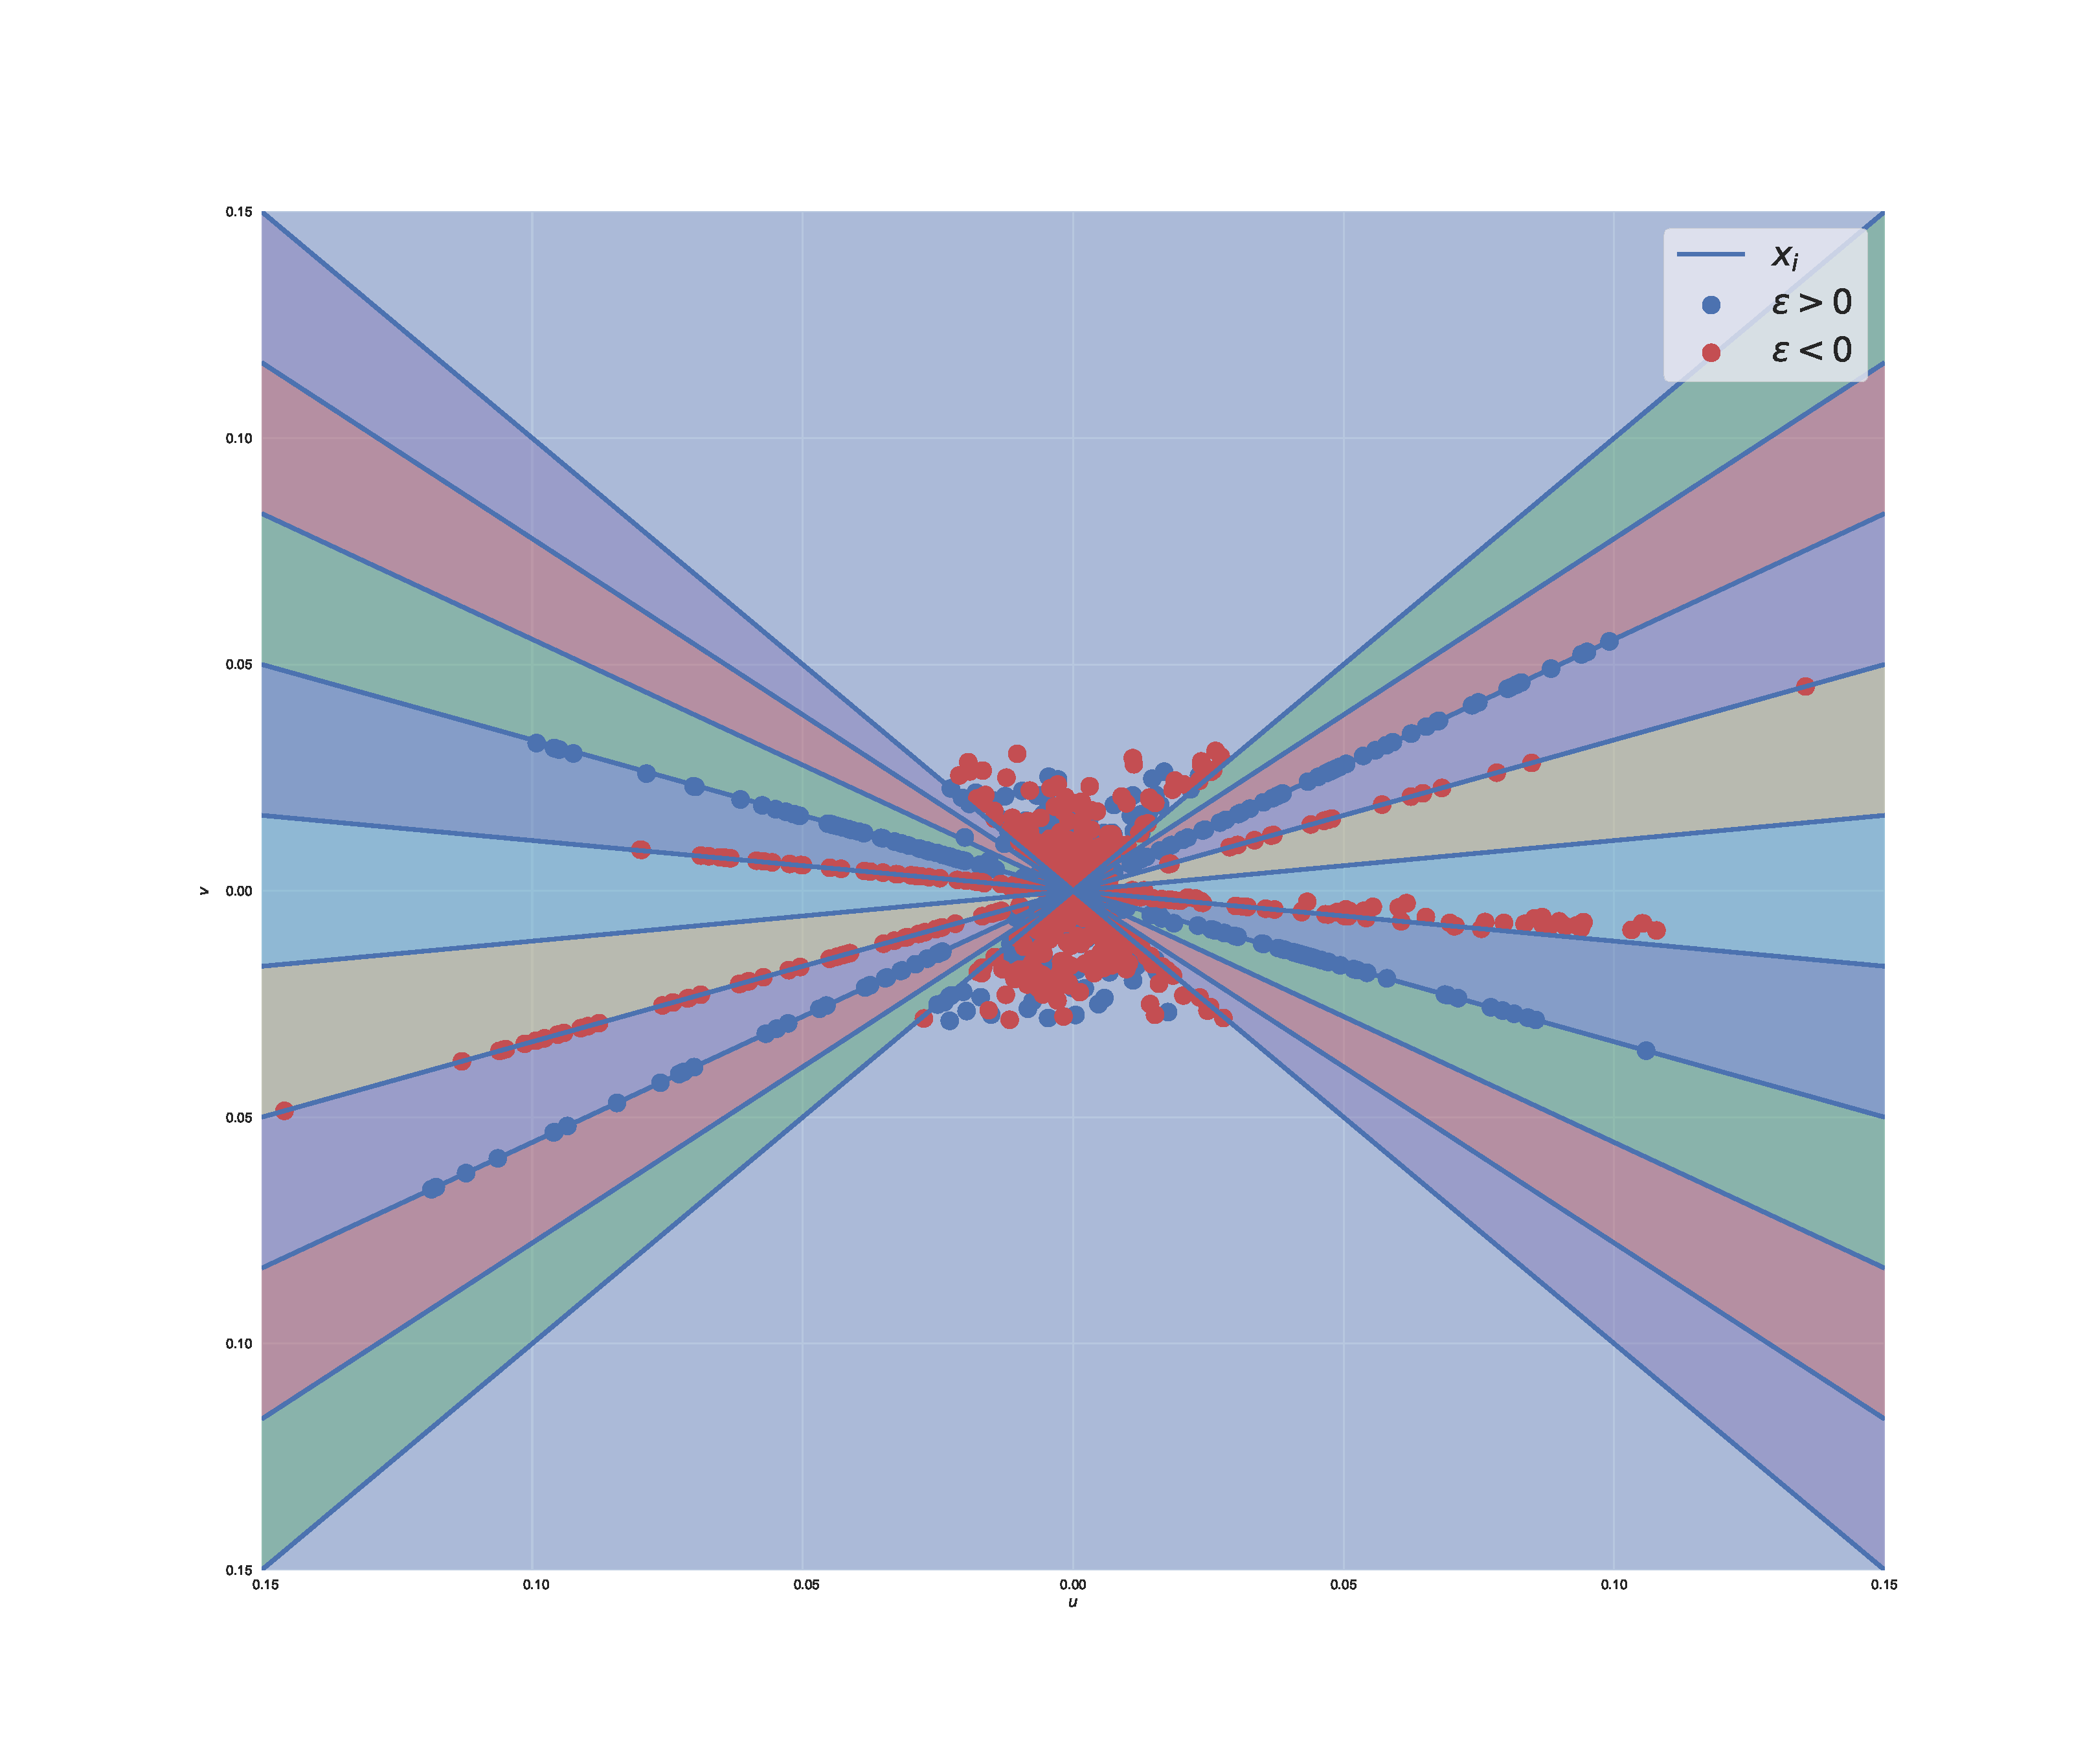
\includegraphics[width=\linewidth]{figures/neuron_trajectories_phase.pdf}
    \endminipage\hfill
    \minipage{0.33\textwidth}
    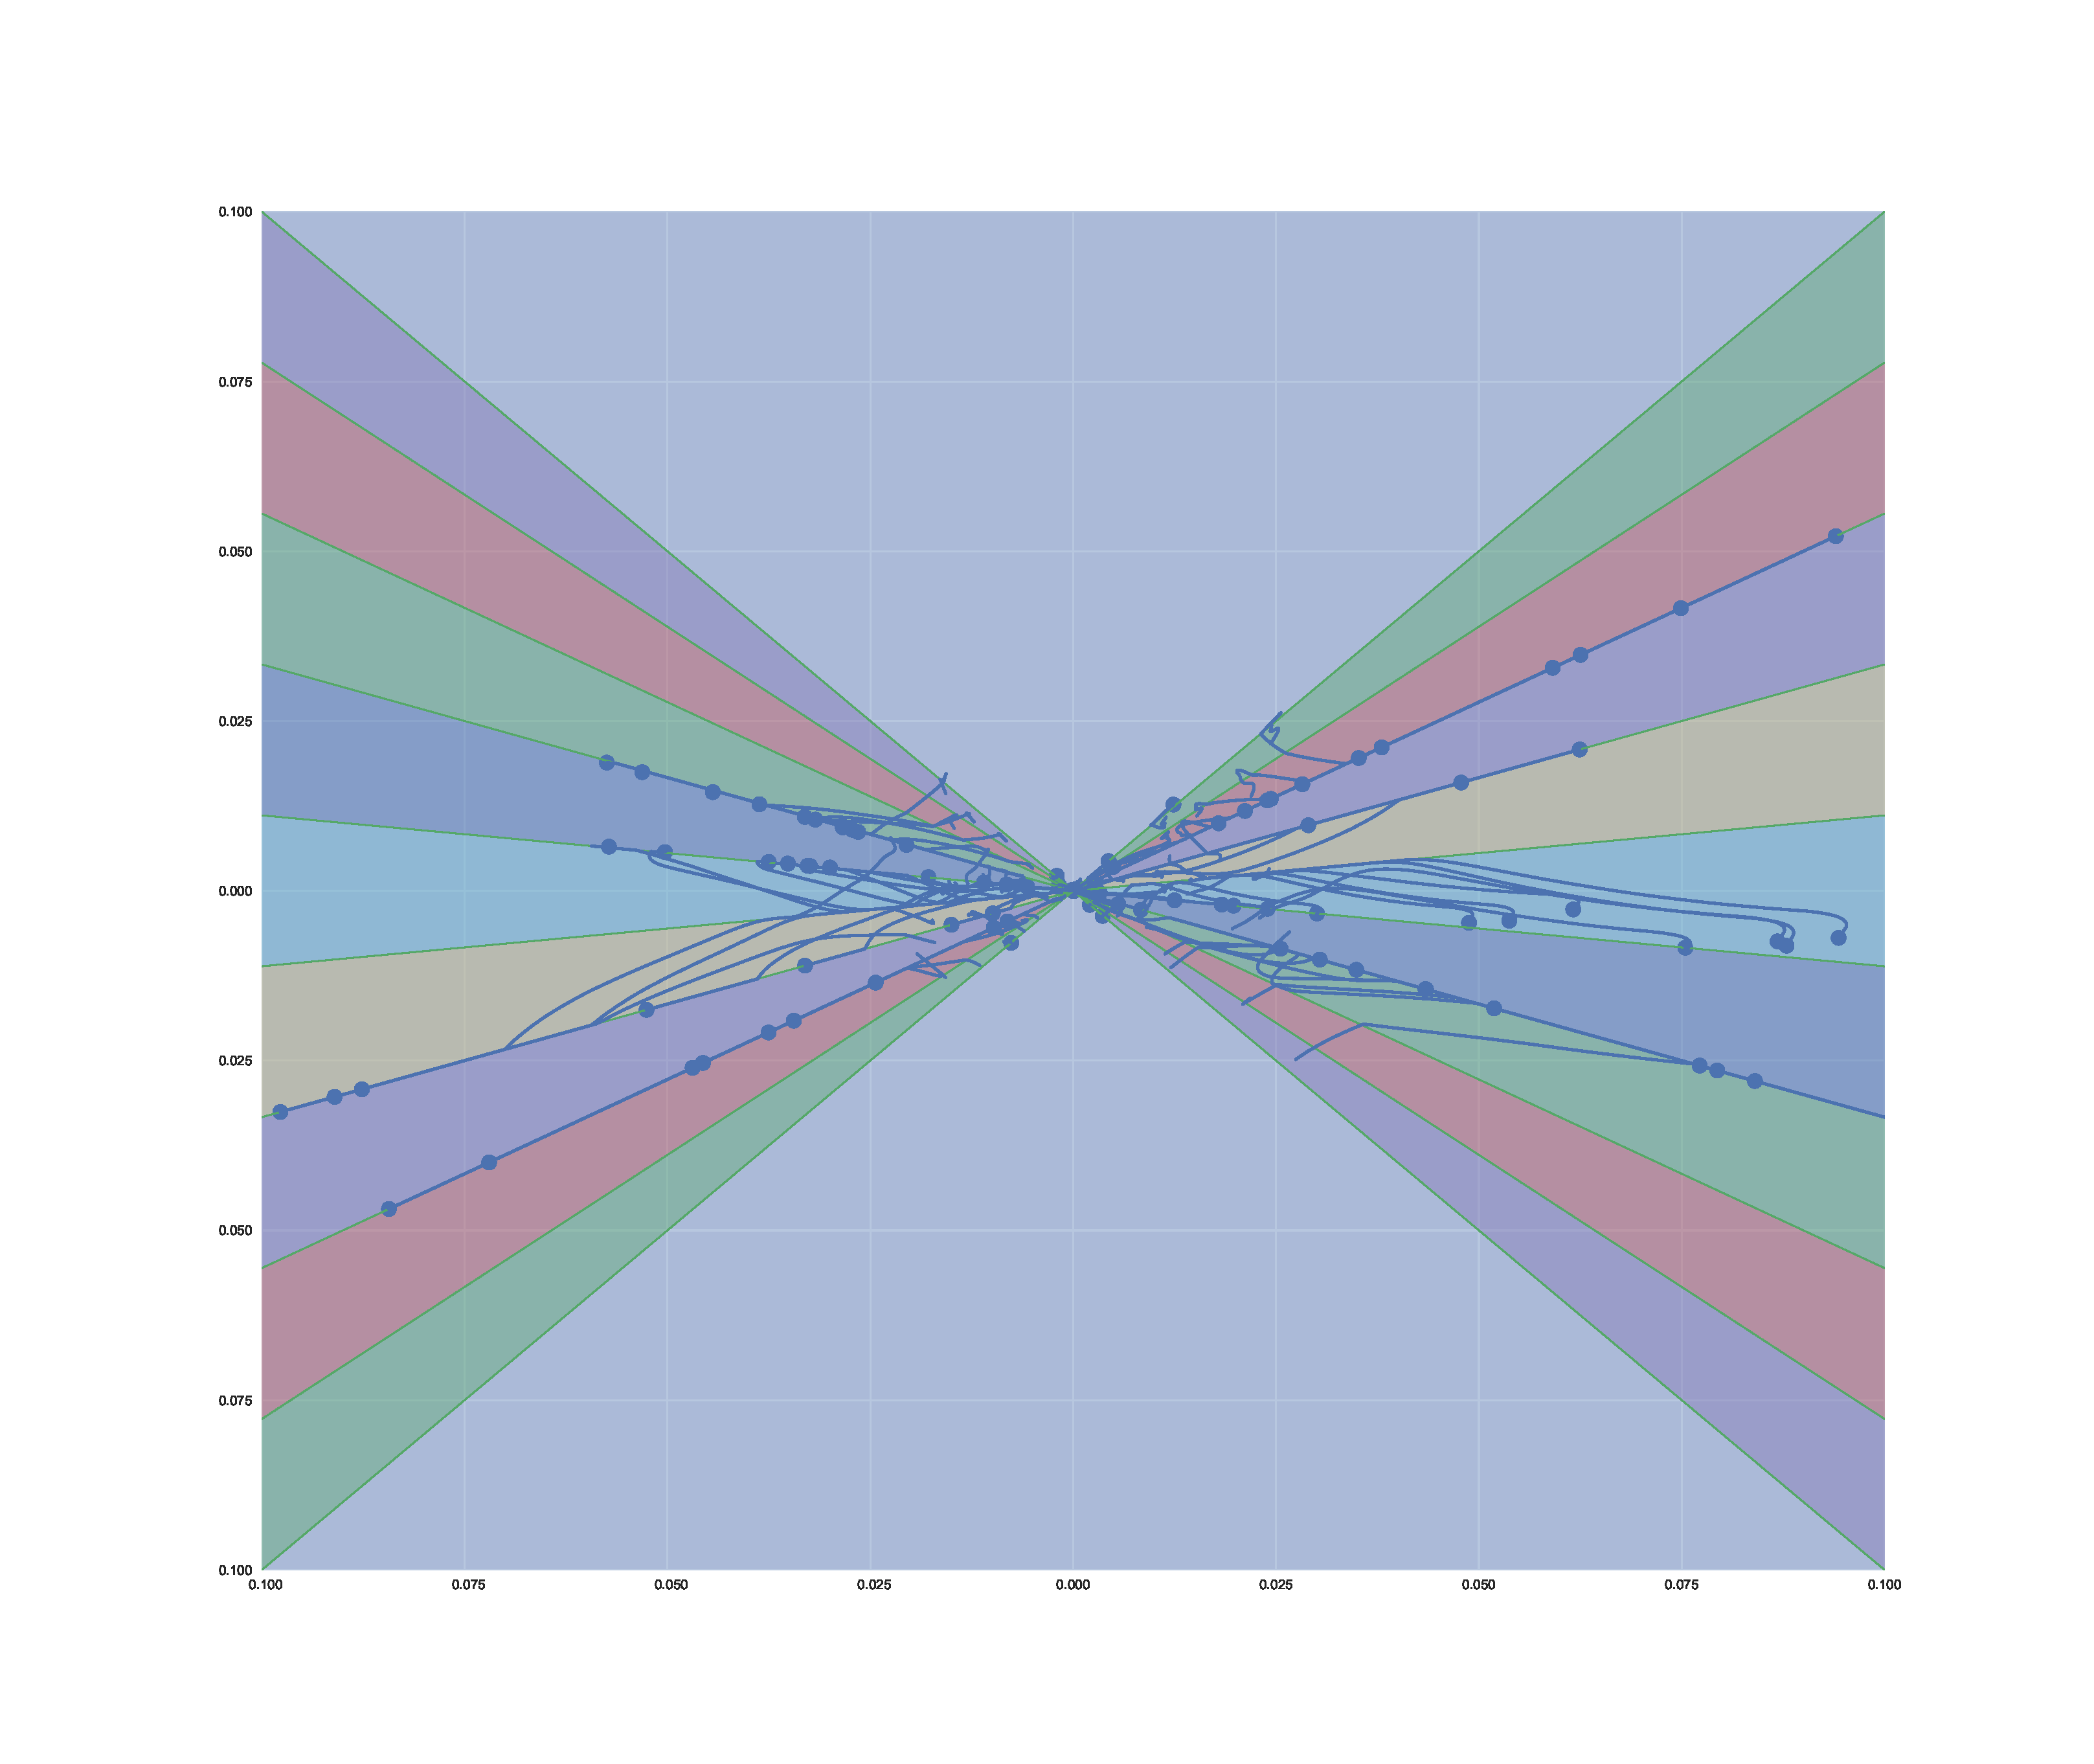
\includegraphics[width=\linewidth]{figures/neuron_trajectories.pdf}
    \endminipage
    \caption{Evolution of neurons in the tangential regime while fitting a square wave with 1000 neurons. The left image shows the trained network on and sample points. The middle image shows the distribution of all neurons at the end of training. The right image shows trajectories for a random sample of 100 neurons. Observe how in this regime, neurons concentrate on certain samples. The trajectories in this case get stuck at the sample boundary.}
    \label{fig:tangential_trajectories}
\end{figure}


\begin{figure}
    \centering
    \minipage{0.33\textwidth}
    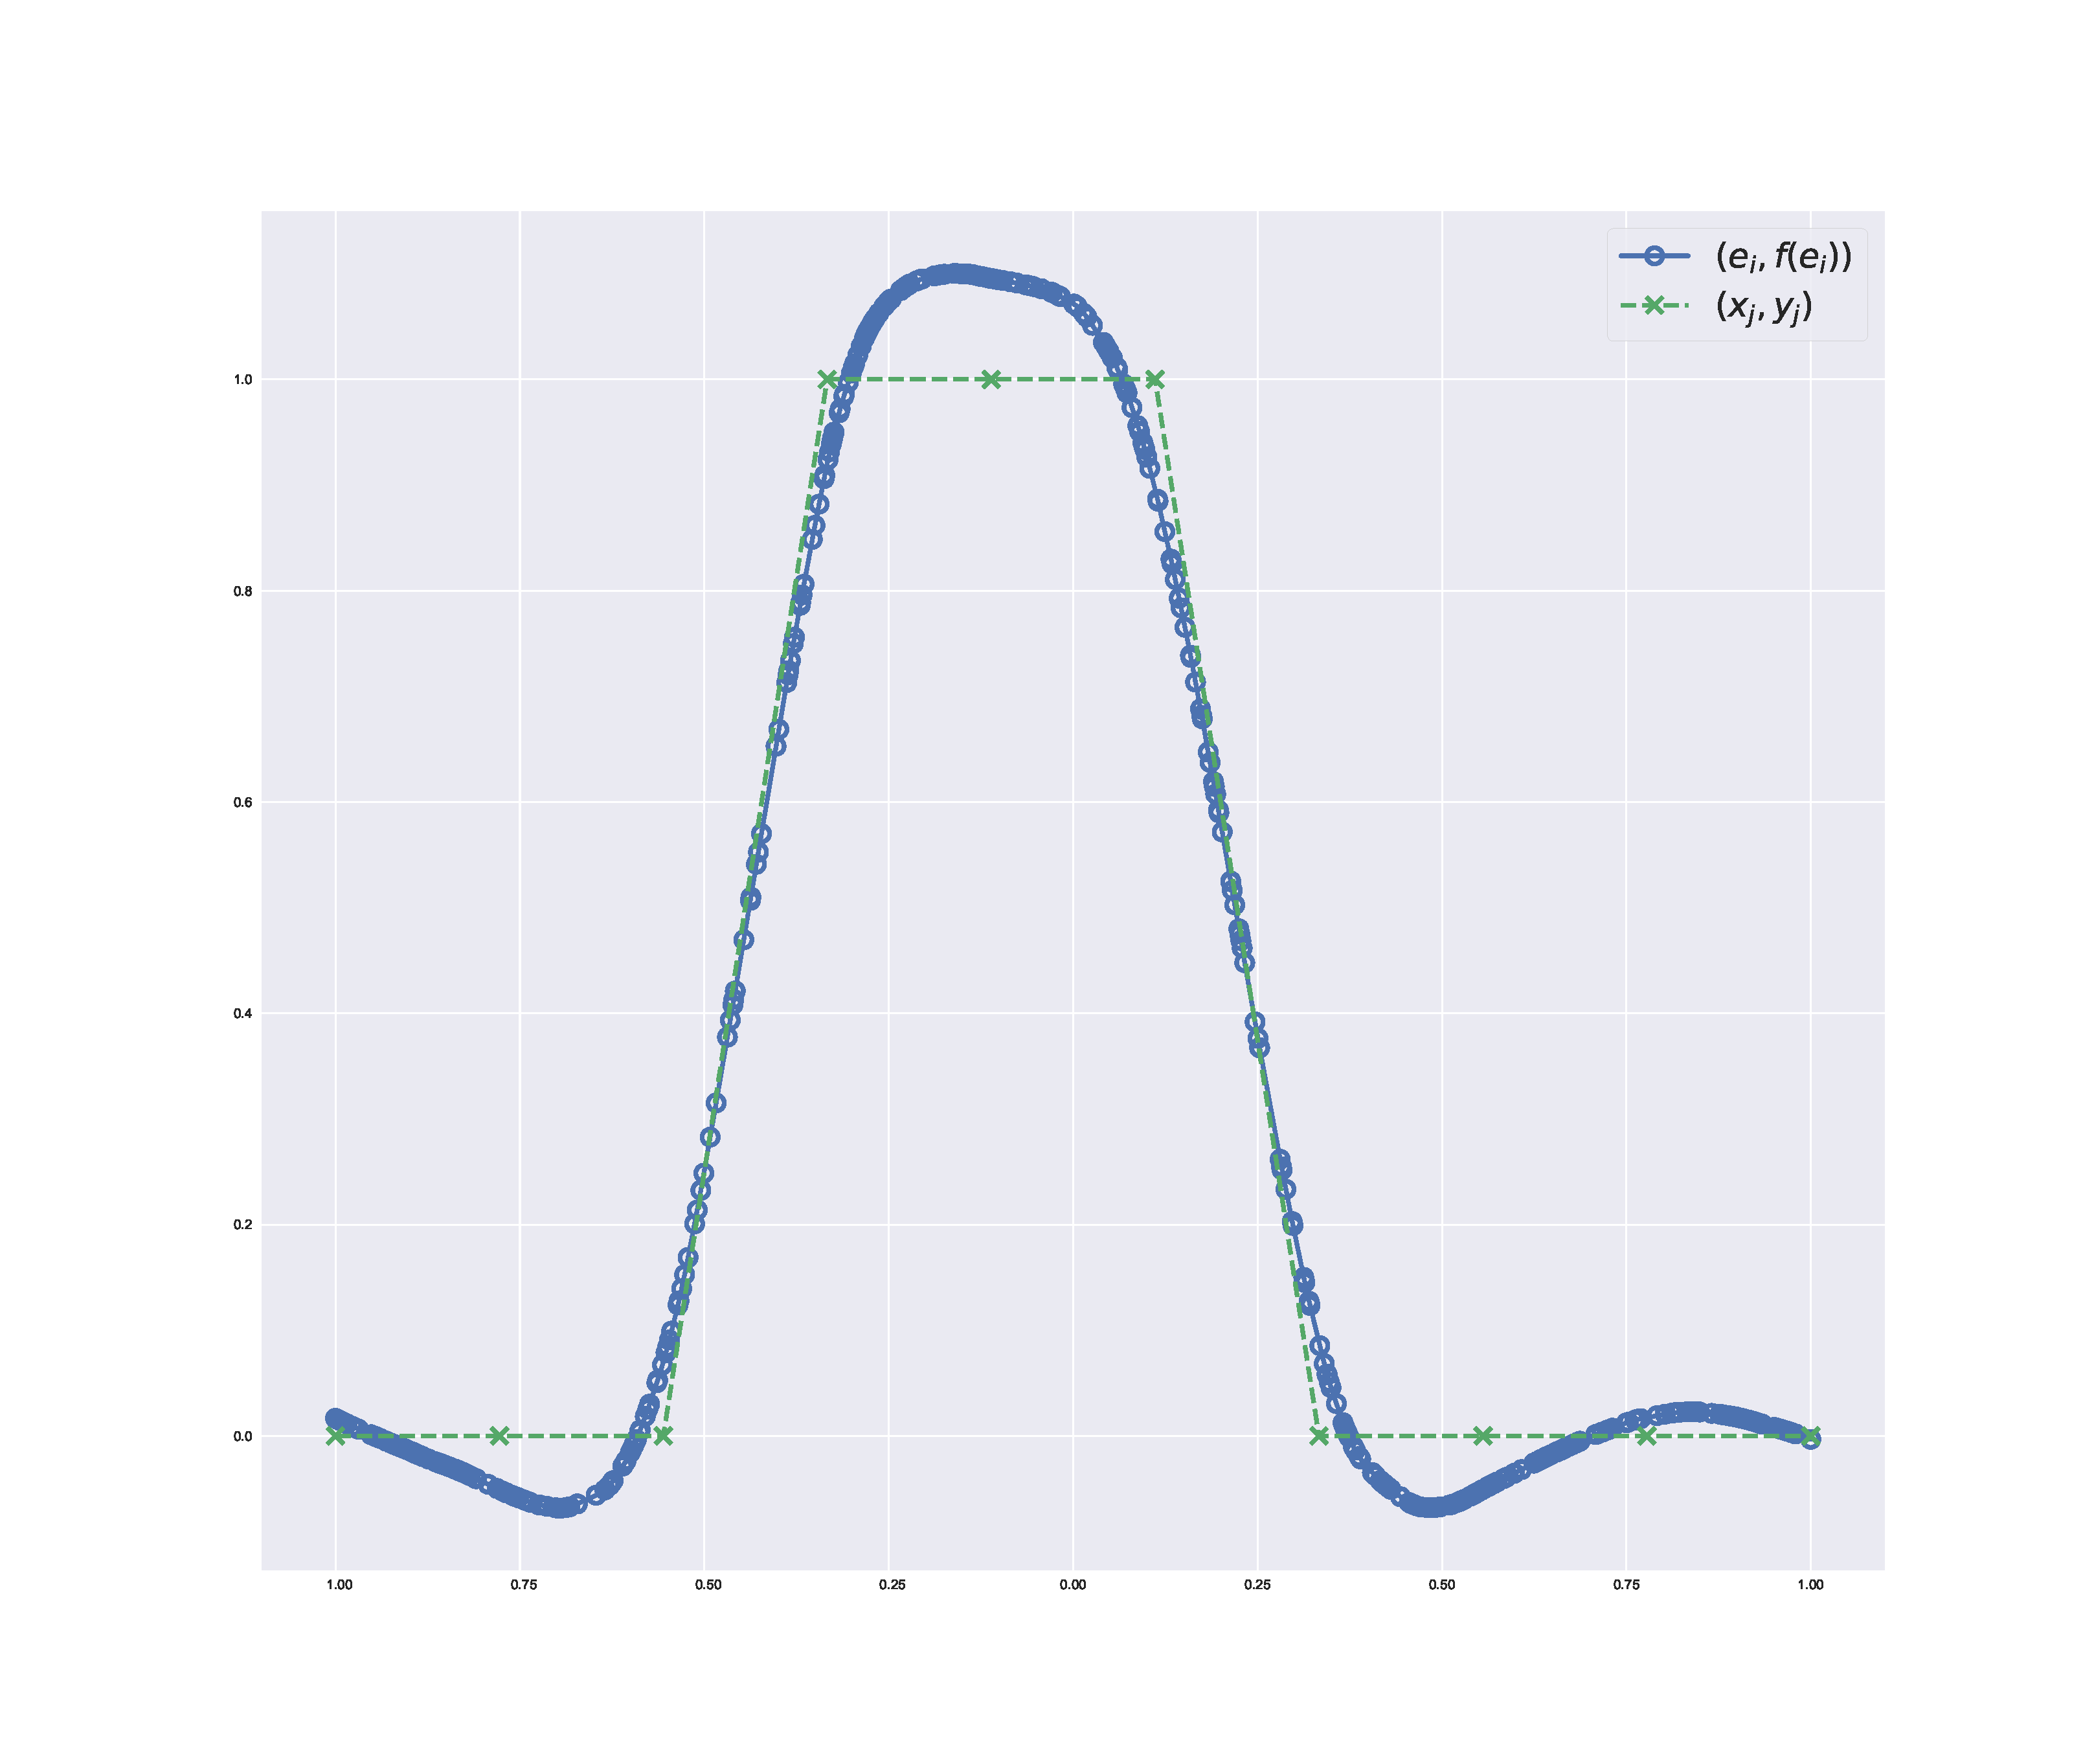
\includegraphics[width=\linewidth]{figures/radial_trajectories_recon.pdf}
    \endminipage\hfill
    \minipage{0.33\textwidth}
    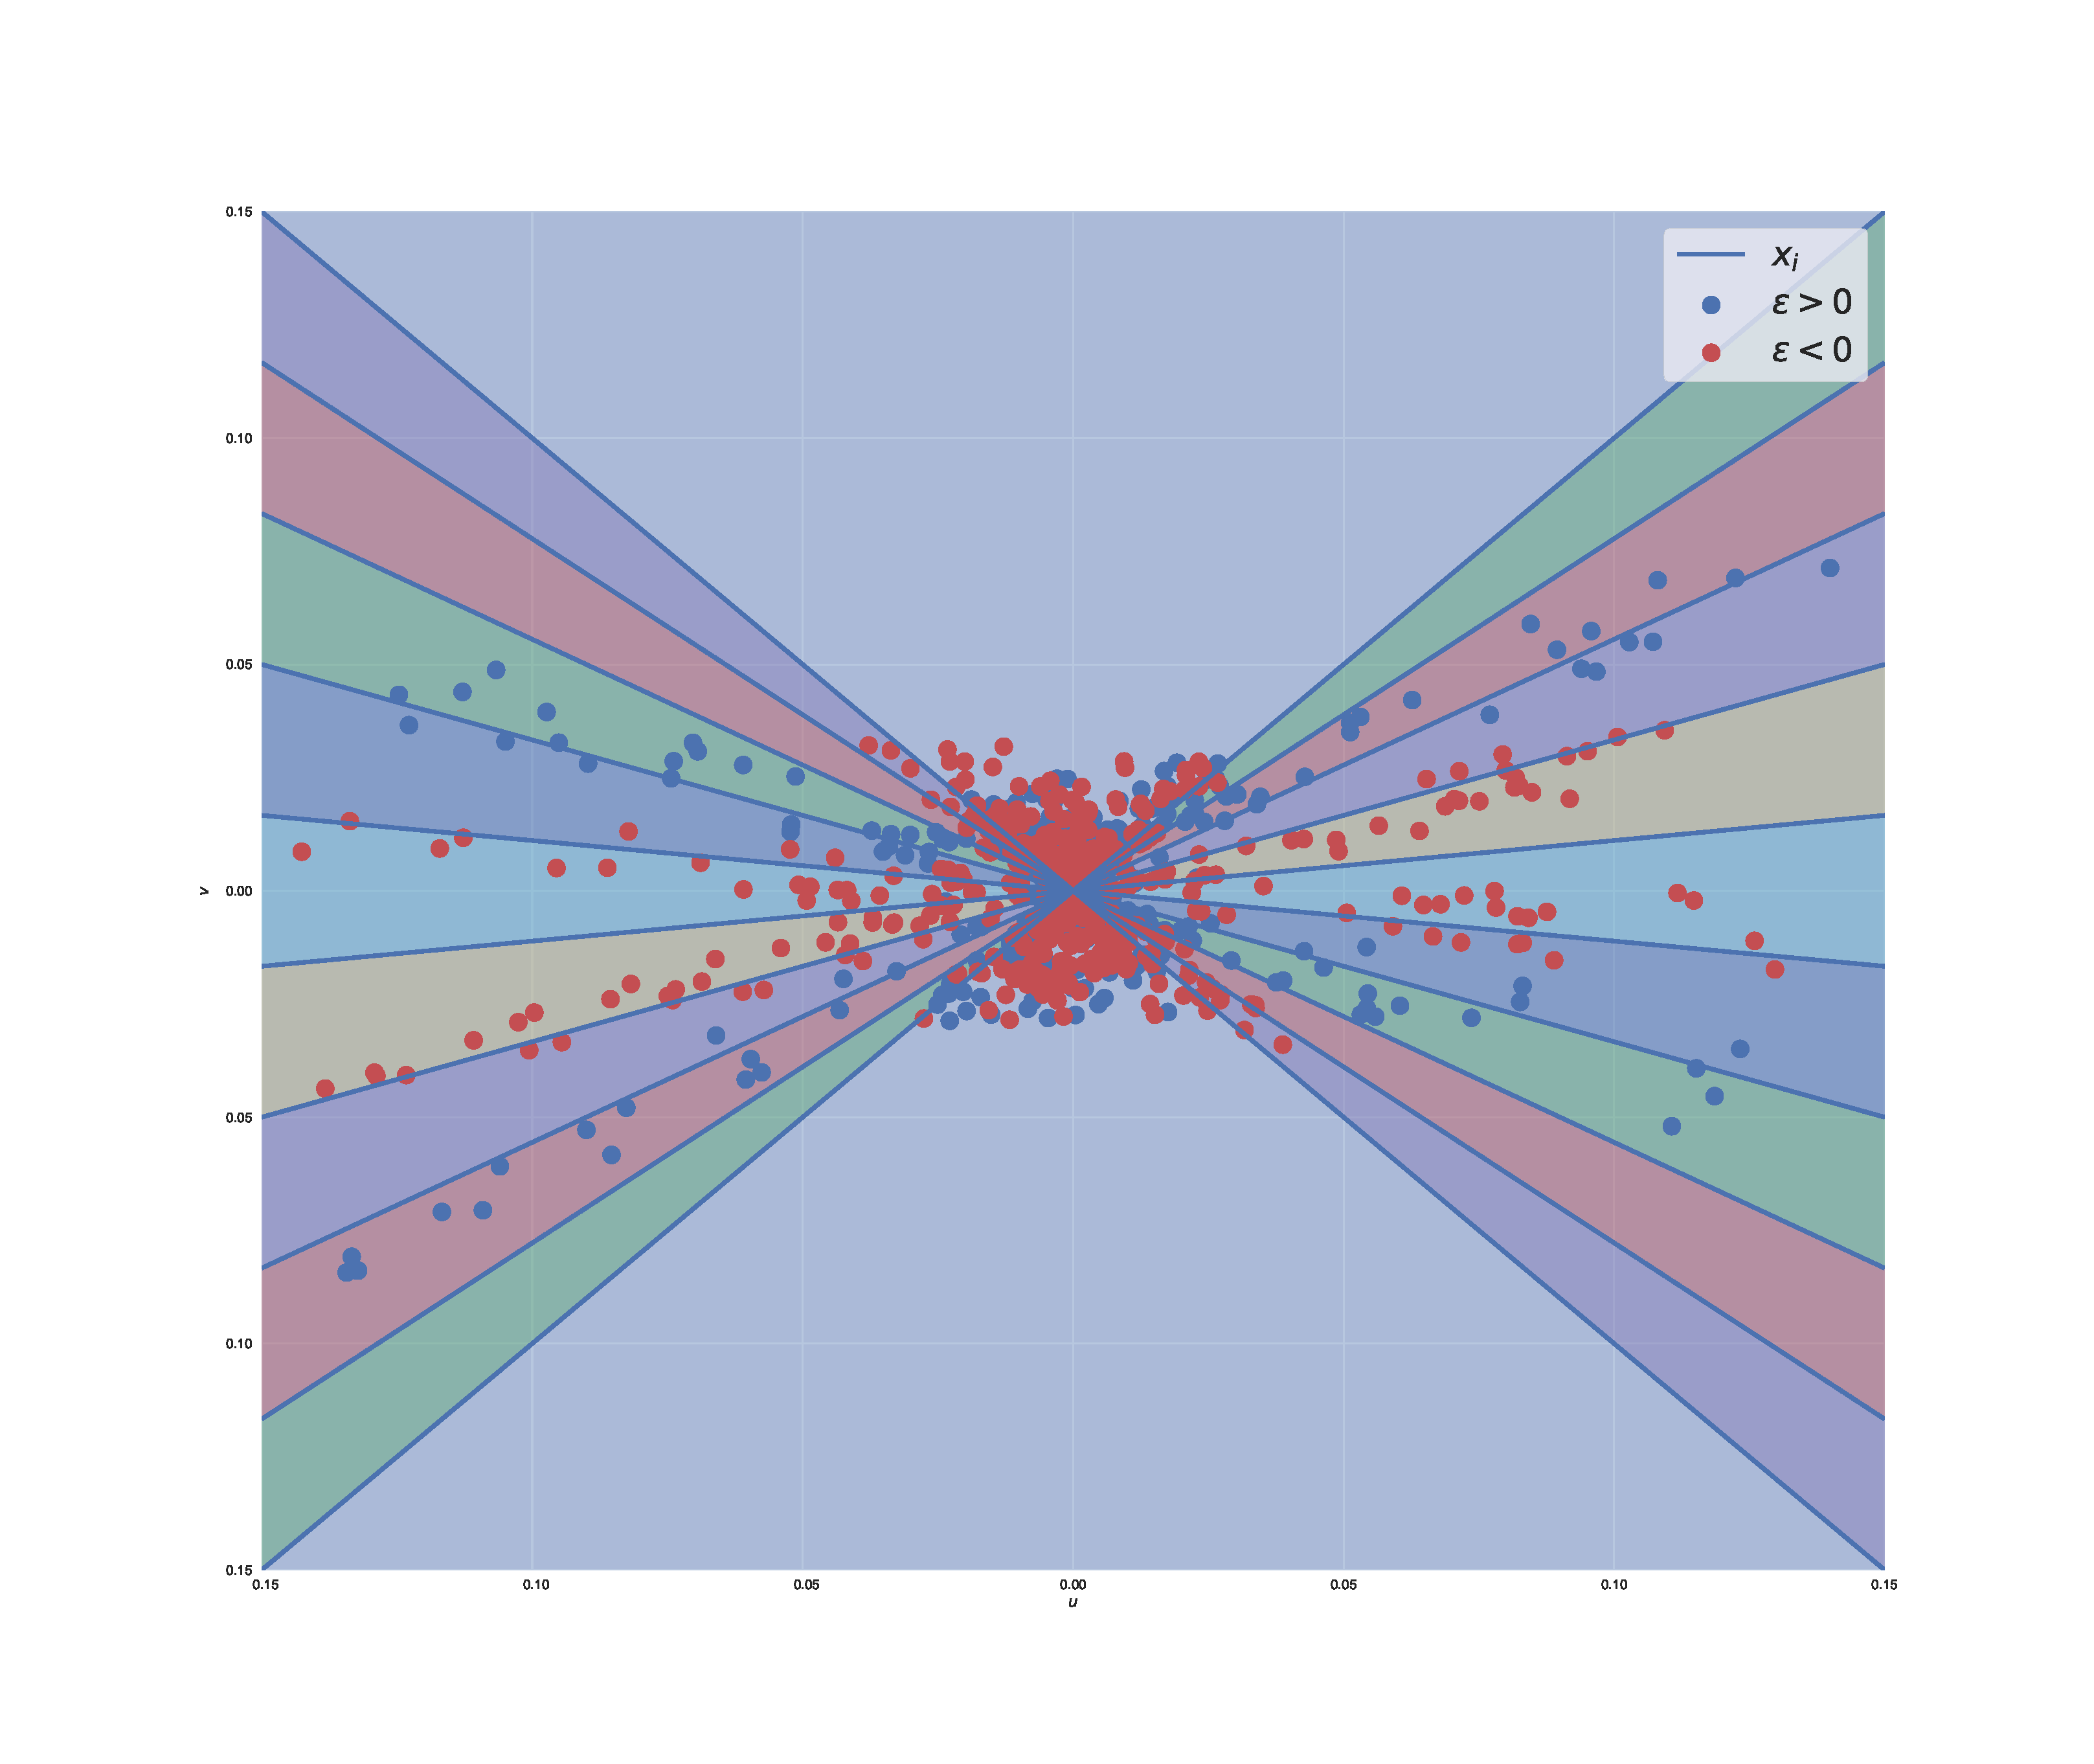
\includegraphics[width=\linewidth]{figures/radial_trajectories_phase.pdf}
    \endminipage\hfill
    \minipage{0.33\textwidth}
    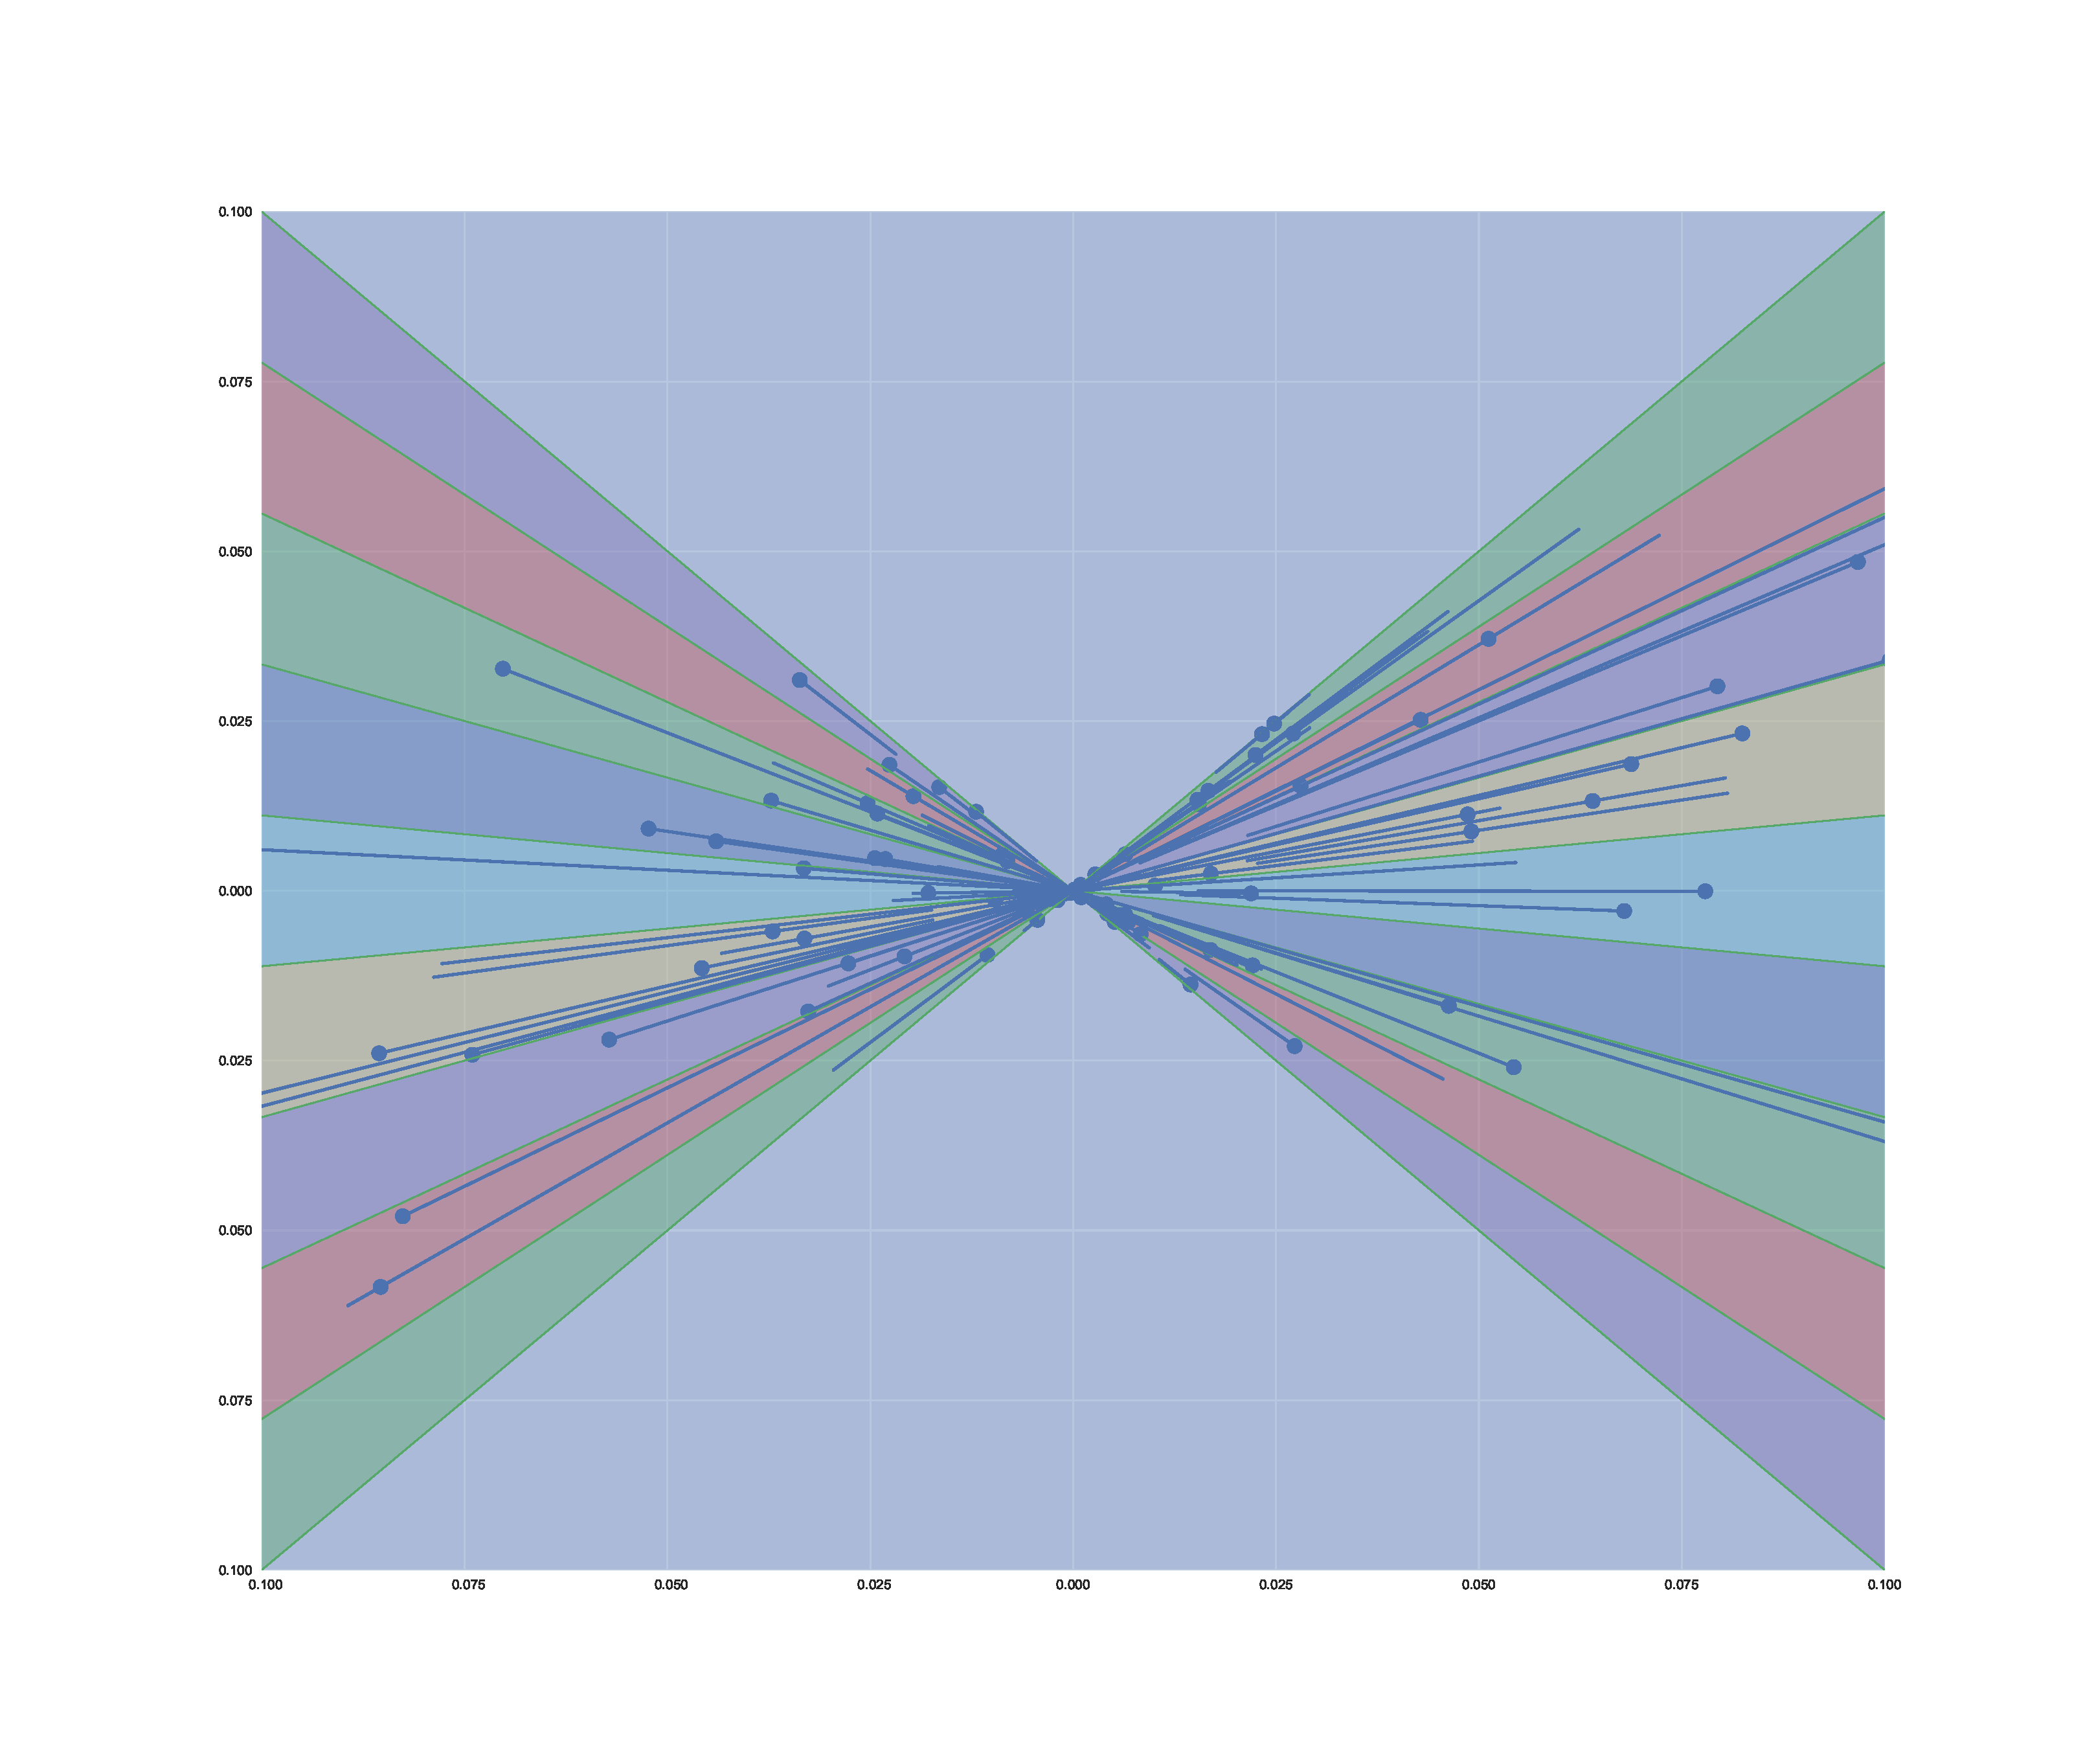
\includegraphics[width=\linewidth]{figures/radial_trajectories.pdf}
    \endminipage
    \caption{Evolution of neurons in the radial regime while fitting a square wave with 1000 neurons. The left image shows the trained network on and sample points. The middle image shows the distribution of all neurons at the end of training. The right image shows trajectories for a random sample of 100 neurons.}
    \label{fig:radial_trajectores}
\end{figure}


\begin{figure}\label{fig:different_funcs_same_init}
    \centering
    \minipage{0.33\textwidth}
    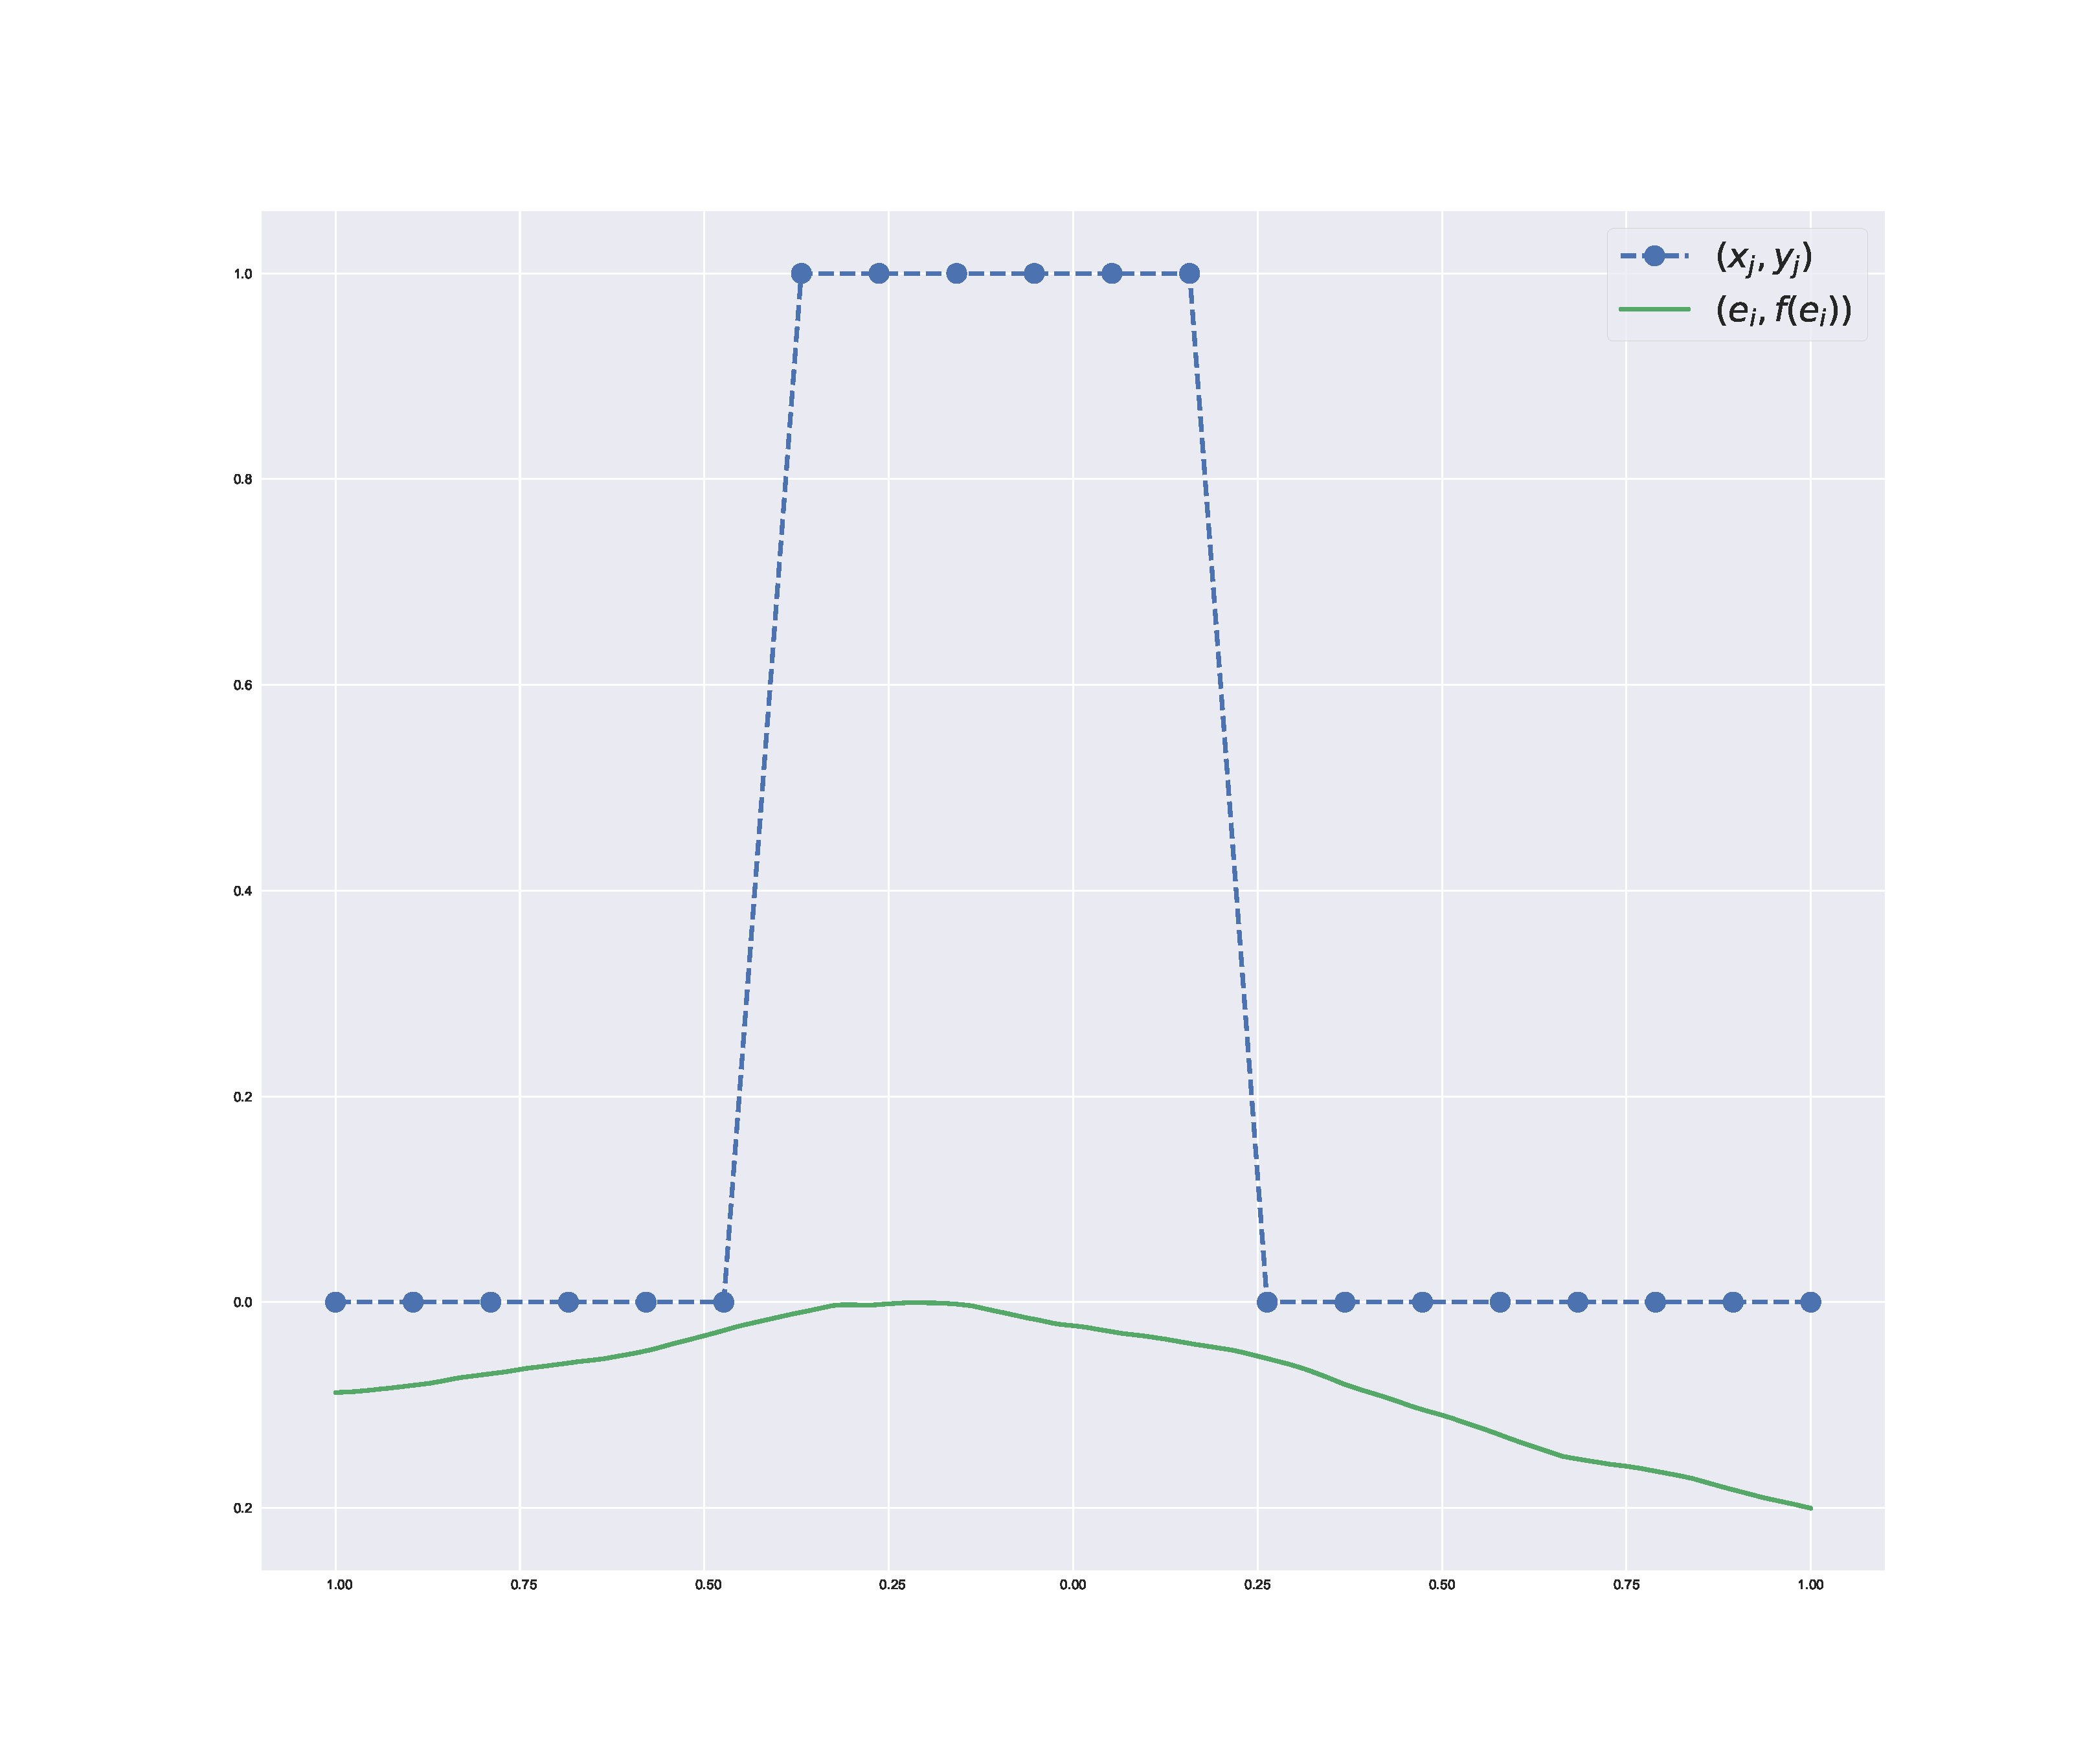
\includegraphics[width=\linewidth]{figures/same_init_different_func_square_init.pdf}
    \endminipage\hfill
    % \minipage{0.2\textwidth}
    % 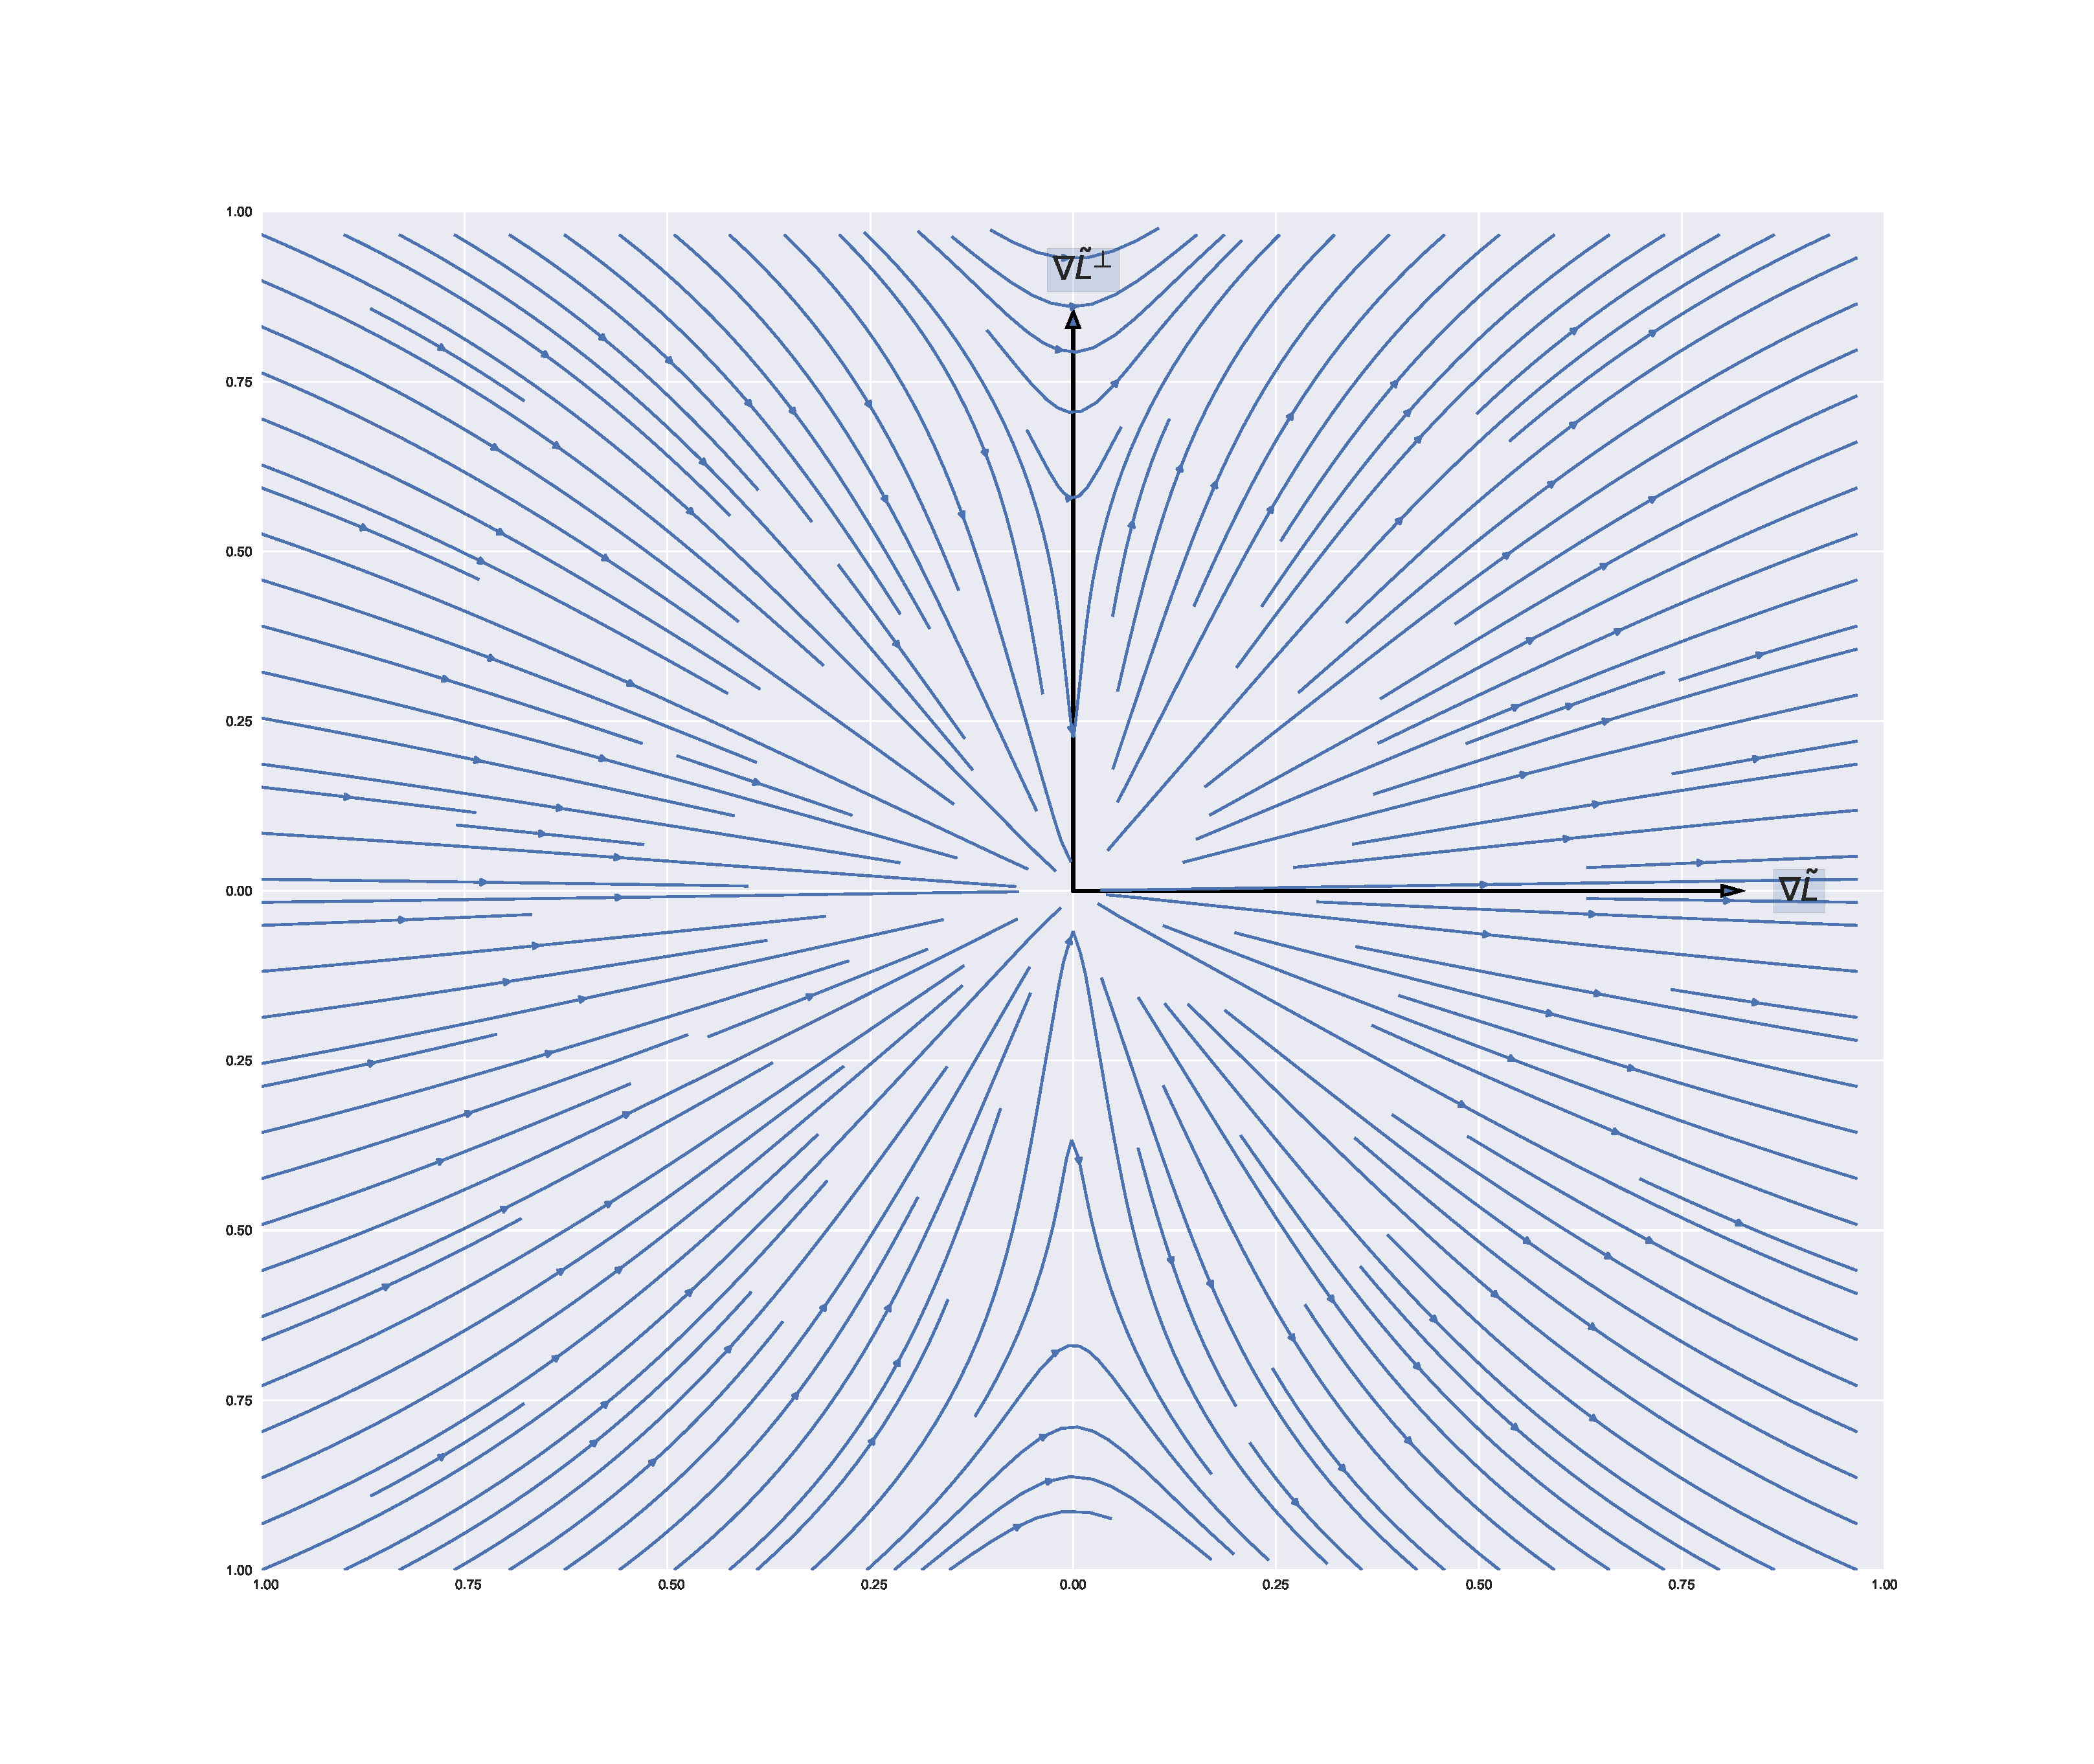
\includegraphics[width=\linewidth]{figures/dynamics_delta_-1.pdf}
    % \endminipage\hfill
    \minipage{0.33\textwidth}
    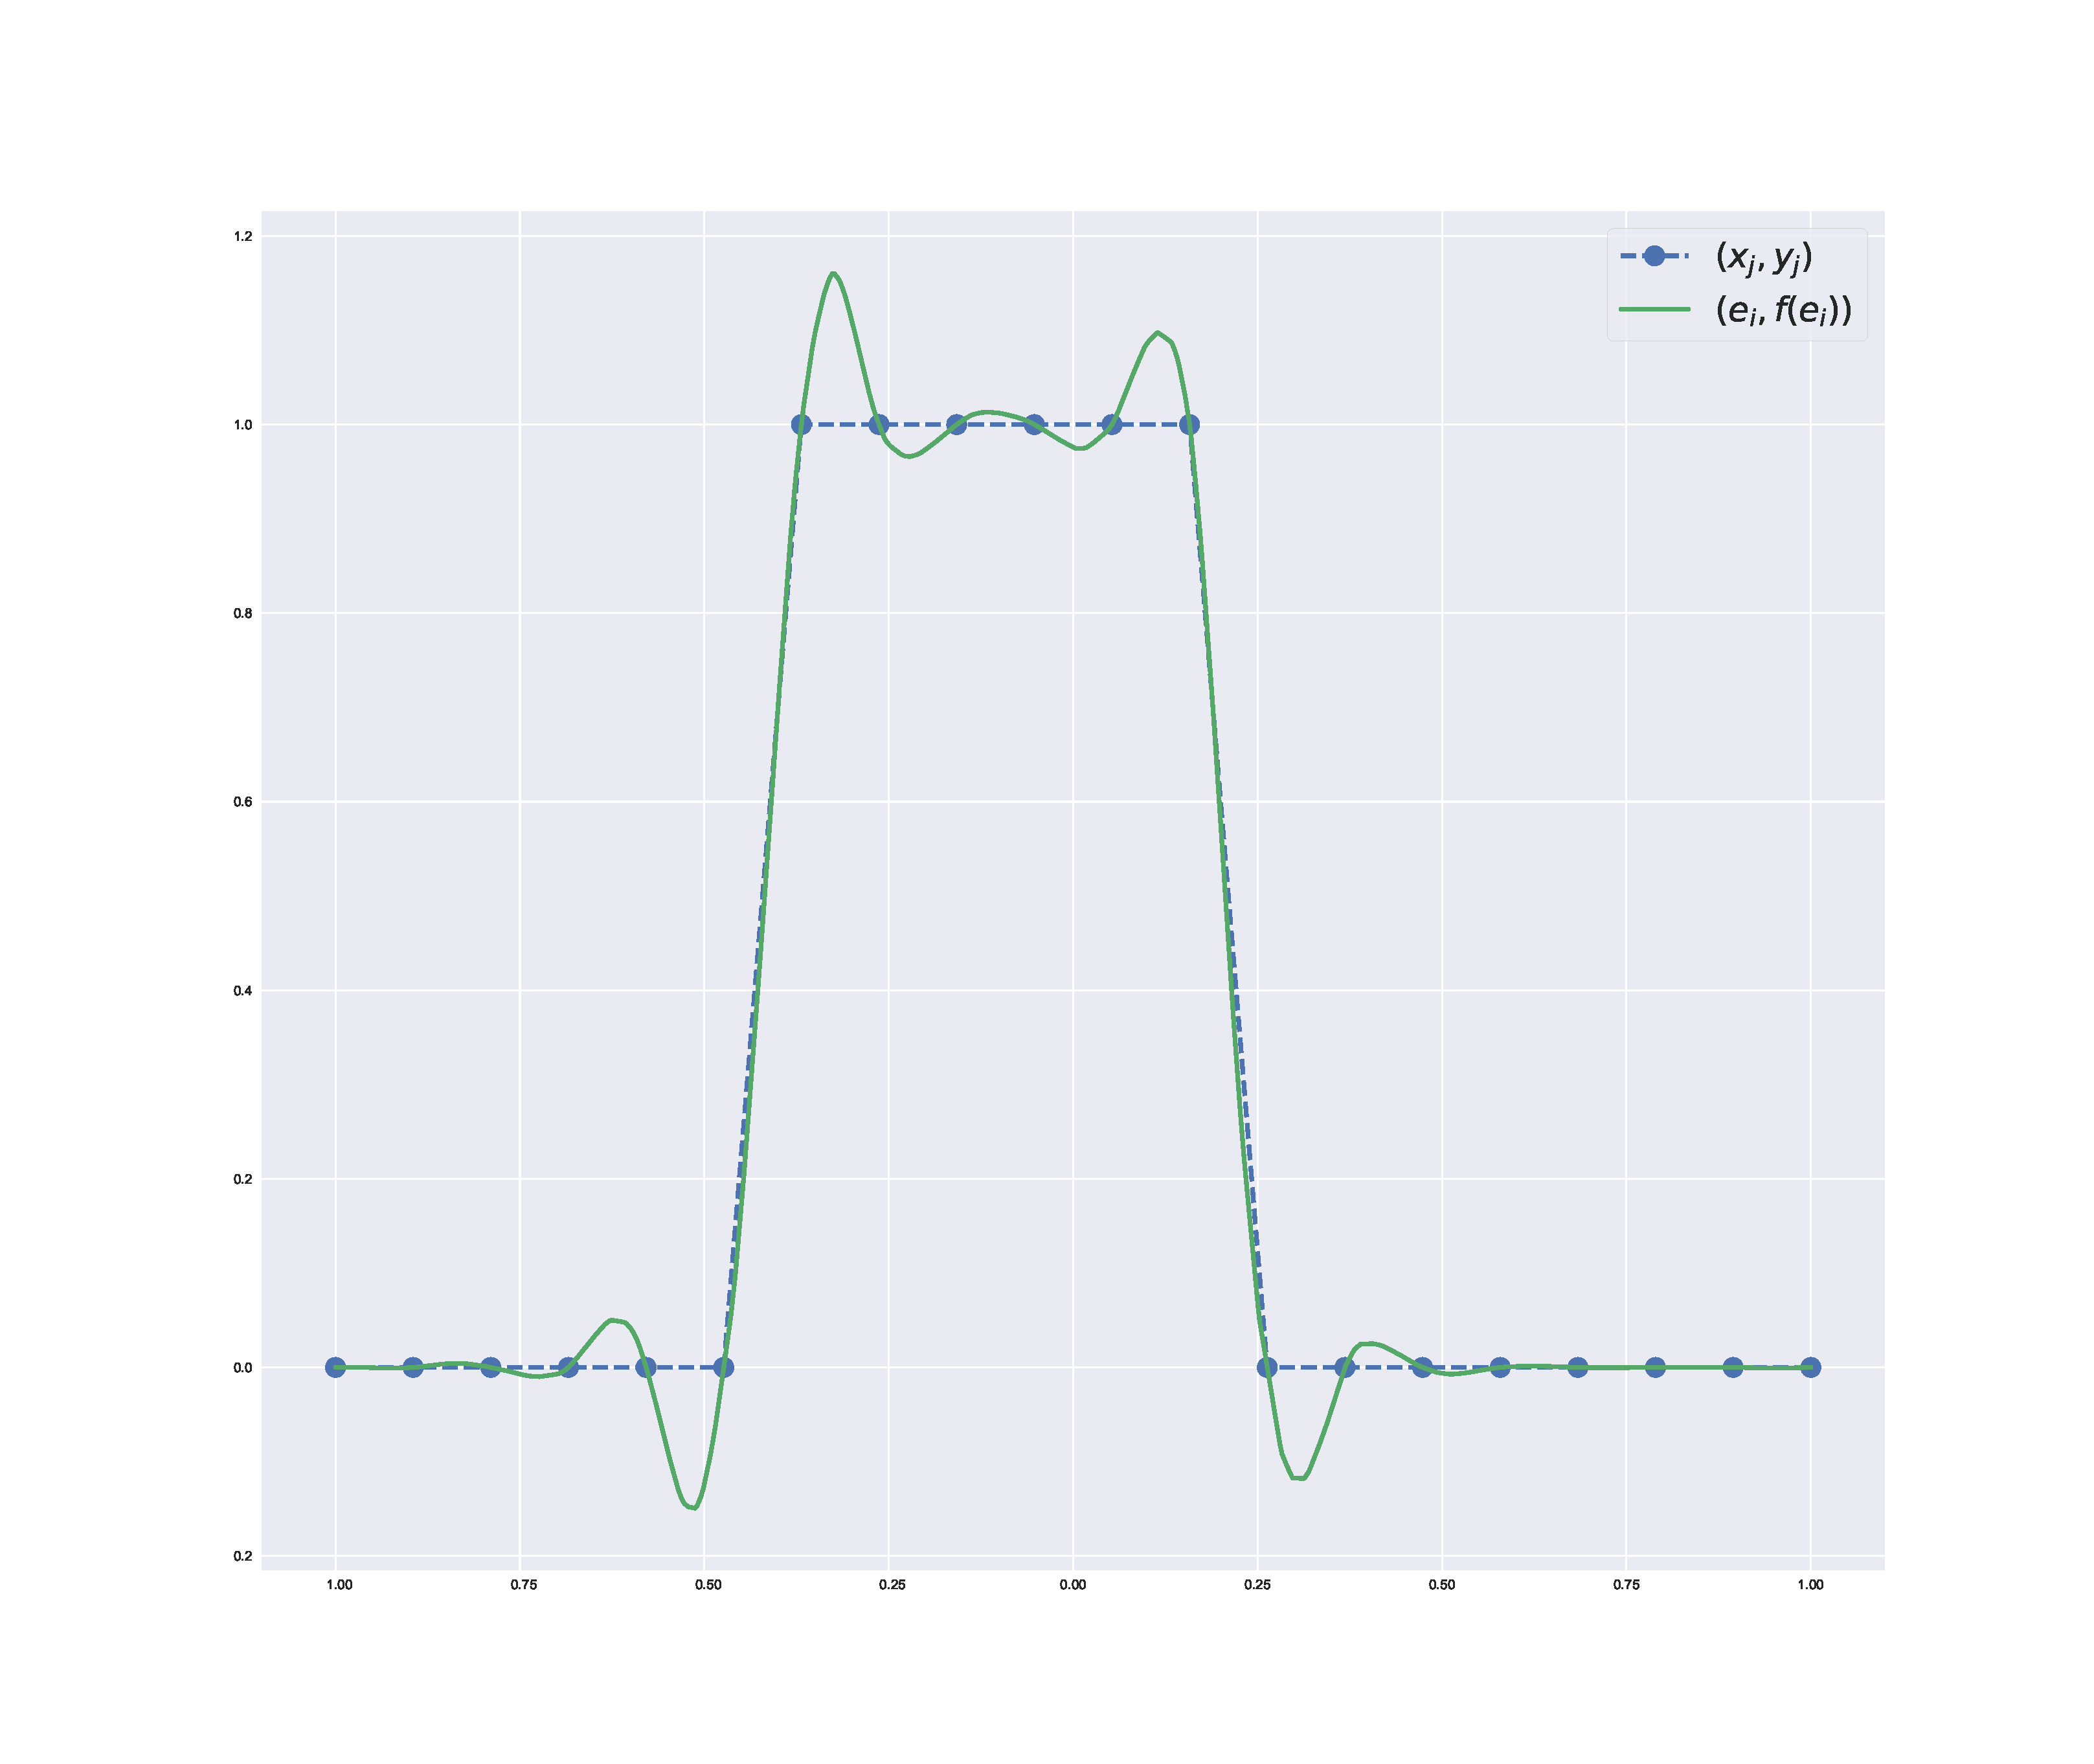
\includegraphics[width=\linewidth]{figures/same_init_different_func_square_1.pdf}
    \endminipage\hfill
    % \minipage{0.2\textwidth}
    % 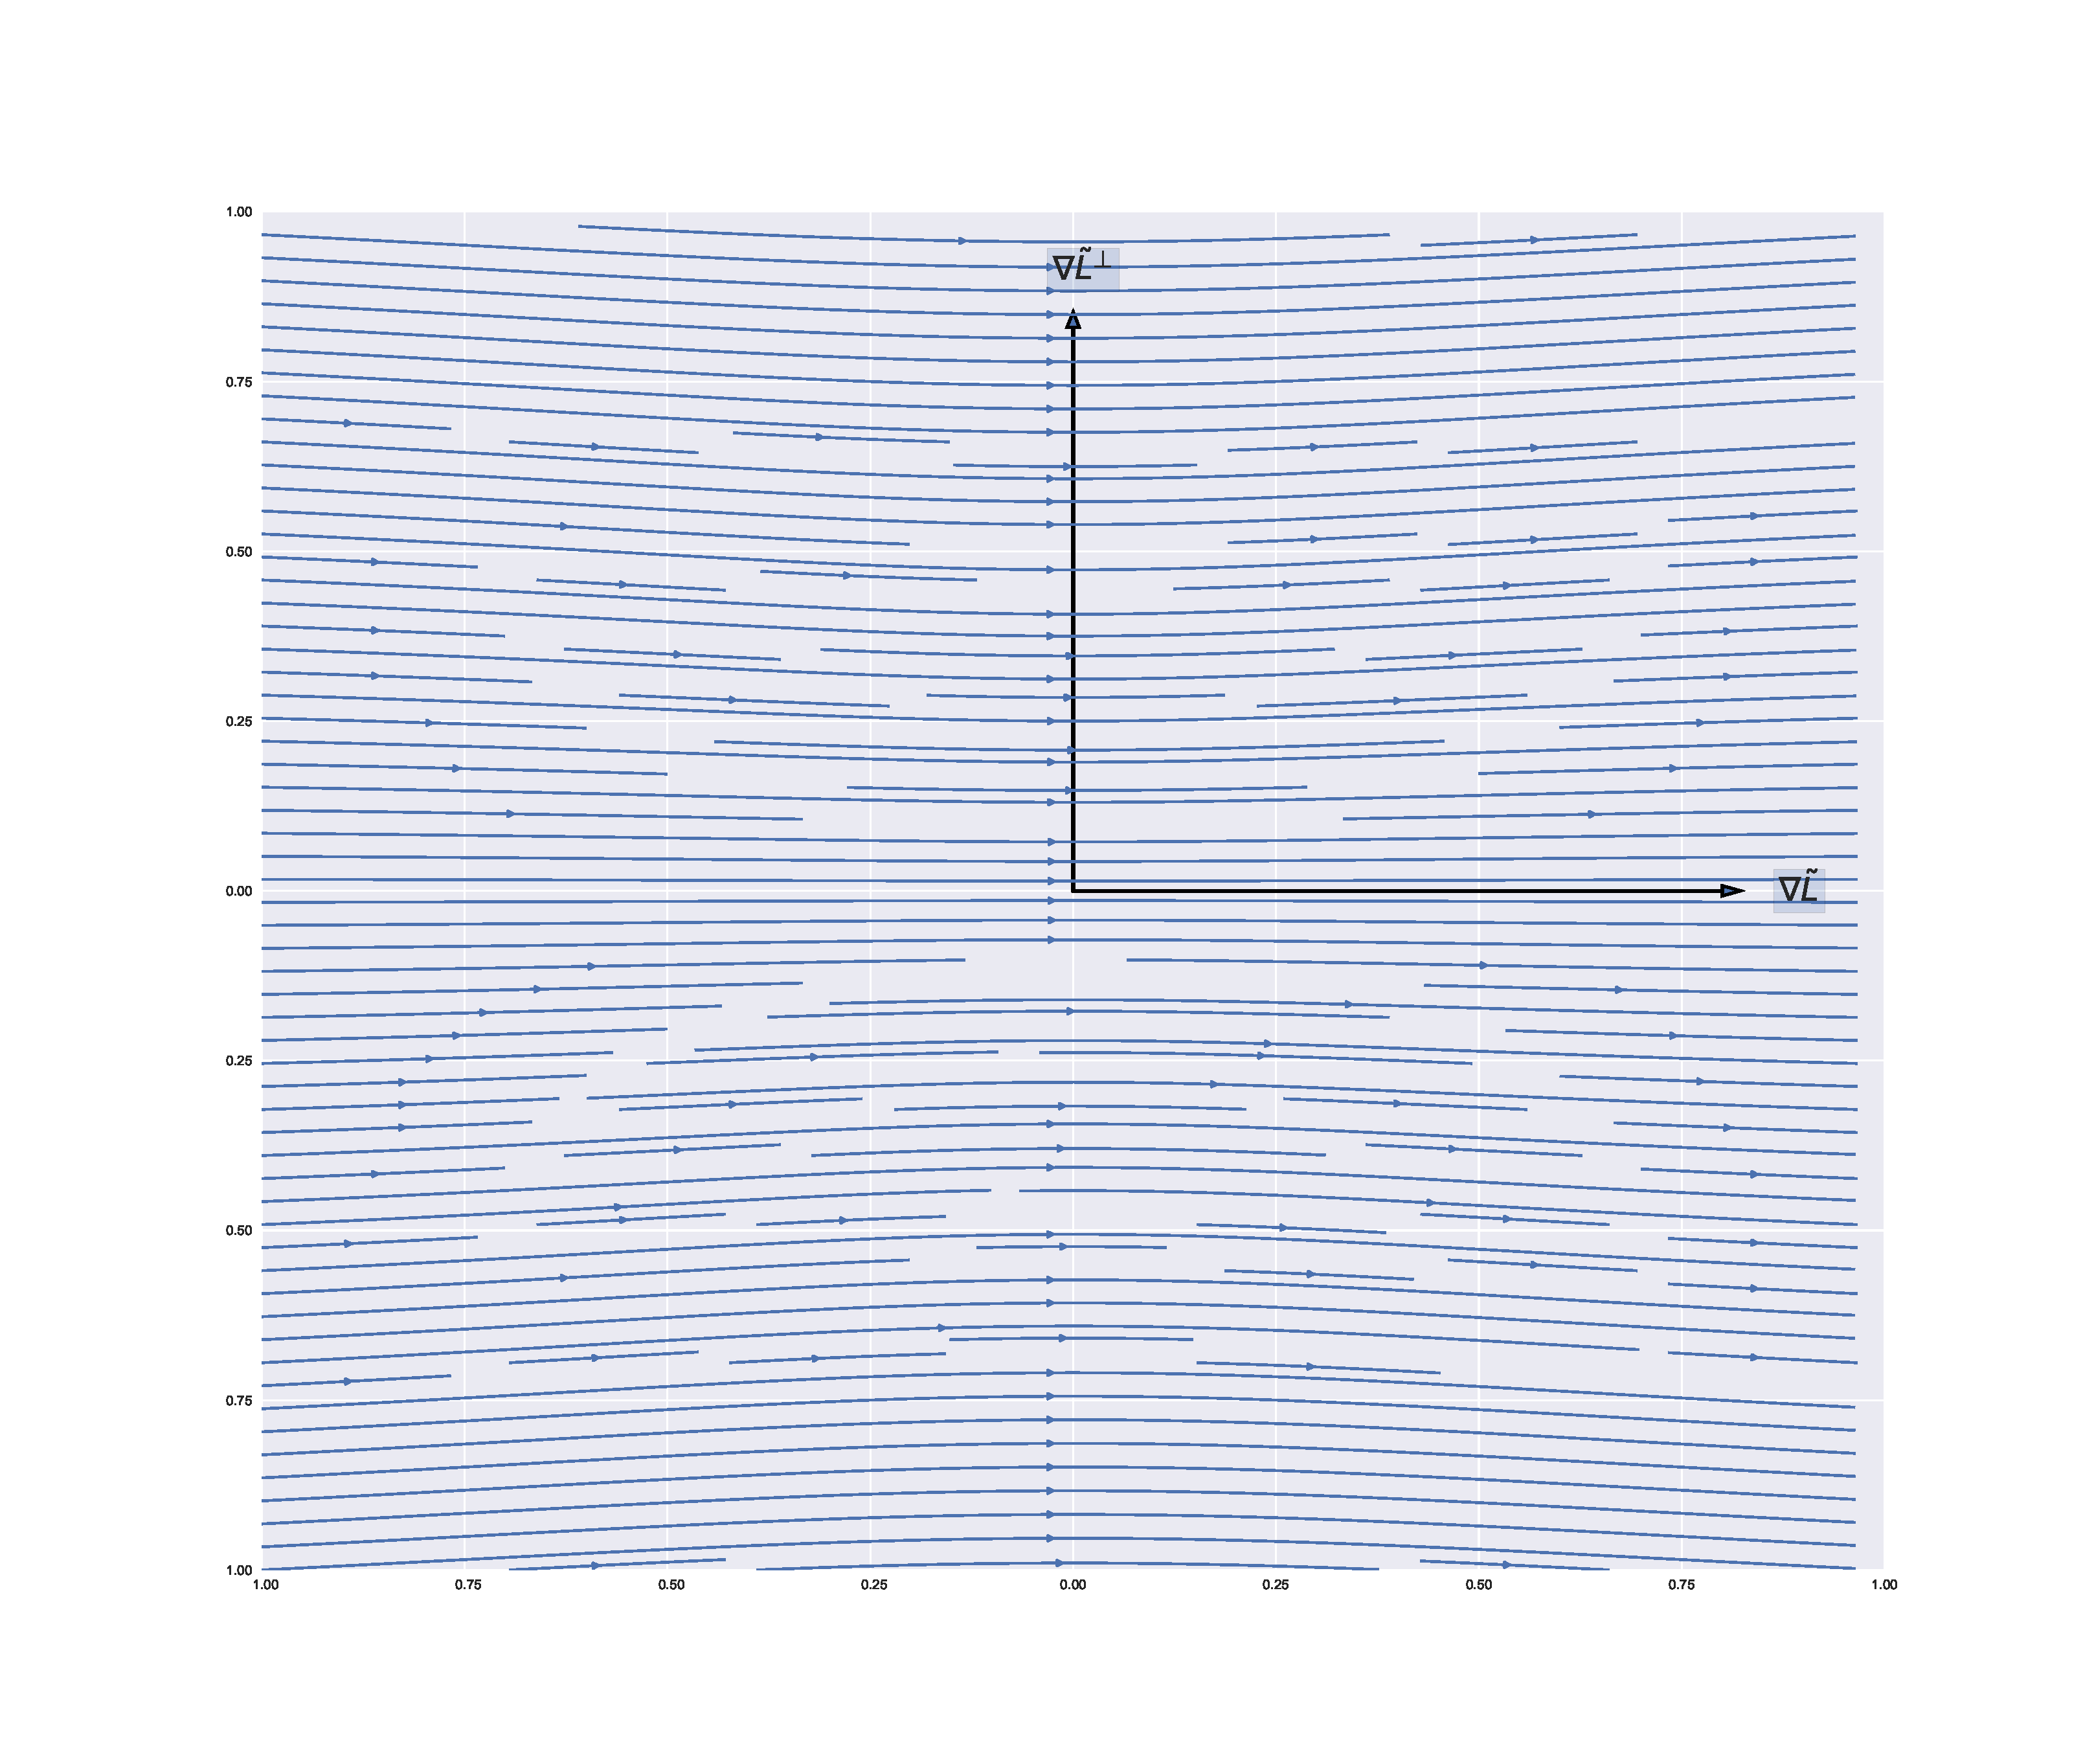
\includegraphics[width=\linewidth]{figures/dynamics_delta_1.pdf}
    % \endminipage\hfill
    \minipage{0.33\textwidth}
    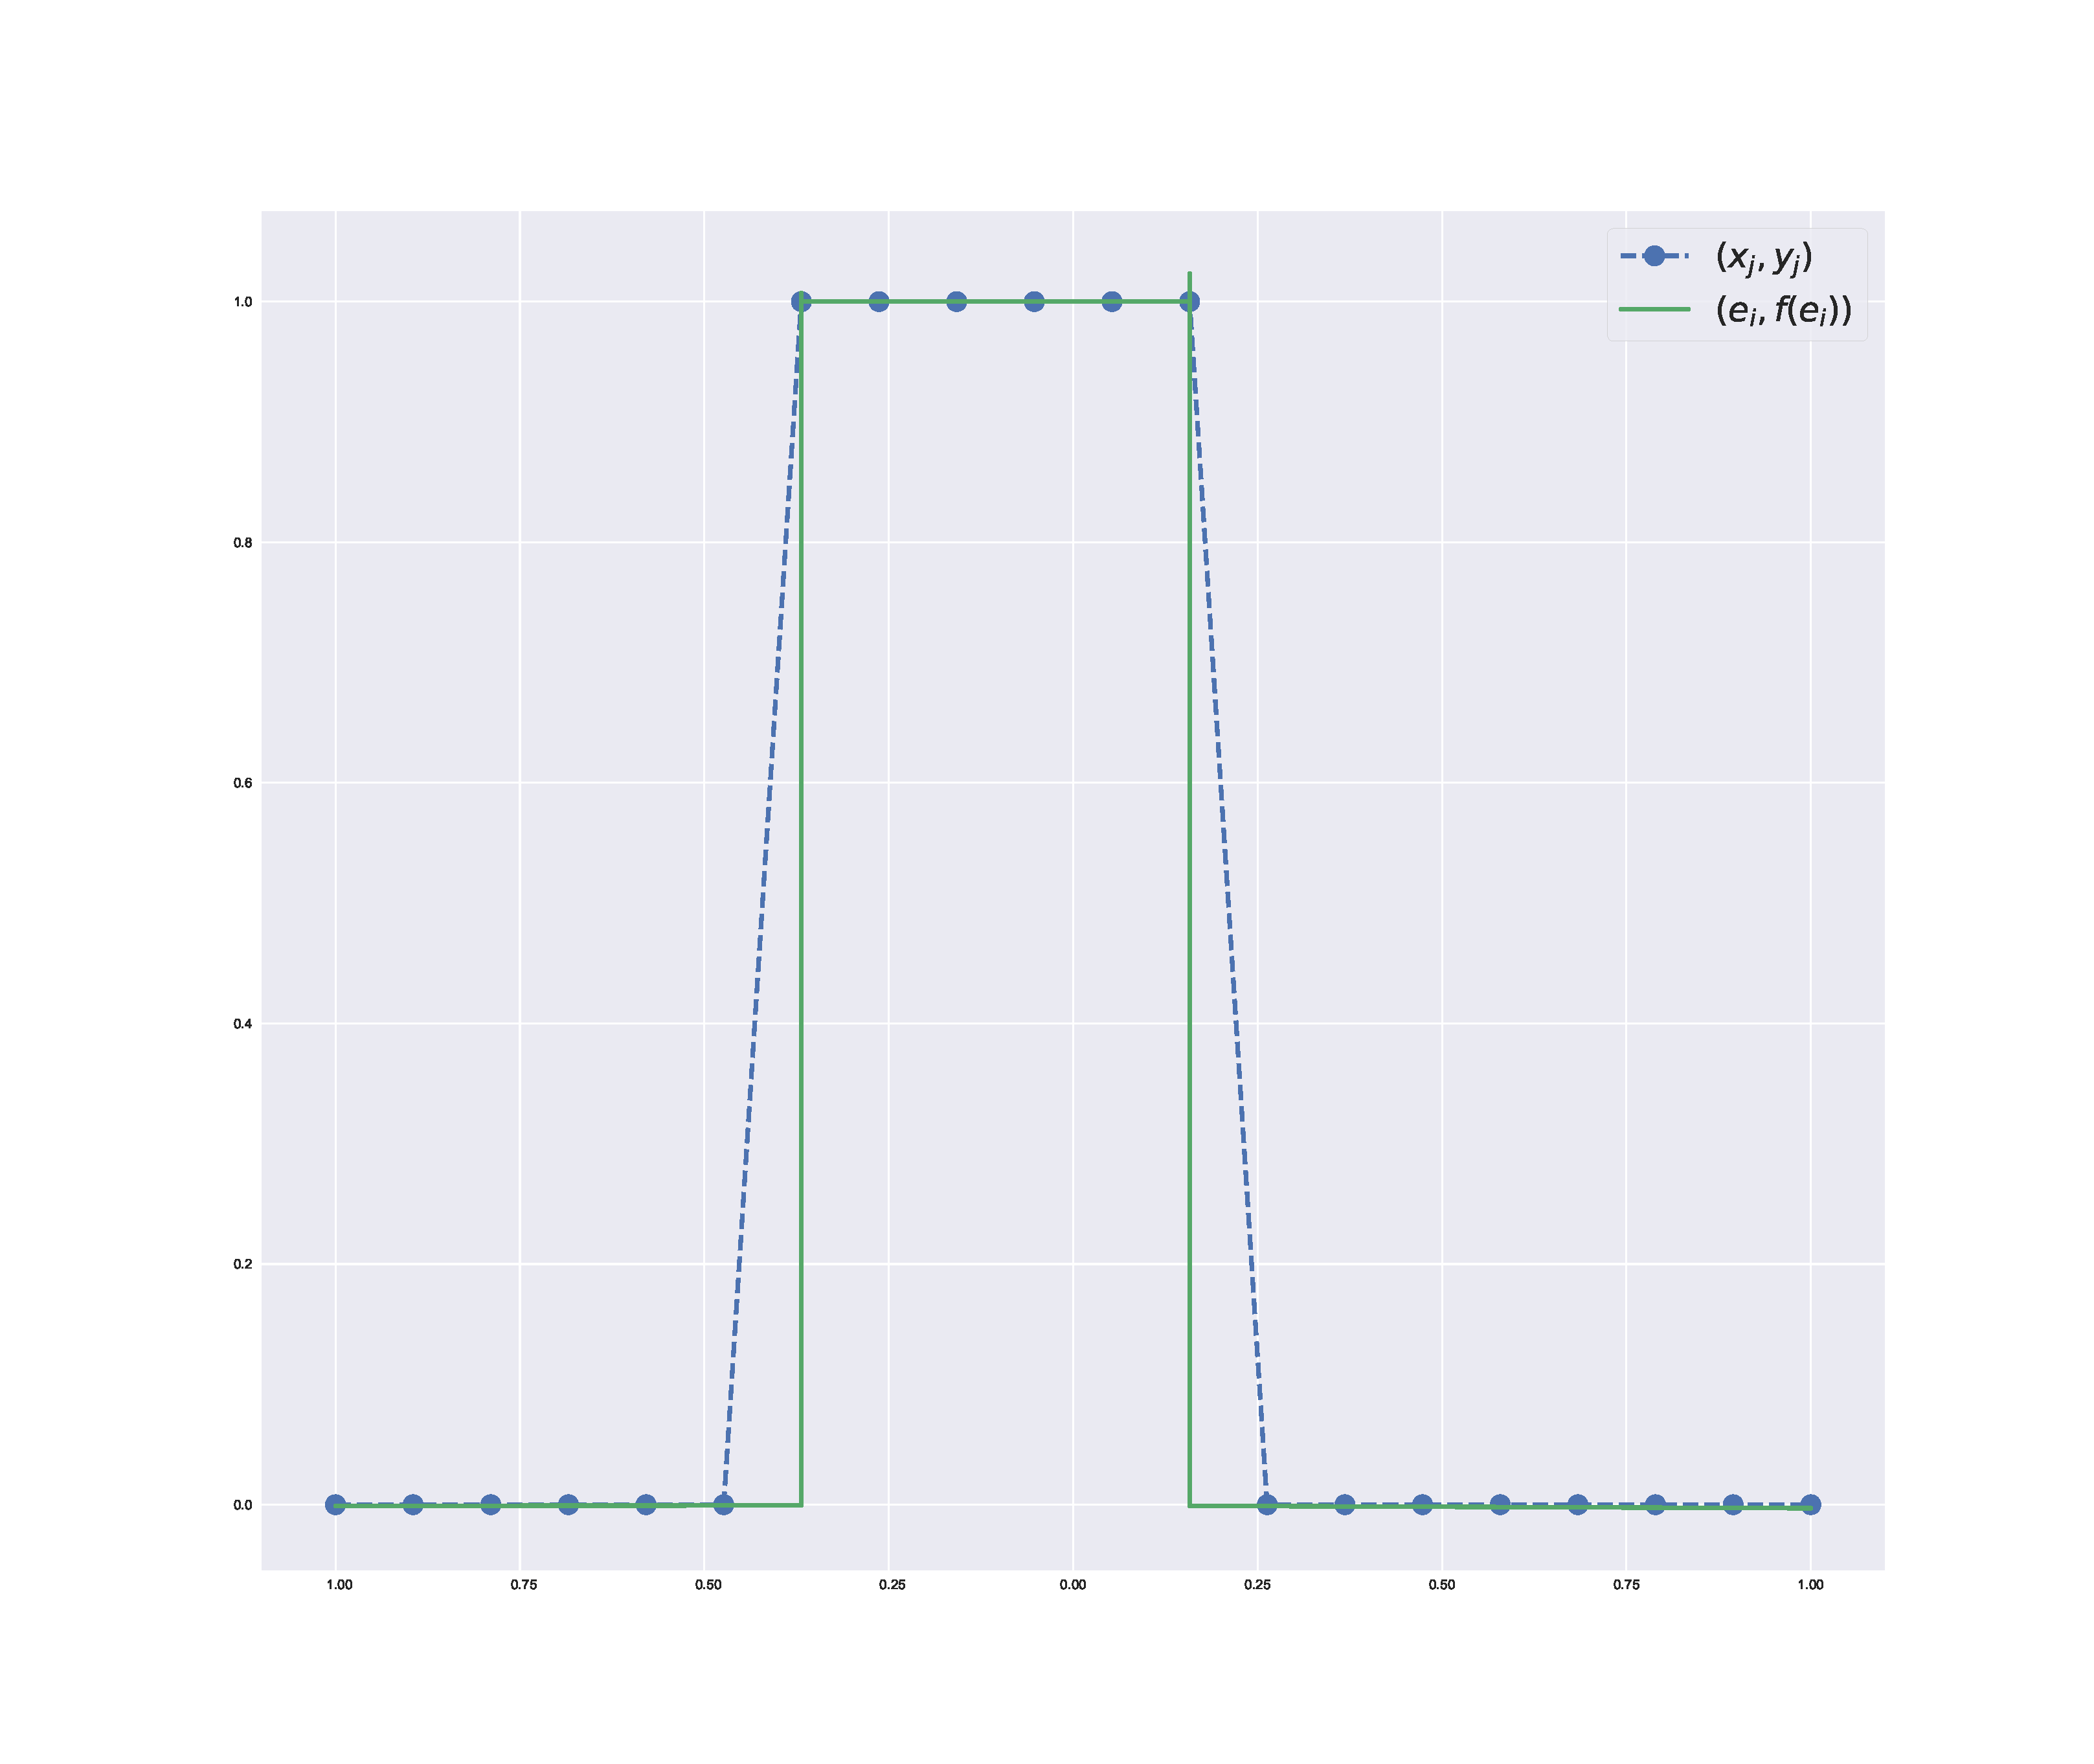
\includegraphics[width=\linewidth]{figures/same_init_different_func_square_1000.pdf}
    \endminipage
    
    \caption{The same initial function can yield very different results: the left image is the initial function for the two right ones. The initial parameters ($\bm a, \bm b, \bm c$) were the same as those in the middle image but scaled by a factor of 1000, 1000 and 0.001 respectively}
\end{figure}

\begin{figure}
    \centering
    \minipage{0.33\textwidth}
        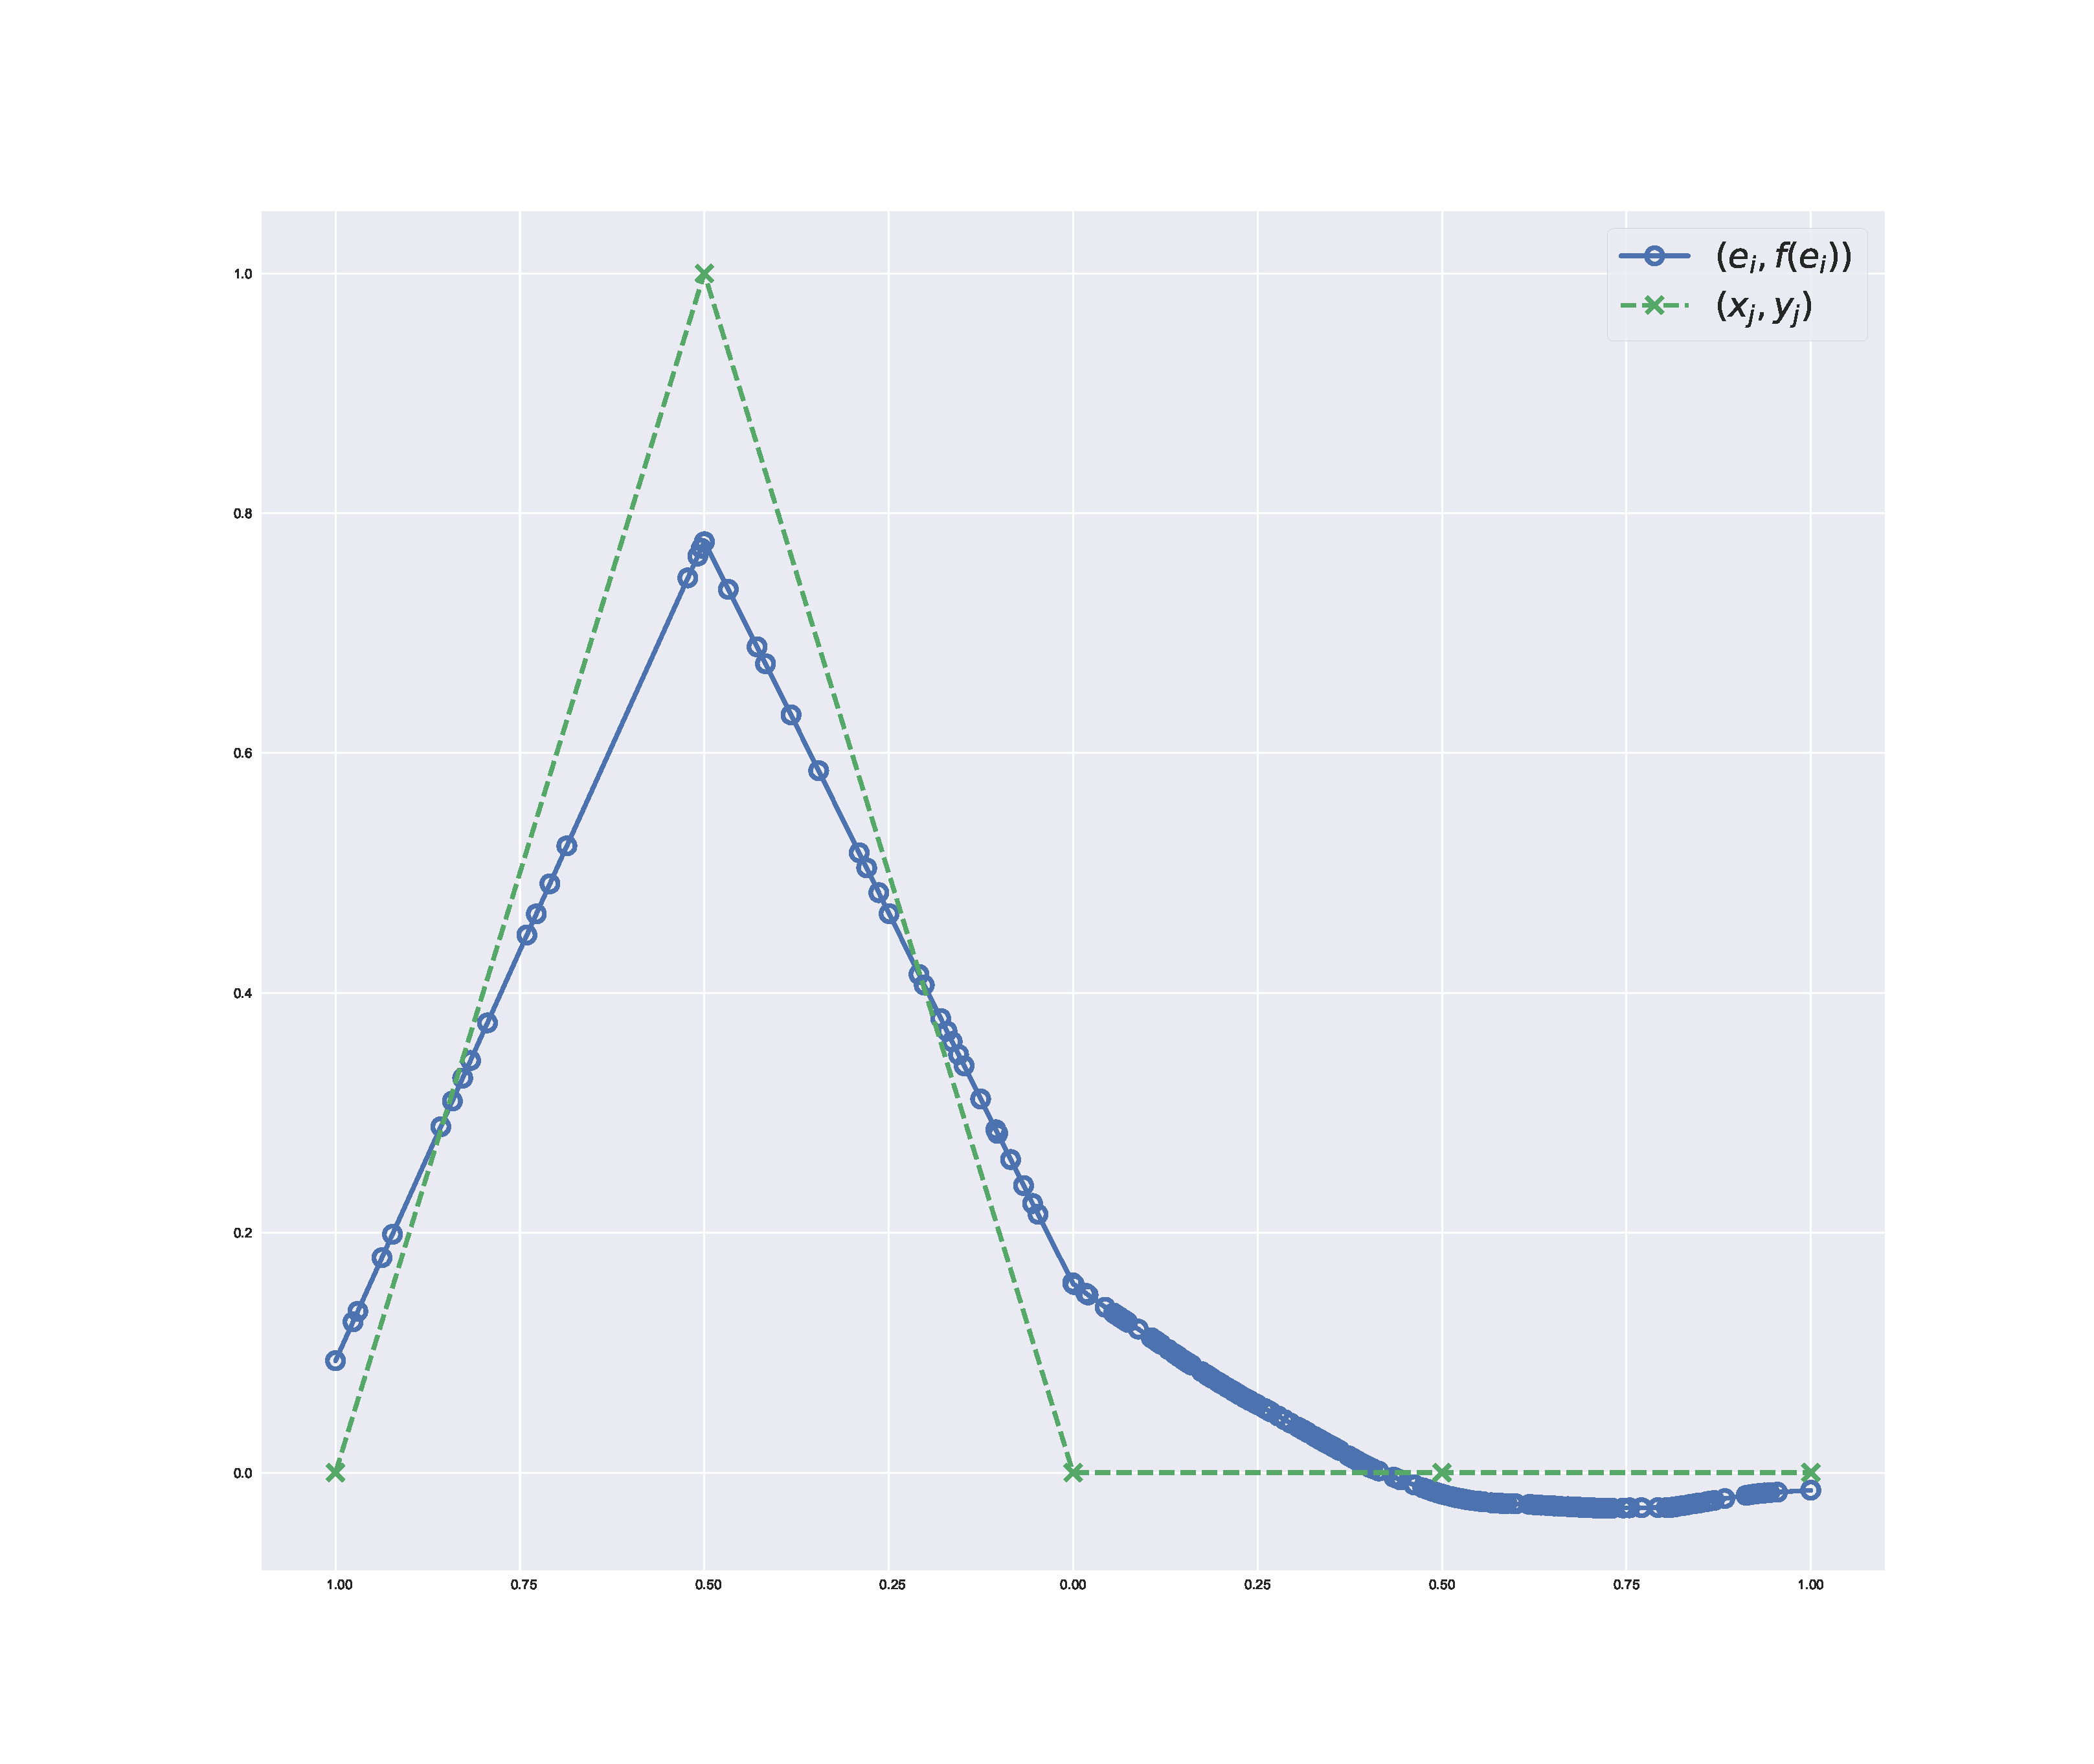
\includegraphics[width=\linewidth]{figures/reduced_gradient_recon.pdf}
    \endminipage
    \minipage{0.33\textwidth}
        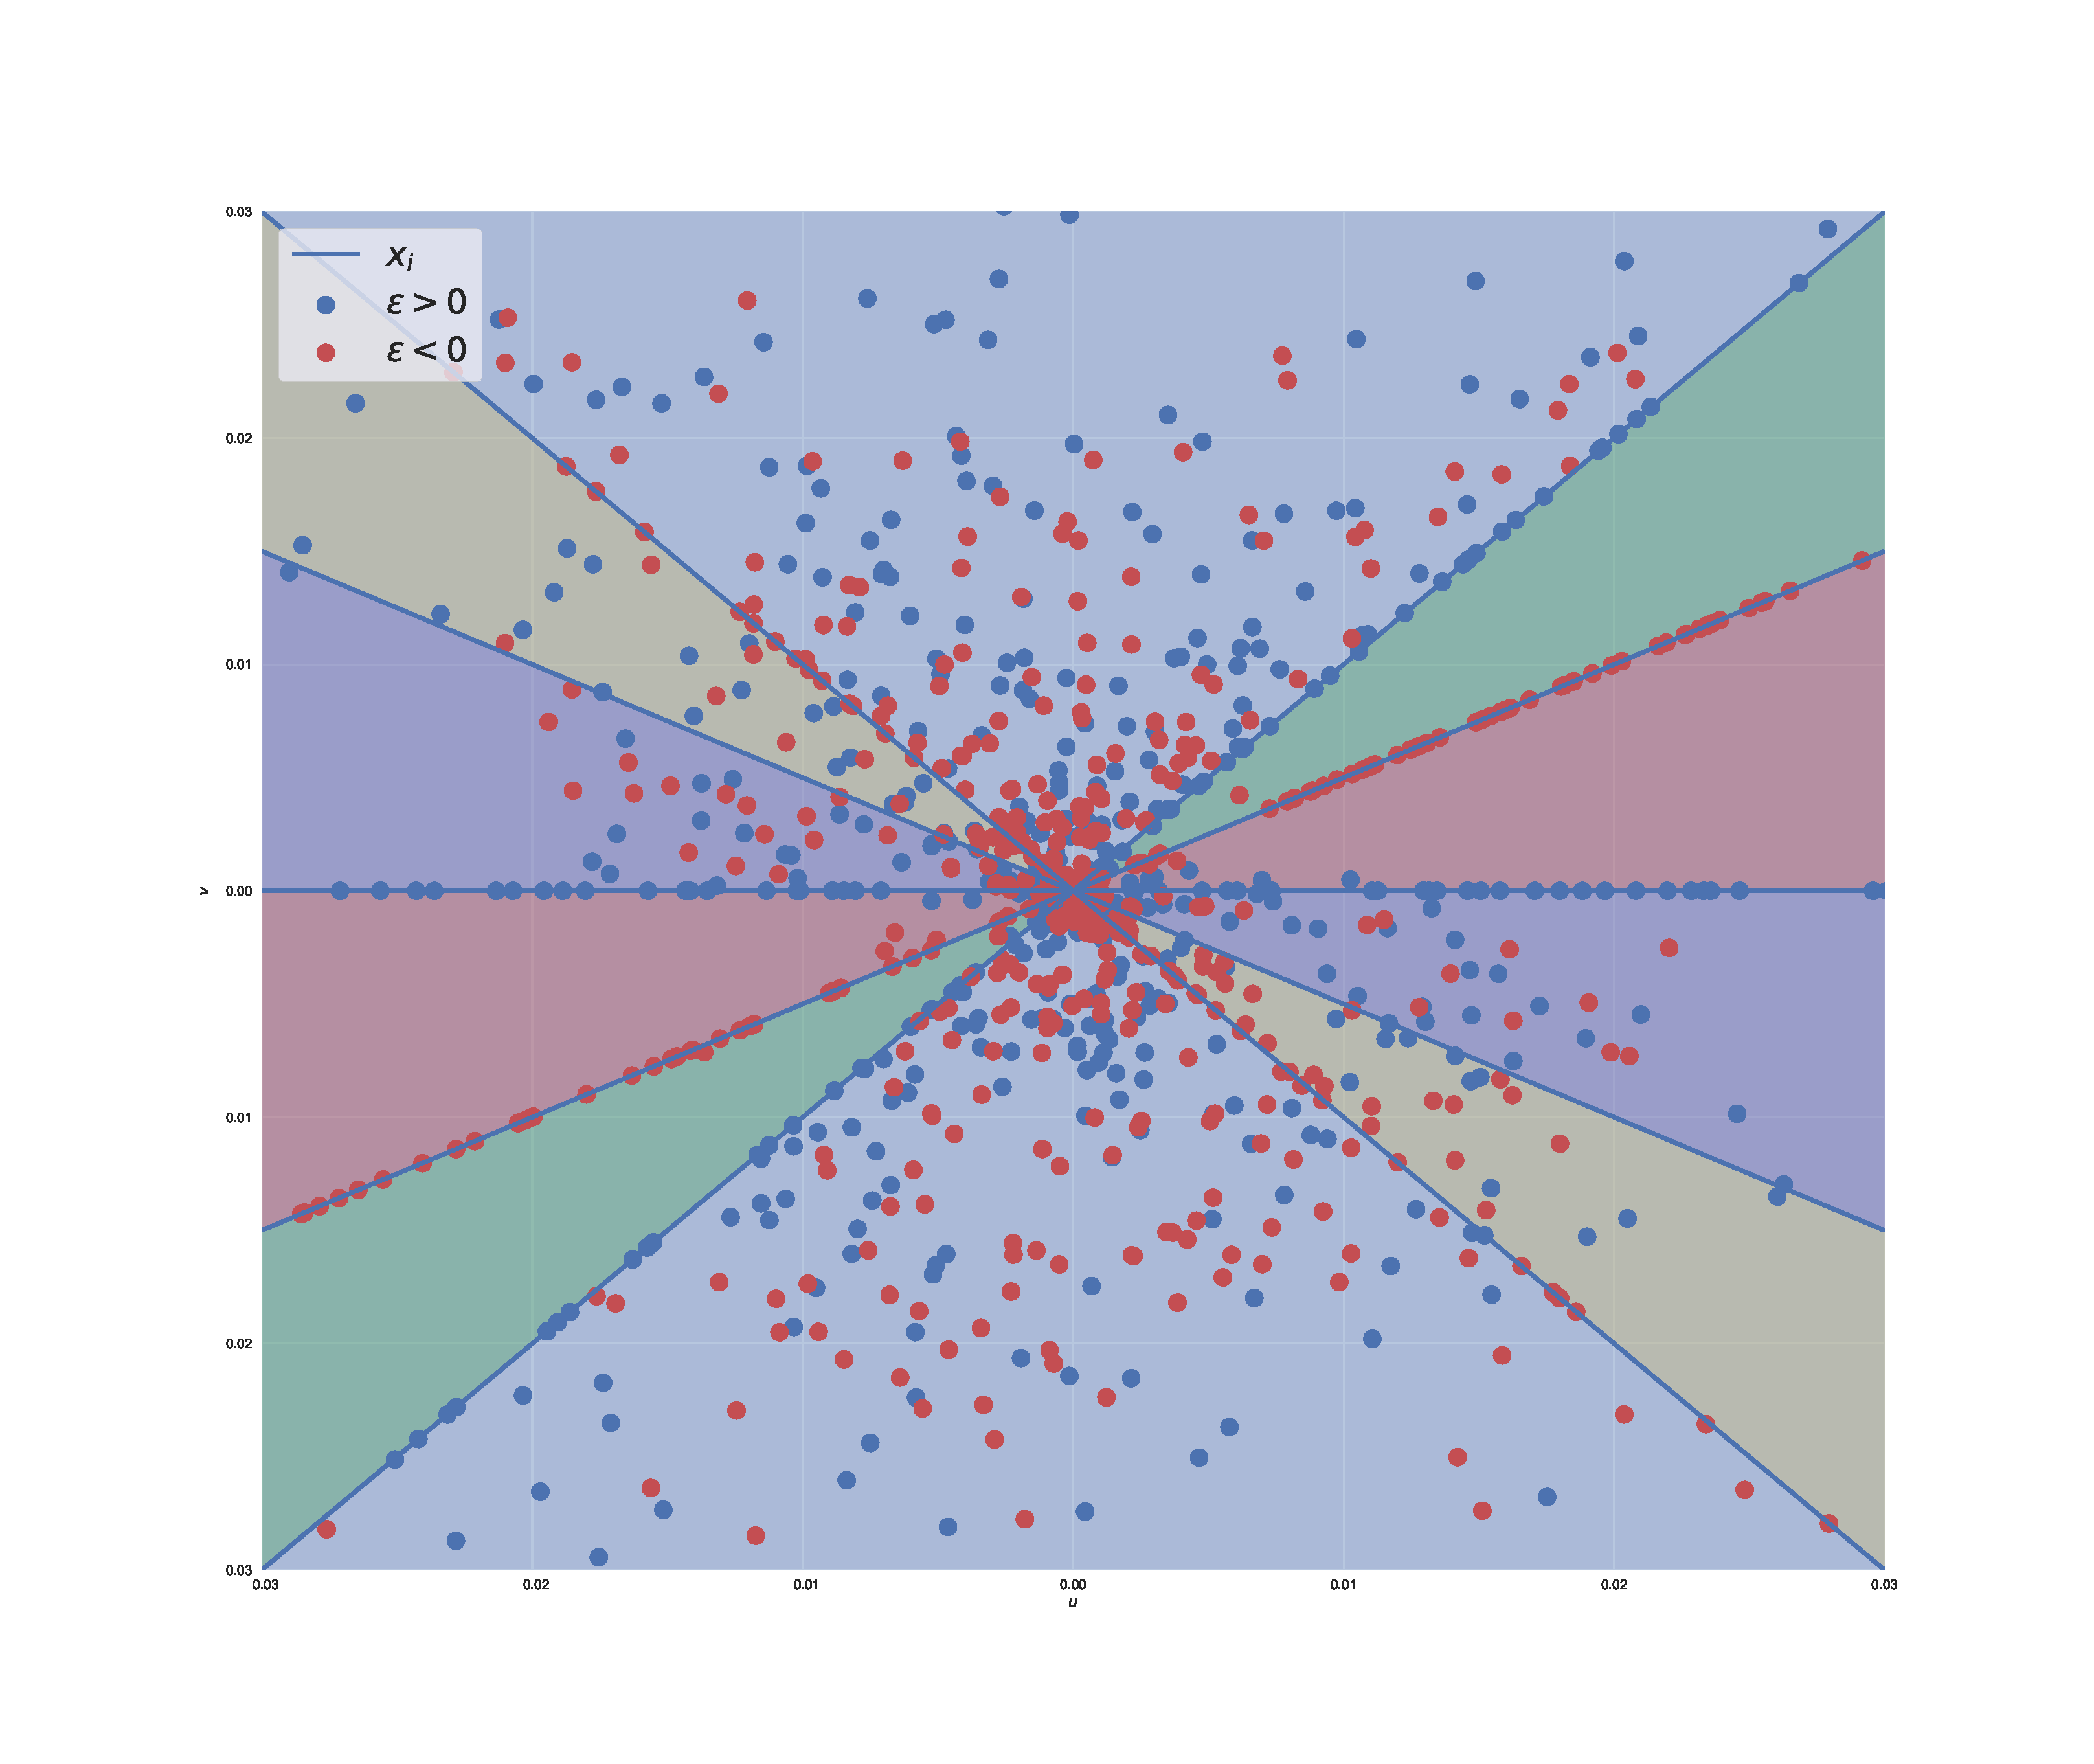
\includegraphics[width=\linewidth]{figures/reduced_gradient_phase.pdf}
    \endminipage
    \minipage{0.33\textwidth}
        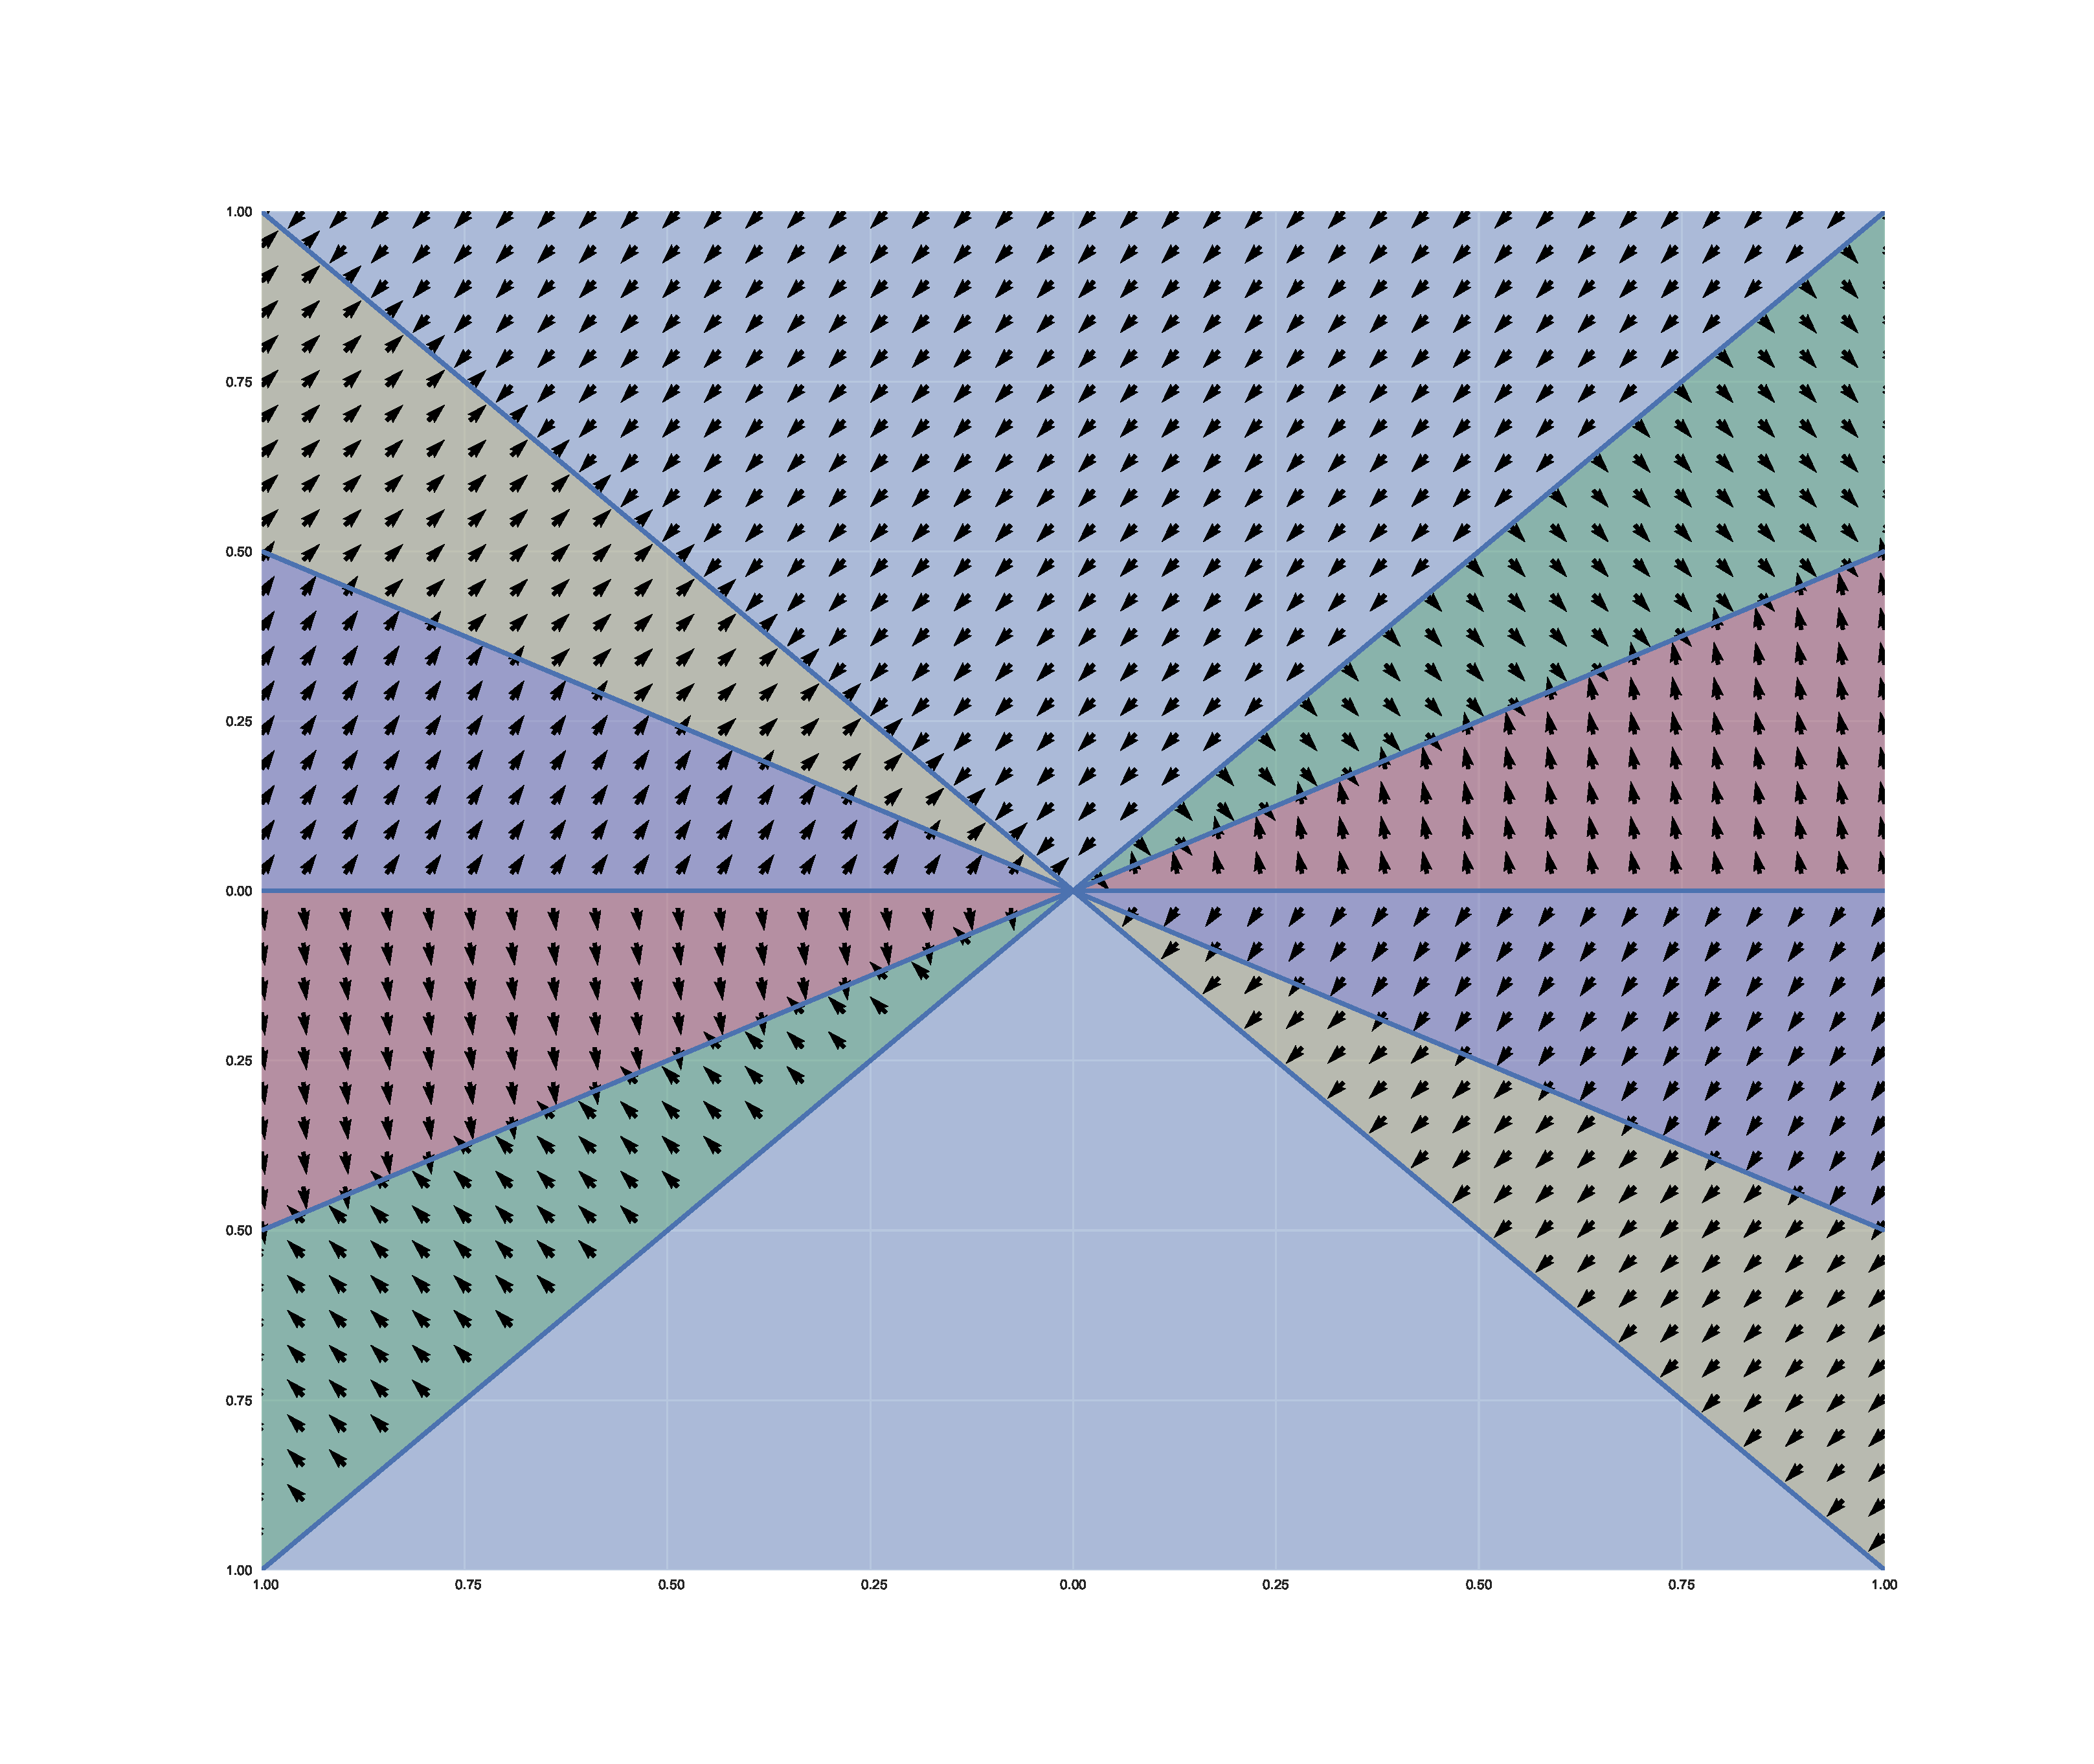
\includegraphics[width=\linewidth]{figures/reduced_gradient_vector_field.pdf}
    \endminipage\hfill
    \caption{The vector field of the gradient of the loss in reduced parameter space $\nabla \tilde{L}(\bm \xi)$. Note that the orientation of the arrow depends on the sign $\epsilon_i$ of a neuron. Thus, the gradient of the blue neurons are the arrows in the picture while the gradient of the red neurons point point in the opposite direction. We see in the middle image, that the neurons cluster on different samples depending on their sign.}
    \label{fig:reduced_grad}
\end{figure}
\section{Concluding Remarks}
\bibliography{main.bib}{}
\bibliographystyle{plain}
\newpage
\appendix

\section{Tangent Kernels and Gradient Flows}
Let $C: H \rightarrow \RR$ be a smooth function on a Hilbert space $H$ (for
our purposes, $H$ is either a space of functions or a Euclidean space
$\RR^m$). Inside $H$, we consider a subset $M_\Phi = \{\Phi (\theta) \, | \,
\theta \in \RR^{n}\}$ defined as the image a smooth map $\Phi: \RR^ {n} \rightarrow
H$. The map $\Phi$ is not necessarily injective, so that each $z \in M_\Phi$ may
have many different ``lifts'' $\theta$ for which $\Phi(\theta) = z$. We
are interested in solving the optimization problem

\begin{equation}
\min_{z \in M_\Phi} C[z]
\end{equation}

by using the parameterization provided by $\Phi$ and following the gradient
flow of $L(\theta) = C[\Phi(\theta)]$ in $\RR^n$. If $d \Phi(\theta):
\RR^{n} \rightarrow H$ is the differential of $\Phi$ at $\theta$, then for
every parameter $\theta$, we define a linear map $K(\theta): H
\rightarrow H$ as

\[
K(\theta) = d \Phi(\theta) \circ d \Phi(\theta)^*: H \rightarrow
H
\]

where $d \Phi(\theta)^*$ denotes the adjoint of $d \Phi(\theta)$. Since $K$ is self-adjoint, it also defines a positive semidefinite bilinear map $H
\times H \rightarrow \RR$. If $H = \RR^m$, then $K(\theta)$ can be identified
with $(m \times m)$-matrix $J_\Phi(\theta) J_\Phi^T(\theta)$ where $J_\Phi(\theta)$ is
the jacobian of $\Phi$. The operator $K$ is known as the~\emph{tangent kernel}
(although it may not be positive definite if $d\Phi$ is not surjective)~\cite{NTKJacot,chizat2018note}.

\begin{lemma} If $\theta(t)$ is an integral curve for the gradient vector
field $\nabla L$ in $\RR^{d_\theta}$, then corresponding curve $z(t) =
\Phi(\theta(t))$ in $H$ satisfies
\begin{equation}\label{eq:tangent_kernel}
\frac{d z}{dt}(t) = K(\theta(t)) \,\, \nabla C (\Phi(\theta(t))).
\end{equation}
where $\nabla C$ denotes the gradient of $C$ inside $H$.
\end{lemma}


From this lemma, we see that the tangent kernel can be viewed as a
``preconditioning map'' that modifies the gradient $\nabla C(z)$ in the space $H$ to correspond to the dynamics of gradient flow in the
parameter $\theta \in \RR^n$. On the other hand, we cannot in general
use~\eqref{eq:tangent_kernel} to ``forget'' the parameterization and describe
the dynamics purely inside $H$, given that $K(\theta)$ cannot be uniquely
associated with points $z$ in $H$, since it is generally not fixed
in the set of lifts $\{\theta \, | \, \Phi(\theta) = z\}$. 

\begin{remark} If the tangent kernel $K(\theta(t))$ hardly changes for a trajectory $\theta(t), t \ge 0$ then~\eqref{eq:tangent_kernel} can be approximated by
\begin{equation}
    \frac{d z}{dt}(t) = K(\theta(0)) \,\, \nabla C (\Phi(\theta(t))).
\end{equation}
The regime where this approximatation is valid is referred to as \emph{lazy training} in~\cite{chizat2018note}. It is shown in~\cite{NTKJacot} that if $\Phi$ represents the parameterization of a neural network, then lazy training occurs as the widths of the network go to infinity and for appropriate initializations (using a normalization by $1/\sqrt{m_\ell}$ where $m_\ell$ is the width of a layer). \note{If we use this, explain more?}
\end{remark}

note{Qualitative description of ODE.}



We now discuss how the matrix $K(\xi)$ applied to the vector field $\nabla \tilde{L}$ yields different types of neuron trajectories.
% $(\beta a^2+ \beta b^2 + \alpha c^2, (a,b))$ and $(\alpha c^2, (-b,a))$, which correspond to radial and tangential components of $(u, v)$. From this we deduce that

\begin{lemma}\label{le:pw_continuous}
The gradient in the reduced parameter space, $\nabla \tilde{L}$ is piecewise linear with discontinuities occuring precisely along radial lines corresponding to samples, i.e. $u = -x_i v$ for $i = 1, \ldots s$.
\end{lemma}

\begin{proof}
\note{Francis: Clean up the proof I have on paper and transcribe it. We will put this in the appendix since the lemma is sort of intuitive anyway.}
\end{proof}



When $\delta \ll -\|\xi\|$, then $c^2 \ll a^2 + b^2$, and the trajectory of neurons in the $(u, v)$-plane is mostly radial away or towards the origin (\todo{Figure \ref{fig:todo}}).

In the extreme case, where $\alpha c^2 = 0$, then the inner layer parameters, $a$, and $b$ remain stationary. Thus, the radial regime is equivalent to fixing the alternant matrix $M(a, b)$ and optimizing over the parameters, $c$. We can then view the function $f(x)$ as as a linear combination of basis functions $[a_i x + b_i]_+$ with coefficients $c_i$. We note that in radial training, the boundaries of linear pieces in the domain do not change. 

To study the dynamics of radial training, we can rewrite the function $f$ in terms of a fixed kernel $K(x, y)$ which depends only on the parameters $a$ and $b$. As shown in \cite{NTKJacot}, the finite kernel associated with a neural network converges as the number of weights grows large. Since our finite kernel $K$ is fixed in radial training (due to $a$ and $b$ being stationary), we can view the finite kernel as an approximation of the infinite one. By analyzing the properties of the infinite kernel, we can understand the behavior of the finite one.



\paragraph{Dynamics of Gradient Flow in Radial Training}
We now consider the dynamics of gradient flow in the radial regime.  If we minimize the loss, $\frac{1}{2}||Mc - y||^2$ with gradietn flow, we have that $c(t)$ follows the ODE \note{(This derivation is similar to \cite{NTKJacot})}

\begin{equation}
\begin{aligned}
    \partial_t c(t) &= -\nabla_c \frac{1}{2} ||M c(t) - y||^2\\
                    &= -(M^T M c(t) - M^T y)
\end{aligned}
\end{equation}

and $f(x, t) = Mc(t)$ evolves according to

\begin{equation}
\begin{aligned}
\partial_t f(x, t) &= M \partial_t c(t)\\
                   &= M M^T y - M M^T Mc(t)\\
                   &= Ky - K f(x, t)
\end{aligned}
\end{equation}

which is a separable ODE with solutions of the form

\begin{equation}
    f(x, t) \propto y + \exp{(-K)} \mathds{1}t
\end{equation}

Decomposing $K$ into its eigenbasis we can write the evolution of the residual as

\begin{equation}
    r(t) = f(t) - y \propto \sum_{j=1}^s \exp{(-t\lambda_i \mathbf{e_i})}
\end{equation}

where $(\lambda_i, \mathbf{e_i})$ are $i^\text{th}$ eigenvalue/eigenvector pair of $K$. In the overparameterized case, this gradient flow will minimize the least squares loss \eqref{eq:lsq_overparameterized} for initializations of $c$ with small norm. Observe that the eigenfunctions of $K$ with large eigenvalues decay first which acts as a regularizer when stopping gradient descent early as these eigenfunctions typically correspond to lower frequency features of the function being fit. \note{(An interesting practical fact is that we can perturb the kernel by $\epsilon I$ and solve the linear system to get smoother solutions)}


Observe that $(M M^T)_{ij}$ can be written as the inner product 

\begin{equation}\label{eq:lsq_kernel}
(M M^T)_{ij} = \langle [a x_i + b]_+, [a x_j + b]_+ \rangle = K(x_i, x_j)
\end{equation}

where $K(x_i, x_j)$ is a positive definite kernel if $rank(M) = s$. Denoting the matrix, $M M^T$ as $K$ and observing that $f(x_i) = (Mc)_i$, we can write

\begin{equation}
\begin{aligned}
Mc &= f(x)\\
   &= M M^T (M M^T)^{-1} y\\
   & = K K^{-1}y\\
   & = Kv
\end{aligned}
\end{equation}



Functions of the form~\eqref{eq:ReLU1D} are \emph{continuous piecewise linear} (CPL). If $f$ is CPL, the extreme points of the intervals where $f$ is linear are called the \emph{knots}. For 1D functions, knots are a convenient way of visualizing the neurons of a function. Figure~\ref{fig:knots} shows an example of such a function and its knots. Assuming that $a_i \neq 0$ for all $i$, the knots are given by:

\begin{equation}\label{eq:nodes}
e_1 = -\frac{b_1}{a_1}, \ldots, e_m = -\frac{b_m}{a_m}.
\end{equation}

Indeed, these are the points where the operand inside a ReLU activation changes sign. Perhaps counterintuitively, the function space $\mathcal F$ is a strict subset of the space of CPL maps with $m$ knots, but it contains the set of CPL maps with $m-1$ knots \note{Lemma in sup mat?}.

We denote the least squares loss in \eqref{eq:leastsquares} by
\begin{equation}\label{eq:nnloss}
    L(\theta) = \frac{1}{2}\sum_{j=1}^s ||r_j(\theta)||^2 \qquad r_j(\theta) = f_\theta(x_j) - y_j
\end{equation}

where $r_j(\theta)$ is the \emph{residual} at the sample $x_j$. In our setting, it is convenient to rewrite the evaluation of $f_\theta$ at the samples $x = (x_i)_{i=1}^s$ as the matrix product:

\begin{equation}
    f(x) = (M_x(a, b) c),
\end{equation}

where $M_x(a, b)$ is the \emph{alternant matrix} defined as

\begin{equation}\label{eq:alternant_matrix}
\begin{aligned}
M_x(a, b) = 
\begin{bmatrix} 
    [a_1 x_1 + b_1\ge 0]_+ & \ldots & [a_m x_1 + b_m\ge 0]_+\\
    \vdots                 &        & \vdots\\
    [a_1 x_s + b_1\ge 0]_+ & \ldots & [a_m x_s + b_m\ge 0]_+\\
\end{bmatrix} \in \RR^{s \times m}.
\end{aligned}
\end{equation}

It is also convenient to define the \emph{activation matrix} whose entries are 1 or 0 depending on whether the operand of ReLU for a given neuron is active at a given sample
\begin{equation}\label{eq:activation_matrix}
\tau_x(a, b) = 
\begin{bmatrix} 
\mathds{1}[a_1 x_1 + b_1\ge 0] & \ldots & \mathds 1[a_m x_1 + b_m\ge 0]\\
\vdots                         &        & \vdots\\
\mathds{1}[a_1 x_s + b_1\ge 0] & \ldots & \mathds 1[a_m x_s + b_m\ge 0]\\
\end{bmatrix} \in \{0,1\}^{s \times m}.
\end{equation}

We say that the network, $f_\theta$ is \emph{overparameterized} if there are more neurons than samples (i.e. $m > s$). We now show that under mild conditions in the overparameterized case, we can always achieve zero-loss.

\begin{proposition} If $m > s$ and $\theta^*=(a^*, b^*, c^*)$ is a critical
point for $L(\theta)$ such that $M_x(a^*, b^*) \in \RR^{m \times s}$ has maximal rank $s$, then
necessarily $L_S(\theta^*) = 0$ (\ie, $f_{\theta^*}$ interpolates the
samples).
\end{proposition}

\begin{proof} 
    We consider the evaluation mapping
    \begin{equation}
    \Psi_x: \RR^{d_\theta} \rightarrow \RR^{s}, \qquad \theta \mapsto (f_\theta(x_1),\ldots,f_\theta(x_s)).
    \end{equation}
    If $m > s$ and $M_x(a^*,b^*)$ has full rank, then the evaluation map $\Psi_S$ is a
    \emph{submersion} at $\theta^*$, that is, the Jacobian $J \Psi_x
    (\theta^*)$ of $\Psi_x$ has full rank. Indeed, the last $m+1$ columns of $J\Psi_x(\theta^*)$ are exactly $M_x(a^*,b^*)$:
    \begin{equation} J\Psi_x(\theta^*) = \begin{bmatrix} \frac{\partial
    \Psi_x}{\partial \alpha}(\theta^*) & \frac{\partial \Psi_x}{\partial
    c}(\theta^*)\end{bmatrix} =
    \begin{bmatrix} \frac{\partial \Psi_x}{\partial \alpha}(\theta^*) &
    M_x(a^*,b^*) \end{bmatrix} \in \RR^{s \times d_{\theta}}
    \end{equation}
    Finally, the fact that $J \Psi_S(\theta^*)$ has full rank implies that $f_{\theta^*}$
    interpolates $S$ since
    \begin{equation}
    \nabla L(\theta^*) = (\Psi_x(\theta^*) - y)^T \cdot J \Psi_x(\theta^*)
    = 0 \Rightarrow \Psi_x(\theta^*) = y.\end{equation}
\end{proof}
This proposition shows that either a critical point $\theta^*$ for $L$
corresponds to and interpolant function $f_{\theta^*}$ (a global minimum for
$L$), or the corresponding alternant matrix $M_x(a^*,b^*)$ must have
non-maximal rank. If $m \gg s$, we expect $M_x (a,b)$ to have full rank for almost all choices of $\theta$.

\begin{proposition} Let $e_1 \le \ldots \le e_m$ be the knots~\eqref{eq:nodes}
for a network with parameters $\theta = (a,b,c)$. If $s<m$ and each interval $[-\infty, e_1],
[e_1, e_2], \ldots, [e_m, \infty]$ contains at most one sample point $x_i$, then
$M_x(a, b)$ has full rank. 
% If we assume that $e_1 < \min (x_i)$ and that the
    % corresponding neuron is ``active'' on the sample points, then $M_x(\alpha)$
% has full rank if and only if any two adjacent intervals do not contain more
% than two sample points.
\end{proposition}

\note{Cite other results on landscape in overparameterized regime}

\begin{lemma} If $f_\theta = \Theta(\theta)$ has distinct nodes $e_1 < \ldots
< e_m$, and if $\gamma_0,\ldots,\gamma_{m}$ denote the slopes of $f_\theta$ in
$[-\infty, e_1],[e_1,e_2],\ldots,[e_m,\infty]$, then
\begin{equation}
\gamma_{i+1} - \gamma_i = sign(a_{i+1}) \cdot c_{i+1} a_{i+1}.
\end{equation}
\note{This lemma shows that neural nets are continuous which we mention above. I propose moving it to the supplemental and expanding a bit to spell out the continuity of neural net functions.}
\end{lemma}


\begin{lemma} \label{le:fixed_delta}
If $\bm \theta(t) = (\bm a(t), \bm b(t), \bm c(t))$ is a solution of the integral flow \eqref{eq:gradient_flow}, then the quantities
\begin{equation}
\delta_i = c_i(t)^2 - a_i(t)^2 - b_i(t)^2, \quad i = 1, \ldots, m,
\end{equation}
remain constant for all $t$. In particular, given a reduced representation of a neuron $(u_i,v_i) = (|c_i|a_i,|c_i|b_i)$, we can recover the original neuron $(a_i,b_i,c_i)$ up to the sign of $c_i$, since
\begin{equation}\label{eq:c_uv}
    c_i^2 = \frac{\delta_i + \sqrt{\delta_i^2 + 4 (u_i^2 + v_i^2)}}{2}. 
\end{equation}
\end{lemma}
\begin{proof} This follows from~\eqref{eq:derivative_equations} since
\begin{equation}\label{eq:delta_i}
\begin{aligned}
\dot{\delta}_i &= 2 c_i \dot{c}_i - 2 a_i \dot{a}_i - 2 b_i \dot{b}_i \\
               &= 2 c_i \nabla_{c_i} L - 2 a_{i} \nabla_{a_{i}} L - 2 b_i \nabla_{b_i} L \\
               &= 0.
\end{aligned}
\end{equation}
\end{proof}
An important consequence of Lemma~\ref{le:fixed_delta} is that using the initialization parameters $\theta(t_0)$ we can uniquely ``lift'' a reduced neuron to a regular neuron, recovering recovering $(a_i,b_i, c_i)$ from $(u_i,v_i) = (|c_i| a_i, |c_i| b_i)$ up to the sign of $c_i$. Indeed, we have that

\begin{equation}
c_i^2 - \frac{u_i^2 + v_i^2}{c_i^2} = \delta_i
\end{equation}

which implies $c_i^4 - \delta_i c_i^2 - (u_i^2 + v_i^2) = 0$ so 

\begin{equation}\label{eq:c_uv}
    c_i^2 = \frac{\delta + \sqrt{\delta_i^2 + 4 (u_i^2 + v_i^2)}}{2} 
\end{equation}.





\subsection{From parameters to functions} 
\note{Maybe this should be in the previous section?}

We take a closer look at the function space $\mathcal{F}$ and its parameterization via $\theta \in \RR^{3m}$. 
% We write $\Theta: \RR^{3m} \rightarrow \mathcal{F}$ for the map associating a parameter $\theta \in \RR^{3m}$ with the corresponding function $f_\theta \in \mathcal{F}$ as defined in \eqref{eq:ReLU1D}.
An important observation is that this parameterization is \emph{not injective}: in addition to permuting the neurons, we can
appropriately rescale the neurons by positive constants without affecting the image function.
% It is easy to see that if $\Theta (\theta)$ does not belong to
% $CPL_ {m-1}$ (which is true if the nodes~\eqref{eq:nodes} are distinct and
% $a_i \ne 0$ for all $i$ then,
% conversely, $\Theta(\theta) = \Theta(\theta')$ implies that up to permutation
% $\theta' = \sigma_t(\theta)$ for some $t \in (\RR_+)^m$.
For this reason, we introduce the following \emph{reduced representation} of a ReLU network:


\begin{equation}
f_\xi(x) = \sum_{i=1}^{m} \epsilon_i [u_i x + v_i]_+, \quad \epsilon_i \in
\{-1,0,1\},
\end{equation}

where $\xi = (\epsilon \in \{-1, 0, 1\}^m, u \in \RR^m, v \in \RR^m)$.
% This removes $m$ degrees of freedom from the parameter space (\note{not from what is said here, it just converts the degrees of freedom, $c$, from real numbers to +1, 0, -1}). 
Any ReLU network $f_\theta$ is equivalent to a network in reduced form $f_\xi$ for $\xi = \pi(\xi)$, where

\begin{equation}
\pi(a_i,b_i,c_i) = (sign(c_i), |c_i| a_i, |c_i| b_i).
\end{equation}

% In other words, the reduced parameterization is equivalent to a change of variables after moving $c$ into the ReLU and only preserving its sign. 
For our purposes, the main advantage of the reduced representation is that for a fixed set of sample points $\{x_1,\ldots,x_s\}$ the evaluation map $\xi \mapsto f_\xi (x_1), \ldots, f_\xi(x_s)$ is \emph{piecewise linear in the parameters $u$ and $v$}. Indeed, we have that
% \begin{equation}
%     \begin{bmatrix}
%         f_\xi(x_1)\\
%         \vdots\\
%         f_\xi(x_s)
%     \end{bmatrix}
%     =
%     \begin{bmatrix}
%         \epsilon_1\tau_{11} x_1 & \epsilon_1 \tau_{11} & \epsilon_2 \tau_{12} x_1 & \epsilon_2 \tau_{12} & \ldots & \epsilon_m\tau_{1m} x_1 & \epsilon_m \tau_{1m}\\
%         \vdots & & & & & & \vdots \\
%         \epsilon_1 \tau_{s1} x_s & \epsilon_1 \tau_{s1} & \epsilon_2 \tau_{s2} x_s & \epsilon_2 \tau_{s2} & \ldots & \epsilon_m \tau_{sm}
%         x_s & \epsilon_m \tau_{sm}\\
%     \end{bmatrix}
%     \begin{bmatrix} 
%         u_1\\
%         v_1\\
%         \vdots\\
%         u_m\\
%         v_m
%     \end{bmatrix}\\
% \end{equation}


\begin{equation}
    \begin{bmatrix}
        f_\xi(x_1)\\
        \vdots\\
        f_\xi(x_s)
    \end{bmatrix}
    =
    \begin{bmatrix}
        \epsilon_1\tau_{11} x_1 & \ldots & \epsilon_m\tau_{1m} x_1\\
        \vdots & &  \vdots \\
        \epsilon_1 \tau_{s1} x_s & \ldots & \epsilon_m \tau_{sm}
        x_s\\
    \end{bmatrix}
    \begin{bmatrix} 
        u_1\\\\
        \vdots\\
        u_m\\
    \end{bmatrix}
    + 
        \begin{bmatrix}
        \epsilon_1\tau_{11} & \ldots & \epsilon_m\tau_{1m}\\
        \vdots & & &  \vdots \\
        \epsilon_1 \tau_{s1} & \ldots & \epsilon_m \tau_{sm}
        \\
    \end{bmatrix}
    \begin{bmatrix} 
        v_1\\\\
        \vdots\\
        v_m\\
    \end{bmatrix}
\end{equation}
where $\tau_{ij} = \tau_x(a, b)_{ij}$ is the activation matrix defined in~\eqref{eq:activation_matrix}. 

The reduced representation is helpful to understanding how the parameters $\theta$ evolve during gradient flow \eqref{eq:scaled_gradient_descent}. In the next section, we show that we can uniquely ``lift'' the reduced parameters $\xi$ to the original ones $\theta$, allowing us to analyze the dynamics in the reduced parameter space and map our results back to the original one. We can plot the neurons in the reduced space in 2D (e.g. Figure~\ref{fig:phaseplot_eg}). Note that in these plots, the sample positions correspond to lines through the origin: Since the ``knot'' position (Figure~\ref{fig:knots}) of a neuron is simply ratio $\frac{a_i}{b_i} = \frac{u_i}{v_i}$, we can rescale a reduced neuron $(u, v)$ by a scalar without changing its position.







\subsection{Dynamics of Gradient Flow} 
We are interested in minimizing the approximation error~\eqref{eq:nnloss} using the gradient flow\footnote{More precisely, we should consider the \emph{subgradient flow}, since the loss $L(\theta)$ is not smooth. We address the discontinuities of the gradient in Section ....}

\begin{equation}\label{eq:scaled_gradient_descent}
% \dot a(t) &= -\alpha \nabla_a L(\theta),\\ \dot b(t) &= -\alpha \nabla_b L(\theta),\\
% \dot c(t) &= -\beta\nabla_c L(\theta). 
\partial_t \theta(t) = -\nabla L(\theta)
\end{equation}

We can express the gradient of the loss $L$ with respect to $a$, $b$, and $c$ as
\begin{equation}\label{eq:derivative_equations}
\begin{aligned}
&\nabla_{a_i}L(\theta) = c_i \sum_{j=1}^s \tau_x(a, b)_{ij} x_j r_j,\\
&\nabla_{b_i}L(\theta) = c_i \sum_{j=1}^s \tau_x(a, b)_{ij} r_j,\\
&\nabla_{c_i}L(\theta) = \sum_{j=1}^s \tau_x(a, b)_{ij} (a_i x_j + b_i) r_j.\\
\end{aligned}
\end{equation}

A curve $\theta(t)$ that is a solution to~\eqref{eq:scaled_gradient_descent} is called an \emph{integral path} for the gradient flow.


\subsubsection{Dynamics in the reduced parameter space}

The lifting property described above allows us to study the gradient flow dynamics in terms of the reduced parameters $u, v, \epsilon$. For the moment, we focus on the \emph{local} dynamics: we will assume the parameters $\epsilon$ as well as the activation matrix $\tau$ are fixed and study the trajectories of the neurons. We will later discuss global properties of the dynamics when $\epsilon$ and $\tau$ change.

We denote the loss in terms of the reduced parameters as

\begin{equation}
    \tilde{L}(\xi) = \sum_{j=1}^s ||\tilde{r}(\xi)||^2, \qquad \tilde{r}(\xi) = f_\xi(x_j) - y_j,
\end{equation}

The gradient of the reduced loss with respect to the continuous parameters, $u$ an $v$

\begin{equation}\label{eq:reduced_partial_derivatives}
\begin{aligned}
    \nabla_{u_i} \tilde{L}(\xi) &= \sum_{j=1}^s \epsilon_i \tau_{ij} x_j \tilde{r_j},\\
    \nabla_{v_i} \tilde{L}(\xi) &= \sum_{j=1}^s \epsilon_i \tau_{ij} \tilde{r_j}.\\
\end{aligned}  
\end{equation}

Note that from \eqref{eq:c_uv}, we observe that $c_i = c_i(u_i, v_i)$ is fully dependent on $u_i$ and $v_i$. Thus, we can write $\tau_x(a, b)_{ij} = \mathds{1}\big[\frac{u_j}{|c_j|}x_i + \frac{u_j}{|c_j|} \geq 0\big] = \tau_x(u, v)_{ij}$. Thus, the right hand side of \eqref{eq:reduced_partial_derivatives} depends only on the parameters $\xi$. Since the parameter $\epsilon$ is not continuous, we cannot differentiate with respect to it. With a slight abuse of notation, we denote the gradient $\nabla \tilde{L}(\xi)$ as

\begin{equation}\label{eq:reduced_gradient}
    \nabla \tilde{L}(\xi) = \begin{bmatrix} \partial_{u_i} L(\xi) \\ \partial_{v_i} L(\xi) \end{bmatrix}.
\end{equation}

\note{We should try to clean up this $\epsilon$ thing. Maybe best assume that we restrict ourselves to a fixed ``activation region''. Then we can discuss how we change regions.}

Recall that since the error is piecewise linear in the reduced parameters $\xi$, the integral curves for this vector field are piecewise linear.

\begin{proof}
\todo{TODO: Write out the proof here}
% \note{We need to be careful with $\epsilon$ here. The second line of the proof throws away the absolute value which isn't totally correct}
% \begin{equation}\label{eq:parial_xi_expansion}
%     \begin{aligned}
%     \begin{bmatrix}
%         \partial_t u_i\\
%         \partial_t v_i
%     \end{bmatrix}
%     &=
%     \begin{bmatrix}
%         \partial_t (|c_i|a_i)\\
%         \partial_t (|c_i|b_i)
%     \end{bmatrix}\\
%     &=
%     \begin{bmatrix}
%         a_i \partial_t c_i + c_i \partial_t a_i\\
%         b_i \partial_t c_i + c_i \partial_t b_i
%     \end{bmatrix}\\
%     &=
%     -\begin{bmatrix}
%         a_i \beta \nabla_{c_i} L + c_i \alpha \nabla_{a_i} L\\
%         b_i \beta \nabla_{c_i} L + c_i \alpha \nabla_{b_i} L
%     \end{bmatrix}\\
%     &=
%     -\begin{bmatrix}
%         a_i \beta \big(\sum_{j=1}^s \tau_x(a, b)_{ij} (a_i x_j + b_i) r_j \big) + c_i \alpha \big(c_i \sum_{j=1}^s \tau_x(a, b)_{ij} x_j r_j \big)\\
%         b_i \beta \big(\sum_{j=1}^s \tau_x(a, b)_{ij} (a_i x_j + b_i) r_j \big) + c_i \alpha \big(c_i \sum_{j=1}^s \tau_x(a, b)_{ij} r_j \big)\\
%     \end{bmatrix}\\
%     &=
%     -\begin{bmatrix}
%         (\beta a_i^2 + \alpha c_i^2) \big(\sum_{j=1}^s \tau_x(a, b)_{ij} x_j r_j \big) + \beta a_i b_i \big(\sum_{j=1}^s \tau_x(a, b)_{ij} r_j \big)\\
%         \beta a_i b_i \big(\sum_{j=1}^s \tau_x(a, b)_{ij} x_j r_j \big) + (\beta b_i^2 + \alpha c_i^2) \big(\sum_{j=1}^s \tau_x(a, b)_{ij} r_j \big)\\
%     \end{bmatrix}\\
%     &= 
%     -\begin{bmatrix}
%         \beta a_i^2 + \alpha c_i^2  & \beta a_i b_i        \\
%         \beta a_i b_i               & \beta b_i^2 + \alpha c_i^2\\
%     \end{bmatrix}
%     \begin{bmatrix}
%         \sum_{j=1}^s \tau_x(a, b)_{ij} x_j r_j \\
%         \sum_{j=1}^s \tau_x(a, b)_{ij} r_j
%     \end{bmatrix}
%     \end{aligned}
% \end{equation}

% From \eqref{eq:c_uv}, we observe that $c_i = c_i(u_i, v_i)$ is fully dependent on $u_i$ and $v_i$. Thus, we can write $\tau_x(a, b)_{ij} = \mathds{1}\big[\frac{u_j}{|c_j|}x_i + \frac{u_j}{|c_j|} \geq 0\big] = \tau_x(u, v)$.

% Therefore, we can rewrite \eqref{eq:parial_xi_expansion} as 

% \begin{equation}
%     \begin{aligned}
%     \begin{bmatrix}
%         \partial_t u_i\\
%         \partial_t v_i
%     \end{bmatrix} &= 
%     -\begin{bmatrix}
%         \beta a_i^2 + \alpha c_i^2  & \beta a_i b_i        \\
%         \beta a_i b_i               & \beta b_i^2 + \alpha c_i^2\\
%     \end{bmatrix}
%     \begin{bmatrix}
%         \sum_{j=1}^s \tau_x(v, u)_{ij} x_j r_j \\
%         \sum_{j=1}^s \tau_x(u, v)_{ij} r_j
%     \end{bmatrix}\\
%     &=
%     -\begin{bmatrix}
%         \frac{\beta u_i^2}{c_i^2} + \alpha c_i^2  & \frac{\beta u_i v_i}{c_i^2}        \\
%         \frac{\beta u_i v_i}{c_i^2}        & \frac{\beta v_i^2}{c_i^2} + \alpha c_i^2  \\
%     \end{bmatrix}
%     \begin{bmatrix}
%         \sum_{j=1}^s \tau_x(u, v)_{ij} x_j r_j \\
%         \sum_{j=1}^s \tau_x(u, v)_{ij} r_j
%     \end{bmatrix}\\
%     &= -K(u, v) \nabla \tilde{L}(u, v)
%     \end{aligned}
% \end{equation}

\end{proof}



Theorem \ref{thm:reduced_parameter_grad} explains how the gradient dynamics of the approximation loss $L(\theta)$ of the network is related to the simpler (piecewise linear) dynamics of approximation loss, $\tilde{L}(\xi)$ in the reduced parameterization: at every point, the gradient of the reduced parameters for each neuron is transformed using the matrix $K(\xi_i)$ given explicitly in~\eqref{eq:neuron_kernel}. This is very closely related to the~\emph{tangent kernel dynamics} described in~ \cite{NTKJacot} (\todo{Let's talk more about this}). On the other hand, the tangent kernel typically changes throughout training depending on the the lift from function space to parameter space, while in our setting the kernel can be written purely as a function of the reduced parameters. This is equivalent to following dynamics in reduced parameter space but with respect to a \emph{new metric}, defined by the inverse of $K(\xi)$. This property holds for all shallow homogeneous networks with one dimensional output (the input dimension can be arbitrary).



To see this fact, first observe that the angle $\measuredangle_{\xi,\xi'}$ between $\xi' = M_\delta(\xi) \nabla \tilde{L}$ and the radial direction $\xi$ is defined by

\begin{equation}
    \measuredangle_{\xi,\xi'} = \frac{a^2 + b^2 + c^2}{c^2} {\rm cot} \measuredangle_{\xi,\nabla \tilde{L}}= \left(1 + \frac{4\|\xi\|^2}{(\delta + \sqrt{\delta^2 + 4 \|\xi\|^2})^2}\right) {\rm cot} \measuredangle_{\xi,\nabla \tilde{L}}.
\end{equation}

% \eqref{eq:radial_eigenval} points in a radial direction away from the origin of the $(u, v)$ plane and \eqref{eq:tangential_eigenval} correspond to motion tangential to a circle in the $(u, v)$-plane. 
This relation shows that, if we keep $\xi$ fixed, as $\delta \rightarrow -\infty$, the tangent direction $\xi'$ is parallel to $\xi$, while as $\delta \rightarrow \infty$, the tangent direction $\xi'$ is parallel to $\nabla \tilde{L}$.
\end{document}
